% Arquivo LaTeX de exemplo de dissertação/tese a ser apresentada à CPG do IME-USP
%
% Criação: Jesús P. Mena-Chalco
% Revisão: Fabio Kon e Paulo Feofiloff
% Adaptação para UTF8, biblatex e outras melhorias: Nelson Lago
%
% Except where otherwise indicated, these files are distributed under
% the MIT Licence. The example text, which includes the tutorial and
% examples as well as the explanatory comments in the source, are
% available under the Creative Commons Attribution International
% Licence, v4.0 (CC-BY 4.0) - https://creativecommons.org/licenses/by/4.0/


%%%%%%%%%%%%%%%%%%%%%%%%%%%%%%%%%%%%%%%%%%%%%%%%%%%%%%%%%%%%%%%%%%%%%%%%%%%%%%%%
%%%%%%%%%%%%%%%%%%%%%%%%%%%%%%% PREÂMBULO LaTeX %%%%%%%%%%%%%%%%%%%%%%%%%%%%%%%%
%%%%%%%%%%%%%%%%%%%%%%%%%%%%%%%%%%%%%%%%%%%%%%%%%%%%%%%%%%%%%%%%%%%%%%%%%%%%%%%%

% A opção twoside (frente-e-verso) significa que a aparência das páginas pares
% e ímpares pode ser diferente. Por exemplo, as margens podem ser diferentes ou
% os números de página podem aparecer à direita ou à esquerda alternadamente.
% Mas nada impede que você crie um documento "só frente" e, ao imprimir, faça
% a impressão frente-e-verso.
%
% Aqui também definimos a língua padrão do documento (a última da lista) e
% línguas adicionais. Para teses do IME, no mínimo português e inglês são
% obrigatórios, porque independentemente da língua principal do texto é
% preciso fornecer o resumo nessas duas línguas. LaTeX aceita alguns nomes
% diferentes para a língua portuguesa; dentre as opções, prefira sempre
% "brazilian" para português brasileiro e "portuguese" para português europeu.
%\documentclass[a4paper,12pt,twoside,brazilian,english]{book}
\documentclass[a4paper,12pt,twoside,english,brazilian]{book}

% O preâmbulo de um documento LaTeX pode ser razoavelmente longo. Neste
% modelo, optamos por reduzi-lo, colocando praticamente tudo do preâmbulo
% nas packages "imegoodies" e "imelooks".
%
% imegoodies carrega diversas packages muito úteis e populares (algumas
% são praticamente obrigatórias, como amsmath, babel, array etc.). É
% uma boa ideia usá-la com outros documentos também. Ela inclui vários
% comentários explicativos e dicas de uso; não tenha medo de alterá-la
% conforme a necessidade.
%
% imelooks carrega algumas packages e configurações que definem a
% aparência do documento; você também pode querer usá-la (ou partes
% dela) com outros documentos para obter as mesmas fontes, margens
% etc. Tal como "imegoodies", pode valer a pena ler os comentários
% e fazer modificações nessa package. Com a opção "thesis", imelooks
% também define os comandos para capa, folha de rosto etc.
\usepackage{imegoodies}
\usepackage[thesis]{imelooks}

%\nocolorlinks % para impressão em P&B

% Diretórios onde estão as figuras; com isso, não é necessário (mas
% é permitido) colocar o caminho completo em \includegraphics. Note
% que a extensão nunca é necessária (mas é permitida), ou seja, o
% resultado é o mesmo com "\includegraphics{figuras/foto.jpeg}",
% "\includegraphics{foto.jpeg}", "\includegraphics{figuras/foto}"
% ou "\includegraphics{foto}".
\graphicspath{{figuras/},{fig/},{logos/},{img/},{images/},{imagens/}}

% Comandos rápidos para mudar de língua:
% \en -> muda para o inglês
% \br -> muda para o português
% \texten{blah} -> o texto "blah" é em inglês
% \textbr{blah} -> o texto "blah" é em português
\babeltags{br = brazilian, en = english}


%%%%%%%%%%%%%%%%%%%%%%%%%%%%%%%%%%%%%%%%%%%%%%%%%%%%%%%%%%%%%%%%%%%%%%%%%%%%%%%%
%%%%%%%%%%%%%%%%%%%%%%%%%%%%%%%%%% METADADOS %%%%%%%%%%%%%%%%%%%%%%%%%%%%%%%%%%%
%%%%%%%%%%%%%%%%%%%%%%%%%%%%%%%%%%%%%%%%%%%%%%%%%%%%%%%%%%%%%%%%%%%%%%%%%%%%%%%%

% O arquivo com os dados bibliográficos para biblatex; você pode usar
% este comando mais de uma vez para acrescentar múltiplos arquivos
\addbibresource{bibliografia.bib}
\addbibresource{refs.bib}
% Este comando permite acrescentar itens à lista de referências sem incluir
% uma referência de fato no texto (pode ser usado em qualquer lugar do texto)
%\nocite{bronevetsky02,schmidt03:MSc, FSF:GNU-GPL, CORBA:spec, MenaChalco08}
% Com este comando, todos os itens do arquivo .bib são incluídos na lista
% de referências
%\nocite{*}

% É possível definir como determinadas palavras podem (ou não) ser
% hifenizadas; no entanto, a hifenização automática geralmente funciona bem
\babelhyphenation{documentclass latexmk soft-ware clsguide} % todas as línguas
\babelhyphenation[brazilian]{Fu-la-no}
\babelhyphenation[english]{what-ever}

% Estes comandos definem o título e autoria do trabalho e devem sempre ser
% definidos, pois além de serem utilizados para criar a capa, também são
% armazenados nos metadados do PDF. O subtítulo é opcional.
\title{TomatoHealth}[uma alternativa à escassez de datasets opensource de visão computacional para agricultura]
\translatedtitle{TomatoHealth}[an alternative to the scarcity of open-source computer vision datasets for agriculture]

\author[mas]{Heitor Barroso Cavalcante, Pedro Lucas R. S. Campos}

\def\profa{Prof\kern.02em.\kern-.07emª\kern.07em}
\def\dra{Dr\kern-.04em.\kern-.11emª\kern.07em}

% Para TCCs, este comando define o supervisor
\orientador[fem]{\profa{} \dra{} Nina S. T. Hirata}

% A página de rosto da versão para depósito (ou seja, a versão final
% antes da defesa) deve ser diferente da página de rosto da versão
% definitiva (ou seja, a versão final após a incorporação das sugestões
% da banca).
\tipotese{
  %mestrado,
  %doutorado,
  tcc,
  %definitiva, % É a versão para defesa ou a versão definitiva?
  %quali, % É qualificação?
  programa={Ciência da Computação},
}

% Se não houve bolsa, remova
%
% Norma sobre agradecimento por auxílios da FAPESP:
% https://fapesp.br/11789/referencia-ao-apoio-da-fapesp-em-todas-as-formas-de-divulgacao
%
% Norma sobre agradecimento por auxílios da CAPES (Portaria 206,
% de 4 de Setembro de 2018):
% https://www.in.gov.br/materia/-/asset_publisher/Kujrw0TZC2Mb/content/id/39729251/do1-2018-09-05-portaria-n-206-de-4-de-setembro-de-2018-39729135
%


% A licença do seu trabalho. Use CC-BY, CC-BY-NC, CC-BY-ND, CC-BY-SA,
% CC-BY-NC-SA ou CC-BY-NC-ND para escolher a licença Creative Commons
% correspondente (o sistema insere automaticamente o texto da licença).
% Se quiser estabelecer regras diferentes para o uso de seu trabalho,
% converse com seu orientador e coloque o texto da licença aqui, mas
% observe que apenas TCCs sob alguma licença Creative Commons serão
% acrescentados ao BDTA. Se você tem alguma intenção de publicar o
% trabalho comercialmente no futuro, sugerimos a licença CC-BY-NC-ND.
%
%\direitos{CC-BY-NC-ND}
%
%\direitos{Autorizo a reprodução e divulgação total ou parcial deste
%          trabalho, por qualquer meio convencional ou eletrônico,
%          para fins de estudo e pesquisa, desde que citada a fonte.}
%
%\direitos{I authorize the complete or partial reproduction and disclosure
%          of this work by any conventional or electronic means for study
%          and research purposes, provided that the source is acknowledged.}
%
\direitos{CC-BY}

% Para gerar a ficha catalográfica, acesse https://fc.ime.usp.br/,
% preencha o formulário e escolha a opção "Gerar Código LaTeX".
% Basta copiar e colar o resultado aqui.
\fichacatalografica{}


%%%%%%%%%%%%%%%%%%%%%%%%%%%%%%%%%%%%%%%%%%%%%%%%%%%%%%%%%%%%%%%%%%%%%%%%%%%%%%%%
%%%%%%%%%%%%%%%%%%%%%%% AQUI COMEÇA O CONTEÚDO DE FATO %%%%%%%%%%%%%%%%%%%%%%%%%
%%%%%%%%%%%%%%%%%%%%%%%%%%%%%%%%%%%%%%%%%%%%%%%%%%%%%%%%%%%%%%%%%%%%%%%%%%%%%%%%

\begin{document}

%%%%%%%%%%%%%%%%%%%%%%%%%%% CAPA E PÁGINAS INICIAIS %%%%%%%%%%%%%%%%%%%%%%%%%%%%

% Aqui começa o conteúdo inicial que aparece antes do capítulo 1, ou seja,
% página de rosto, resumo, sumário etc. O comando frontmatter faz números
% de página aparecem em algarismos romanos ao invés de arábicos e
% desabilita a contagem de capítulos.
\frontmatter

\pagestyle{plain}

\onehalfspacing % Espaçamento 1,5 na capa e páginas iniciais

\maketitle % capa e folha de rosto

%%%%%%%%%%%%%%%% DEDICATÓRIA, AGRADECIMENTOS, RESUMO/ABSTRACT %%%%%%%%%%%%%%%%%%

% Reinicia o contador de páginas (a próxima página recebe o número "i") para
% que a página da dedicatória não seja contada.
\pagenumbering{roman}

% Agradecimentos:
% Se o candidato não quer fazer agradecimentos, deve simplesmente eliminar
% esta página. A epígrafe, obviamente, é opcional; é possível colocar
% epígrafes em todos os capítulos. O comando "\chapter*" faz esta seção
% não ser incluída no sumário.
%!TeX root=../tese.tex
%("dica" para o editor de texto: este arquivo é parte de um documento maior)
% para saber mais: https://tex.stackexchange.com/q/78101

% As palavras-chave são obrigatórias, em português e em inglês, e devem ser
% definidas antes do resumo/abstract. Acrescente quantas forem necessárias.
\palavraschave{\emph{TomatoHealth}, Aprendizado de Máquina, Visão computacional, Detecção de objetos, \emph{PlantVillage}, \emph{PlantDoc}}

\keywords{TomatoHealth, Machine Learning, Computer Vision, Object Detection, PlantVillage, PlantDoc}

% O resumo é obrigatório, em português e inglês. Estes comandos também
% geram automaticamente a referência para o próprio documento, conforme
% as normas sugeridas da USP.
\resumo{
    Um problema latente da agricultura mundial atual é a perda da produção devido a problemas com pragas. 
    De acordo com FAO \citep{FAO:2021}, todo ano entre 20 e 40\% da produção agrícola é perdida em função desses problemas. 
    Na agricultura brasileira, a cultura do tomate é uma das principais fontes de emprego e renda, tendo um valor de produção bruto superior a 12,4 bilhões de reais em 2022, de acordo com dados do IBGE e uma matéria publicada no portal Revista Rural \citep{revistarural2022}. 
    Nesse contexto, os recentes avanços na área de Visão Computacional, devido ao contínuo melhoramento das técnicas de \emph{deep learning}, tornam possível a implementação de modelos de detecção de doenças em imagens de plantas com o uso de modelos de redes neurais profundas. 
    Entre os trabalhos produzidos, a maioria utiliza o \emph{dataset open-source PlantVillage} \citep{HughesS15}. 
    Contudo, uma série de questões relacionadas à qualidade dos dados desse conjunto faz com que a capacidade de generalização dos modelos treinados com ele deixe muito a desejar \citep{Yao2023}. 
    Dessa forma, fica evidente a necessidade de investir em alternativas para o desenvolvimento de conjuntos de dados abertos e robustos. 
    Somente assim avançaremos no desenvolvimento de modelos de visão computacional aplicados à detecção de doenças em plantas, com resultados que realmente farão a diferença no dia a dia dos agricultores que se beneficiarão dessas ferramentas abertas e acessíveis. 
    Por isso, em nosso trabalho, desenvolvemos o sistema \textit{TomatoHealth}, que permite a identificação de doenças, o armazenamento de imagens enviadas por usuários em um \textit{dataset} público, a rotulagem de imagens por meio de uma interface dedicada a usuários especialistas e o retreinamento do modelo empregado na plataforma com dados revisados.
}

\abstract{
    A latent issue in modern global agriculture is the loss of production due to pest problems. According to the FAO \citep{FAO:2021}, every year between 20\% and 40\% of agricultural production is lost due to these issues. 
    In Brazilian agriculture, tomato cultivation is one of the main sources of employment and income, with a gross production value exceeding 12.4 billion reais in 2022, according to IBGE data and a report published on the Revista Rural portal \citep{revistarural2022}.
    In this context, recent advancements in the field of Computer Vision, driven by the continuous improvement of deep learning techniques, have made it possible to implement disease detection models using deep neural networks on plant images. 
    Among the works produced, most rely on the PlantVillage open-source dataset \citep{HughesS15}. However, several issues related to the quality of the data in this dataset significantly hinder the generalization capabilities of models trained with it \citep{Yao2023}.
    Thus, it becomes evident that investing in alternatives for developing robust and open datasets is essential. 
    Only by doing so can we advance the development of computer vision models for plant disease detection, achieving results that genuinely make a difference in the daily lives of farmers who will benefit from these open and accessible tools.
    Therefore, in our work, we developed the TomatoHealth system, which enables disease identification, the storage of user-submitted images in a public dataset, image labeling through a dedicated interface for expert users, and the retraining of the platform's model using reviewed data.
}



%%%%%%%%%%%%%%%%%%%%%%%%%%% LISTAS DE FIGURAS ETC. %%%%%%%%%%%%%%%%%%%%%%%%%%%%%

% Como as listas que se seguem podem não incluir uma quebra de página
% obrigatória, inserimos uma quebra manualmente aqui.
\cleardoublepage

% Todas as listas são opcionais; Usando "\chapter*" elas não são incluídas
% no sumário. As listas geradas automaticamente também não são incluídas por
% conta das opções "notlot" e "notlof" que usamos para a package tocbibind.

% Normalmente, "\chapter*" faz o novo capítulo iniciar em uma nova página, e as
% listas geradas automaticamente também por padrão ficam em páginas separadas.
% Como cada uma destas listas é muito curta, não faz muito sentido fazer isso
% aqui, então usamos este comando para desabilitar essas quebras de página.
% Se você preferir, comente as linhas com esse comando e des-comente as linhas
% sem ele para criar as listas em páginas separadas. Observe que você também
% pode inserir quebras de página manualmente (com \clearpage, veja o exemplo
% mais abaixo).
\newcommand\disablenewpage[1]{{\let\clearpage\par\let\cleardoublepage\par #1}}

% Nestas listas, é melhor usar "raggedbottom" (veja basics.tex). Colocamos
% a opção correspondente e as listas dentro de um grupo para ativar
% raggedbottom apenas temporariamente.
\bgroup
\raggedbottom

%%%%% Listas criadas manualmente

%\chapter*{Lista de abreviaturas}
\disablenewpage{\chapter*{Lista de abreviaturas}}

\begin{tabular}{rl}
  IA & Inteligência Artificial (\emph{Artificial Intelligence})\\
  \emph{CNN} & Rede Neural Convolucional (\emph{Convolutional Neural Network})\\
  \emph{RoI} & Região de Interesse (\emph{Region of Interest})\\
  \emph{IoU} & Interseção sobre União (\emph{Intersection over Union})\\
  \emph{RGB} & Vermelho, Verde, Azul (\emph{Red, Green, Blue})\\
  \emph{ML} & Aprendizado de Máquina (\emph{Machine Learning})\\
  \emph{SVM} & Máquina de Vetores de Suporte (\emph{Support Vector Machine})\\
  \emph{LLM} & Grande Modelo de Linguagem (\emph{Large Language Model})\\
   \emph{URL} & Localizador Uniforme de Recursos (\emph{Uniform Resource Locator})\\
   IME & Instituto de Matemática e Estatística\\
   USP & Universidade de São Paulo
\end{tabular}

%\chapter*{Lista de símbolos}
\disablenewpage{\chapter*{Lista de símbolos}}

\begin{tabular}{rl}
  $\alpha$ & Taxa de aprendizado\\
  $\theta$ & Parâmetros do modelo\\
  $\Delta x, \Delta y$ & Coordenadas relativas da bounding box\\
  $\Delta w, \Delta h$ & Largura e altura relativas da bounding box\\
  $c$ & Confiabilidade de que a grid cell contém um objeto\\
  $p_c$ & Probabilidade de classe\\
  $\lambda$ & Peso na função de perda\\
  $\mathds{1}$ & Função indicadora\\
\end{tabular}

% Quebra de página manual
\clearpage

%%%%% Listas criadas automaticamente

% Você pode escolher se quer ou não permitir a quebra de página
%\listoffigures
\disablenewpage{\listoffigures}

% Você pode escolher se quer ou não permitir a quebra de página
%\listoftables
\disablenewpage{\listoftables}

% Sumário (obrigatório)
\tableofcontents

\egroup % Final de "raggedbottom"

% Referências indiretas ("x", veja "y") para o índice remissivo (opcionais,
% pois o índice é opcional). É comum colocar esses itens no final do documento,
% junto com o comando \printindex, mas em alguns casos isso torna necessário
% executar texindy (ou makeindex) mais de uma vez, então colocar aqui é melhor.
\index{Inglês|see{Língua estrangeira}}
\index{Figuras|see{Floats}}
\index{Tabelas|see{Floats}}
\index{Código-fonte|see{Floats}}
\index{Subcaptions|see{Subfiguras}}
\index{Sublegendas|see{Subfiguras}}
\index{Equações|see{Modo matemático}}
\index{Fórmulas|see{Modo matemático}}
\index{Rodapé, notas|see{Notas de rodapé}}
\index{Captions|see{Legendas}}
\index{Versão original|see{Tese/Dissertação, versões}}
\index{Versão corrigida|see{Tese/Dissertação, versões}}
\index{Palavras estrangeiras|see{Língua estrangeira}}
\index{Floats!Algoritmo|see{Floats, ordem}}


%%%%%%%%%%%%%%%%%%%%%%%%%%%%%%%% CAPÍTULOS %%%%%%%%%%%%%%%%%%%%%%%%%%%%%%%%%%%%%

% Aqui vai o conteúdo principal do trabalho, ou seja, os capítulos que compõem
% a dissertação/tese. O comando mainmatter reinicia a contagem de páginas,
% modifica a numeração para números arábicos e ativa a contagem de capítulos.
\mainmatter

\pagestyle{mainmatter}

% Espaçamento simples
\singlespacing

% A introdução não tem número de capítulo, então os cabeçalhos também não
\pagestyle{unnumberedchapter}
\chapter**{Introdução}
\enlargethispage{.5\baselineskip}
Nos dias atuais, um problema latente para a agricultura mundial é a perda da produção devido a problemas com pragas. De acordo com a Organização das Nações Unidas para a Alimentação e a Agricultura (FAO), todo ano, entre 20 e 40\% da produção agrícola é perdida em função desses problemas \citep{FAO:2021}. Levando tal fato em consideração, é evidente a importância de se diagnosticar doenças em plantas de maneiras que sejam tanto eficientes quanto baratas, visando a minimização dos danos oriundos das pragas na agricultura mundial.

A detecção e diagnóstico de doenças em plantas pode ser feita por inspeção visual, avaliação microscópica de características morfológicas, ou ainda técnicas moleculares, sorológicas ou microbiológicas~\citep{Mahlein:2016}.
Todas essas formas de análise são baseadas em tecnologias ou conhecimentos específicos, sendo portanto altamente dependentes de pessoal qualificado e especialista.
Esse processo, além de ser feito em escala reduzida, é custoso e complexo, o que demonstra a necessidade de inovações tecnológicas que auxiliem nesta tarefa e a tornem mais simples e acessível para aqueles que desenvolvem atividades agrícolas. 

Paralelamente à essa necessidade, podemos observar avanços tecnológicos substanciais que vêm sendo feitos no desenvolvimento de tarefas complexas como a criação de agentes conversacionais \citep{LLMsScience, Minaee:2024} e direção autônoma \citep{Badue2019Self-Driving}, por exemplo.

Assim, é considerável que o acúmulo científico que a humanidade alcançou nos últimos anos (evidenciado pelos avanços tecnológicos comentados) possibilite a construção de inovações tecnológicas que auxiliem os produtores rurais contra esse problema latente.

Na realidade, essa consideração se mostra realista. O artigo de~\cite{Mahlein:2016} discute o uso de técnicas de imageamento em agricultura, destacando a questão de detecção de doenças em plantas. O trabalho lista sensores convencionais que geram imagem RGB, câmeras multi ou hiper-espectrais, sensores termais, sensores de fluorescência, e outros sensores capazes de medir biomassa e outras características estruturais das plantas. Dentre essas tecnologias, câmeras convencionais que geram imagens RGB estão amplamente  disponíveis, são portáteis e de fácil manuseio, principalmente em \emph{smartphones}. Assim, o processamento computacional dessas imagens poderia ajudar na identificação precoce dessas doenças e, por conseguinte, diminuir as perdas envolvidas.

A percepção que técnicas de visão computacional podem ajudar nesse problema não é algo novo. No cenário nacional, recentemente a Embrapa\footnote{\url{https://www.embrapa.br/}} publicou uma matéria intitulada \href{https://www.embrapa.br/busca-de-noticias/-/noticia/78204383/inteligencia-artificial-identifica-plantas-doentes-simulando-processo-cerebral}{``Inteligência artificial identifica plantas doentes simulando processo cerebral''} na qual é discutida uma parceria estabelecida por ela com empresas privadas para desenvolver inovações na detecção automática de doenças em plantas. Além disso, embora aplicativos de celular voltados para a identificação de doenças em plantas estejam se tornando mais comuns, ainda enfrentam críticas devido à sua baixa precisão e limitações funcionais \citep{Siddiqua2022}


\section**{Motivação}
\label{sec:motivação}
A partir de uma perspectiva acadêmica, os recentes avanços na área de Visão Computacional, devido ao contínuo melhoramento das técnicas de \emph{deep learning}~\citep{Goodfellow-et-al-2016}, tornaram possíveis trabalhos sobre detecção de doenças em imagens de plantas que fazem uso de modelos de redes neurais profundas. Entre esses trabalhos, a maioria considera imagens de folhas de plantas obtidas utilizando-se câmeras convencionais e trata do problema de classificação de doenças~\citep{Singh:2017,Mohanty:2016,Geetharamani2019,plantxvit}. 

Essas técnicas de \emph{deep learning} são baseadas em redes neurais~\citep{Nielsen:2015,Goodfellow-et-al-2016} que possuem a capacidade de processar dados em seu formato bruto e extrair automaticamente as representações (características) que são mais eficazes para a inferência final esperada. Essa capacidade, resultante do processo de treinamento da rede neural, faz com que os métodos sejam facilmente adaptados para imagens com diferentes características. Assim, o desenvolvimento de soluções para novos cenários de aplicação --- como culturas diferentes e imagens com características diferentes ---  é bastante agilizado, o que reforça o potencial dessa abordagem. 

O conjunto de dados público mais utilizado para o treinamento e avaliação dos modelos de visão computacional para detecção de doenças em plantas (e dos trabalhos supracitados) é o \emph{PlantVillage dataset}~\citep{HughesS15, Yao2023}. Exemplos de imagens desse \emph{dataset} são mostrados na figura~\ref{fig:samples}.

\begin{figure}[hbt!]
  \centering
  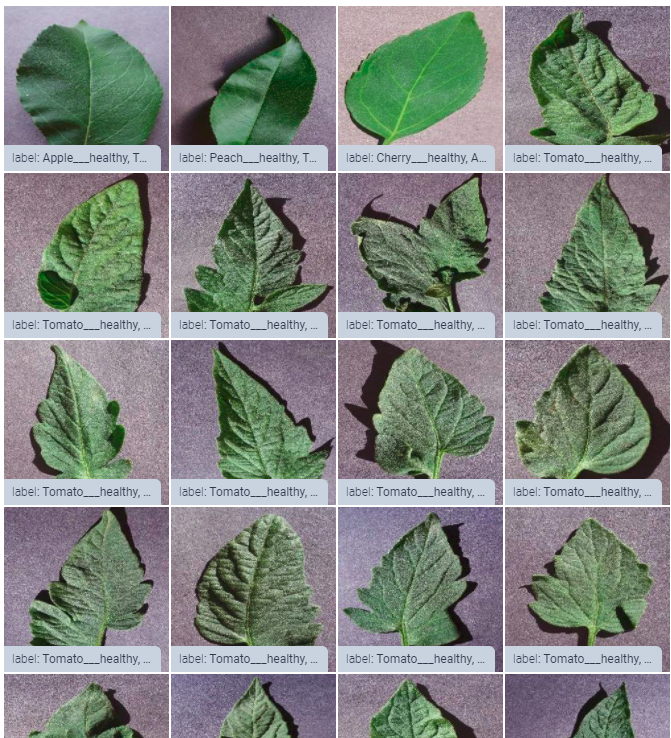
\includegraphics[width=0.8\linewidth]{images/plantvillage.png}
  \caption{\label{fig:samples}Exemplos de imagens de folhas no dataset PlantVillage (extraído de \url{https://paperswithcode.com/dataset/plantvillage}).}
\end{figure}

Contudo, infelizmente uma série de questões relacionadas à qualidade dos dados do \emph{PlantVillage} faz com que os ótimos resultados demonstrados nos trabalhos acadêmicos em questão não se traduzam para o contexto do cotidiano dos agricultores. Seja pela natureza das imagens, compostas de folhas de plantas em um plano de fundo de cor sólida e sem grandes variações na iluminação (o que não é reproduzido em fotos tiradas no campo) \citep{Yao2023, HughesS15, Singh:2017, Coletta2022Optimal} ou por problemas referentes a condições de captura (balanço de branco, exposição, foco) e padrões observados nos planos de fundo das imagens que se constituem como atributos que têm correlações espúrias com o rótulo das imagens e, por isso, acabam por facilitar muito a tarefa do modelo classificador desenvolvido \citep{Noyan:2022}.

Como comentado, a consequência desses vieses é que, apesar de artigos corriqueiramente publicados obterem resultados muito impressionantes na tarefa de classificação de doenças de plantas, esses resultados não se generalizam para situações reais e, portanto, nos dão uma falsa ideia de que o problema de classificação de doenças de plantas utilizando visão computacional já está resolvido. Isso acaba por ter o resultado oposto do esperado, atrasando o desenvolvimento tecnológico e científico.

Dessa forma, fica evidente que é necessário investir em alternativas para o desenvolvimento de conjunto de dados abertos, robustos e que tenham passado por curadoria. Somente assim avançaremos no desenvolvimento de modelos de visão computacional aplicados à detecção de doenças em plantas, com resultados que realmente farão a diferença no dia a dia dos agricultores que se beneficiariam dessas ferramentas abertas e acessíveis. Essa é a principal motivação desse trabalho de formatura supervisionado.

\section**{Objetivo}
O objetivo deste trabalho é desenvolver um sistema que possibilite a produção de melhores conjuntos de dados de visão computacional no domínio da agricultura. Para isso, a ideia proposta é a implementação de um sistema em que os usuários possam enviar fotos de, por exemplo, folhas de plantas doentes, para obter o diagnóstico da doença pelo sistema. As imagens enviadas pelos usuários serão acumuladas em um banco de dados de imagens e posteriormente revisadas por usuários especialistas, que poderão corrigir os diagnósticos feitos pelo sistema. Depois disso, as imagens revisadas passam a fazer parte de um novo conjunto de dados, que será incrementado com o tempo com as imagens enviadas para a plataforma. Dessa forma, consideramos que será possível produzir conjuntos de dados de boa qualidade e volume de maneira colaborativa.

\pagestyle{mainmatter}
\chapter{Descrição do problema e do sistema proposto}
Como comentado, o presente trabalho é motivado pela carência de conjuntos de dados abertos e robustos de imagens de doenças em folhas de plantas, que possibilitem o desenvolvimento de modelos de visão computacional com aplicabilidade prática no cotidiano dos produtores rurais.

\section{Considerações}
Para que um conjunto de dados com essa potencialidade seja desenvolvido, é preciso levar em conta algumas considerações importantes. Dentre elas, podemos destacar as seguintes:

\begin{enumerate}
{\bf \item  Volume considerável de dados:}

No contexto de \emph{deep learning}, modelos de visão computacional já se provaram muito efetivos. Contudo, é consenso que grandes quantidades de dados são necessárias para evitar \emph{overfitting}.

A ideia geral de sistemas supervisionados de \emph{machine learning}, é que, utilizando de algoritmos de otimização de uma função de perda --- que quantifica a performance do modelo atual --- os modelos em treinamento aprendam a reproduzir a função representada pelo conjunto de dados. Em que os dados de entrada são as variáveis independentes (no caso, imagens) e os rótulos são as variáveis dependentes \citep{Yaser:2012}. 

Nesse caso, quando não temos uma grande quantidade de dados, os modelos de aprendizado profundo (\emph{deeplearning}) têm a capacidade de aprender uma função que reproduz perfeitamente o conjunto de treinamento, é como se o modelo ``decorasse'' os dados ao invés de relacionar características importantes neles para chegar a respostas pertinentes \citep{Yaser:2012, Shorten2019A}. 

Por isso, esses sistemas necessitam de grandes quantidades de dados para funcionarem de maneira satisfatória \citep{Shorten2019A}. Então, para construir um conjunto de dados de qualidade para detecção de doenças em folhas de plantas, é importante que ele tenha um volume considerável.

{\bf \item Os dados devem contemplar a variabilidade dos casos de uso real da tecnologia:}
Para que modelos de \emph{machine learning} sejam capazes de generalizar bem, é necessário que, o conjunto de dados com os quais são treinados representem bem a diversidade dos dados que estarão presentes no cotidiano de uso da tecnologia resultante. Isso ocorre porque, quando os dados presentes nos casos de uso real da ferramenta forem muito diferentes dos dados de treinamento, o modelo simplesmente não terá tido contato com dados de tal natureza e, portanto performará pobremente. 

Um exemplo claro disso é o tipo de imagens presentes no \emph{dataset PlantVillage}. Essas imagens, com aspecto de ``laboratório'' (folhas retiradas das plantas e dispostas em superfícies planas e de cor sólida) certamente são diferentes das imagens disponíveis no contexto do campo: características como planos de fundo com alta variabilidade (plantas, paisagens, etc.) e folhas ainda presas nos galhos são exemplos disso.

{\bf \item Os dados devem passar por uma curadoria especializada:}

No domínio de detecção de doenças em plantas, uma avaliação de especialistas sobre os dados, para produzir rótulos corretos é de suma importância. Isso ocorre pois muitas vezes, não é fácil diferenciar as doenças entre si, devido à elevada similaridade entre sintomas e pelo simples fato dessa identificação não ser conhecimento ``comum''.

{\bf \item Não deve haver duplicatas ou ``quase-duplicatas'' nos dados:}

A presença de dados duplicados, ou ``quase-duplicados'' em conjuntos de dados é maléfica para o treinamento de modelos de \emph{machine learning}. Isso ocorre pois durante a etapa de treinamento, o modelo pode decorar padrões presentes nas imagens duplicadas e isso implica no comprometimento da performance dos modelos ao se deparar com dados inéditos \citep{Barz2019Do}. 

Além disso, a inclusão desses dados ``repetidos'' pode levar a uma similaridade elevada entre os conjuntos de treino e teste do \emph{dataset}. Nesse caso, como a avaliação do modelo é realizada com base no conjunto de teste, a presença de dados muito semelhantes pode artificialmente inflar as métricas de desempenho, resultando em uma avaliação irreal das capacidades do modelo e na pior capacidade de generalização no momento de implantação do modelo em campo \citep{Barz2019Do}.

\end{enumerate}


\section{Solução proposta}
Com o levantamento dessas considerações, formulamos uma abordagem de construção colaborativa de conjuntos de dados para detecção de doenças de plantas que se propõe a ser uma possível solução para a escassez de \emph{datasets} robustos, volumosos, confiáveis e abertos nesse domínio.

\subsection{Redução do escopo}
Para o desenvolvimento dessa solução, primeiramente reduzimos o escopo das tarefas propostas por grandes \emph{datasets} desse domínio \citep{Yao2023}. Tanto o \emph{PlantDoc} (um \emph{dataset} alternativo ao \emph{PlantVillage}, que oferece imagens sem a característica de imagens de ``laboratório'') quanto o próprio \emph{PlantVillage}, por exemplo, têm em suas classes o seguinte formato:
\begin{center}
    \texttt{(<espécie> : <condição>)}
\end{center}
Ou seja, além de identificar a doença que afeta a planta, o modelo também tem a tarefa de identificar a espécie da planta em questão. Na realidade, para o caso de uso abordado nesse trabalho (detecção de doenças em plantas) é esperado que o agricultor saiba, no mínimo, a espécie da planta que está cultivando. Desse modo, decidimos simplificar a tarefa para a {\bf detecção de doenças nas folhas de tomate}.

A escolha dessa cultura na redução do escopo do trabalho se deu pelo fato da hortaliça ser uma das mais consumidas no mundo e da tomaticultura ser de imensa importância no setor da agricultura brasileira, sendo uma das principais fontes de emprego e renda da produção agrícola e tendo um valor de produção bruto superior a 12,4 bilhões de reais em 2022, de acordo com dados do IBGE e matéria publicada no portal Revista Rural \footnote{\url{https://www.revistarural.com.br/2022/10/14/tecnologias-impulsionam-producao-nacional-do-tomate/}}.

\section{\emph{TomatoHealth}}
Desse modo, a ideia da solução proposta é implementar uma plataforma chamada \emph{TomatoHealth} que oferece a funcionalidade de detecção de doenças em folhas de tomate por meio de uma aplicação \emph{web}. Por meio dessa aplicação, os usuários podem submeter imagens das folhas de suas plantas e a aplicação retorna uma resposta sobre as doenças detectadas.

Para que isso ofereça uma possível solução para a escassez de conjuntos de dados robustos na tarefa de detecção de doenças em plantas, as imagens enviadas pelos usuários passam a fazer parte de um banco de dados. 

Então, a partir desse repositório de imagens enviadas pelos usuários, uma outra frente de atuação da plataforma permite que, para cada imagem armazenada no banco de dados, usuários privilegiados (especialistas do domínio) façam revisões da inferência efetuada pelo modelo de detecção de doenças. 

Depois dessa revisão, as imagens revisadas podem passar a integrar o conjunto de dados usado para a tarefa de detecção de doenças em folhas de tomate, fechando um ciclo de atualização contínua do conjunto de dados e melhorando, iterativamente, a robustez do conjunto de dados original.

É importante destacar que a solução implementada por essa primeira versão do \emph{TomatoHealth} aborda de maneira efetiva as seguintes considerações feitas sobre o problema tratado nesse trabalho de formatura supervisionado:

\begin{enumerate}
{\bf \item  Volume considerável de dados:} pois iterativamente, o volume do conjunto de dados é aumentado com imagens que passaram pelo crivo de especialistas;

{\bf \item Os dados contemplam a variabilidade dos casos de uso real da tecnologia:} pois as imagens que têm a possibilidade de passar a integrar o conjunto de dados são tiradas justamente do contexto de aplicação real da tecnologia;

{\bf \item Os dados passam por uma curadoria especializada:} pois a presença da figura dos especialistas atua na revisão e curadoria de todas as imagens que passam a fazer parte do conjunto de dados;

\end{enumerate}

Note que a consideração 

\begin{enumerate}
    \setcounter{enumi}{3}
    {\bf \item Não deve haver duplicatas ou ``quase-duplicatas'' nos dados}
\end{enumerate}

Não foi abordada por essa primeira versão de implementação do \emph{TomatoHealth}. Contudo, já planejamos a integração de algoritmos que façam busca por imagens semelhantes no conjunto de dados existente e as exiba para o especialista que está fazendo a revisão.

\begin{figure}
    \centering
    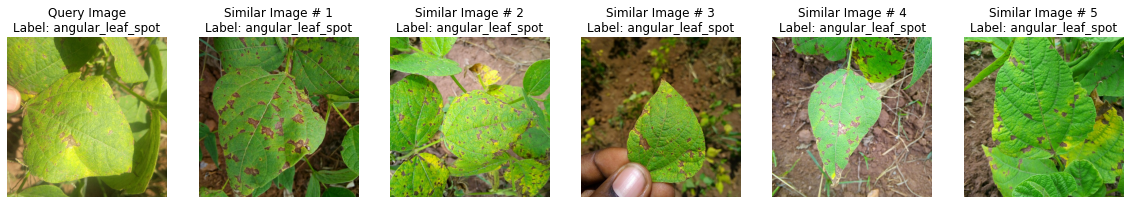
\includegraphics[width=1\linewidth]{images/results_one.png}
    \caption{\label{fig:similaridade}Exemplos de resultados do algoritmo de busca por imagens com base em similaridade. (extraído de \url{https://huggingface.co/blog/image-similarity}).}
\end{figure}

Caso a imagem que está sendo revisada apresente um grau de semelhança elevada com outras imagens que já fazem parte do conjunto de dados, o especialista terá a opção de descartar a amostra em questão. Essa funcionalidade, que fará com que a solução proposta contemple todas as considerações feitas no trabalho será melhor descrita na seção ~\ref{sec:próximos passos}.

\section{{Detalhes ``abstratos'' sobre o sistema} \label{sec:abst-det}}

Nessa seção, iremos descrever as capacidades esperadas do sistema desenvolvido sem detalhes de implementação.

\subsection{{\textit{Storyboard} do sistema}}

Uma ótima forma de começar o desenvolvimento de um sistema é demonstrar seus casos de uso e aplicações no mundo real por meio de um \textit{Storyboard}. Uma técnica muito empregada por estúdios de animação, pois produzir desenhos para cada quadro de uma animação é uma tarefa demorada, e desenhar um quadro que não será usado é um desperdício (similar ao desenvolvimento de código). Além de ser rápido de esboçar, o \textit{Storyboard} permite demonstrar informações sobre um sistema que seria dificilmente explicado por texto, e também transmite informações essenciais de um sistema: usuários, contexto, sequência de tarefas de seu sistema e como seu sistema traz satisfação \citep{klemmer2016}. Sendo assim, a Figura \ref{fig:storyboard} demonstra o \textit{Storyboard} feito para o \emph{TomatoHealth}.

Na Figura \ref{fig:storyboard}, enumeramos as ações dos quadrinhos:

\begin{enumerate}
    \item Um tomateiro doente
    \item Um fazendeiro encontra seu tomateiro doente
    \item Ele tira uma foto da sua folha
    \item Ele fica alegre em descobrir a doença e como cuidar de seu tomateiro, com a ajuda de uma Inteligência Artificial
    \item A imagem tirada pelo fazendeiro é salva num banco de dados abertos
    \item Um especialista analisa as imagens salvas
    \item As imagens analisadas por um especialista são usadas para treinar a Inteligência Artificial
\end{enumerate}

\begin{figure}[ht]
    \centering
    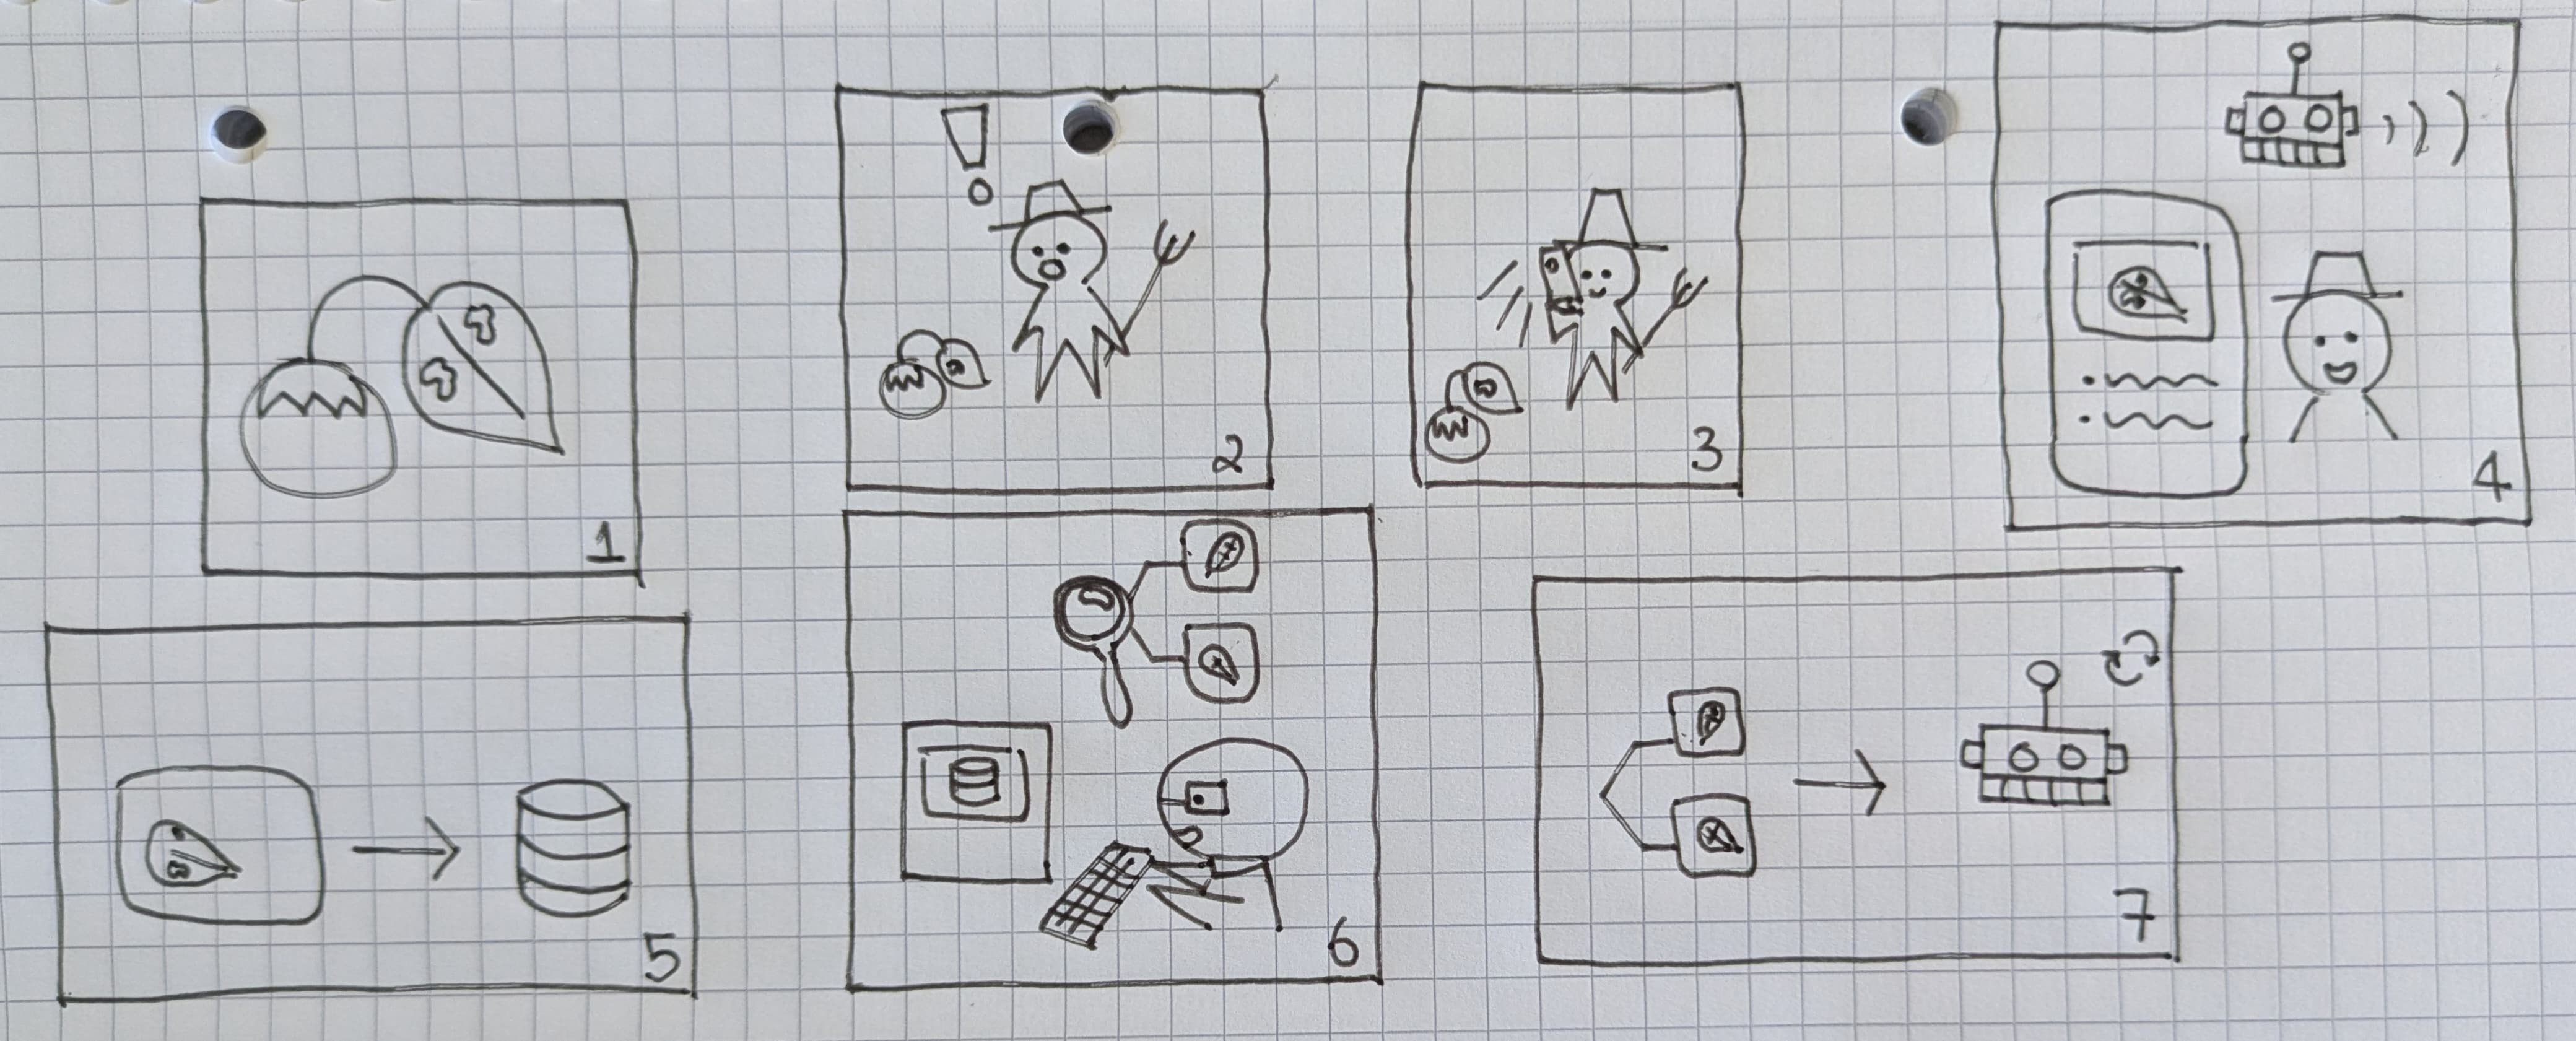
\includegraphics[width=\textwidth]{images/storyboard.jpg}
    \caption{Storyboard do desenvolvimento do sistema}
    \label{fig:storyboard}
\end{figure}

\subsection{{Descrição geral sobre o sistema}}

Já tendo uma breve noção sobre a atuação do \emph{TomatoHealth} por nosso \textit{Storyboard}, também é importante descrever o sistema de maneira geral, para comentar sua pertinência aos assuntos tratados nesse trabalho, e destacar como ele se relaciona ao problema.

As próximas seções separam os componentes do sistema do \emph{TomatoHealth}, para que a Seção \ref{sec:implementacao_sistema} os detalhe de maneira técnica.

\subsubsection{{Interface do Usuário Geral} \label{sec:abst-geral}}

Nossa interface \textit{web} deve permitir ao usuário geral:

\begin{itemize}
    \item entender o papel da ferramenta
    \item tirar ou escolher uma foto de folha de tomate
    \item enviar essa foto para análise
    \item receber um \textit{feedback} sobre a saúde de seu tomateiro
\end{itemize}

Uma parte importante dessa interface é estimular o usuário a tirar uma foto de sua folha a partir de seu celular, para que essas imagens quando armazenadas e classificadas sirvam de dados em casos de usos reais em nosso \textit{dataset}.

Com esse objetivo em mente, priorizamos o desenvolvimento \textit{mobile-first}, e permitimos o usuário a acessar a câmera de seu celular, assim como o instruímos de como tirar uma foto adequada, tanto para um \textit{feedback} quanto um dado melhor em nosso \textit{dataset}.

\subsubsection{{Interface do Usuário Especialista} \label{sec:abst-esp}}

Na interface do usuário especialista, ele deve ser capaz de:

\begin{itemize}
    \item autenticar com seu e-mail e sua senha
    \item ver as imagens tiradas por usuários comuns
    \item demarcar na imagem as diferentes classes que uma folha de tomate pode ter
\end{itemize}

Com isso, as imagens ficam com suas classes demarcadas por um quadrado, e inseridas em nosso banco de dados, para retreinamento do nosso modelo. 

\subsubsection{{\emph{Back-end}}\label{sec:back-end-intro}}

Nosso \emph{back-end} deve comportar:

\begin{itemize}
    \item a criação de usuários especialistas
    \item um banco de dados com as imagens enviadas por usuários comuns e as imagens a serem usadas no modelo de detecção
    \item o treinamento do modelo
    \item um servidor que recebe uma imagem, realiza a detecção, e faz uma chamada para uma \emph{LLM} recomendar cuidados a serem feitos com o tomateiro de acordo com as classes detectadas
    \item a inserção de imagens enviadas por usuários comuns e de imagens anotadas por especialistas no banco de dados
\end{itemize}

Dessa forma, o sistema faz o treinamento do modelo de maneira periódica com dados revisados por especialistas, e retorna um \textit{feedback} com as detecções do modelo a um usuário comum.

\section{{Sistemas similares -- detecção de doenças e sistemas colaborativos}}

Ao pesquisar por \textit{"plant diagnosis"} na \textit{Google Play} \footnote{\url{https://play.google.com/store/apps/}}, encontramos dezenas de aplicativos capazes de identificar culturas e/ou doenças por meio de fotos. Um dos mais populares, com mais de $10$ milhões de downloads, é o \textit{Plantix} \footnote{\url{https://plantix.net/pt/}}.

Ademais, na pesquisa por sistemas no âmbito de ciência colaborativa, encontramos duas referências semelhantes quanto a nossa proposta de sistema por compartilharem fotos fornecidas por usuários para a utilização em pesquisa, são elas: \textit{iNaturalist} \footnote{\url{https://www.inaturalist.org/}} e \textit{Zooniverse} \footnote{\url{https://www.zooniverse.org/}}.

\subsection{\textit{Plantix}}

Segundo sua página, o aplicativo tem o mesmo propósito de nosso \textit{TomatoHealth}, mas para diversas culturas. Entretanto, além do sistema identificar doenças e propor tratamentos, ele fornece ao usuário o contato com especialistas para sanar dúvidas, e também conta com uma biblioteca sobre doenças em plantas.

\subsection{\emph{iNaturalist}}

O \textit{iNaturalist} é uma comunidade onde usuários observam organismos vivos com suas câmeras, obtêm detalhes, e compartilham suas fotos com outros entusiastas. A plataforma também faz com que as fotos sejam compartilhadas com repositórios de dados abertos como o \textit{Global Biodiversity Information Facility} (GBIF), e conecta usuários comuns com especialistas, capazes de identificar diferentes espécies.

\subsection{\emph{Zooniverse}}

Já o \textit{Zooniverse} é constituído por projetos em diferentes áreas da ciência: Artes, Biologia, Clima, História, etc., em quais voluntários classificam dados disponibilizados por um projeto e se conectam com especialistas. O propósito da ferramenta é descrito como "pesquisa com base em pessoas", de forma a destacar o papel do voluntário na análise dos dados e no fomento de pesquisas. No dia de hoje (2 de novembro de 2024), o site conta com 2.783.522 voluntários e 846.112.376 classificações.

\chapter{Aplicação de \emph{Machine Learning} no projeto}
No projeto \emph{TomatoHealth}, que possui a funcionalidade de detecção de doenças em imagens de folhas de tomate, as técnicas de \emph{Machine Learning} desempenham um papel fundamental. No campo da visão computacional aplicada à agricultura, é comum o uso de modelos de Inteligência Artificial para tarefas como classificação de imagens ou detecção de objetos.

Esses métodos tornam-se indispensáveis em situações onde a complexidade do problema torna impraticável ou mesmo impossível desenvolver um programa de computador tradicional baseado em regras fixas capaz de oferecer uma boa solução. Como por exemplo, determinar a doença presente em uma folha a partir de sua imagem. Em casos como esse, recorremos a técnicas de aprendizado de máquina, que oferecem a capacidade de aprender padrões complexos a partir de dados.

No contexto de aprendizado de máquina supervisionado, é necessário dispor de um conjunto de dados rotulados. Esses dados são usados para treinar o modelo de IA, permitindo que ele aprenda a identificar os padrões que caracterizam cada rótulo. Uma vez treinado, o modelo é capaz de generalizar esse conhecimento para realizar predições precisas em novos dados de entrada, predizendo seus rótulos.

\section{Classificação vs Detecção}
Para que o processo de treinamento do modelo de visão computacional seja possível, primeiro é necessário escolher a arquitetura de rede neural que será utilizada. Contudo, ainda antes disso, é necessário definir qual é a tarefa que devemos realizar e um \emph{dataset} já existente para efetuar o treinamento desse primeiro modelo que será integrado à plataforma.

Até agora, a expressão: ``detecção de doenças em imagens de folhas de plantas''; que resume qual é o objetivo do modelo de visão computacional incorporado ao \emph{TomatoHealth} ainda não foi muito bem definida.

É importante esclarecer isso pois, nesse domínio, não há um consenso entre os \emph{datasets} publicamente disponíveis. Isso ocorre pois a tarefa proposta pelo \emph{dataset PlantVillage}, e, portanto, a tarefa mais popular nesse domínio, é a de {\bf classificação}. Isto é, o modelo treinado recebe uma imagem como entrada e então classifica essa imagem como tendo um dentre os diversos rótulos possíveis.

Já o \emph{dataset PlantDoc}, propõe uma tarefa de {\bf detecção de objetos}. Como já comentado, esse \emph{dataset} surgiu para ser uma alternativa ao \emph{PlantVillage}. Podemos comentar sobre a mudança das caracteríticas das imagens, que no \emph{PlantDoc} são oriundas do campo e não obtidas em um ``ambiente controlado'', mas uma das melhorias conceituais mais importantes que foi proposta é justamente a mudança da tarefa de classificação para a de detecção de objetos.

Ao pensar no domínio da agricultura e nos casos de uso dessa tecnologia de visão computacional para identificar doenças em folhas de plantas, não é difícil perceber que a tarefa de detecção de objetos é a mais adequada. 

Para que a tarefa de classificação de imagens seja coerente nesse contexto, é necessário que somente uma folha esteja presente na imagem. Para isso, um agricultor no campo teria de retirar a folha da planta, colocá-la sobre uma supefície plana e então efetuar a captura da imagem.

Já no caso da tarefa de detecção de objetos, bastaria identificar a planta de interesse e efetuar a captura da imagem de modo que as folhas afetadas pela doença estejam presentes na imagem.

Ao compararmos essas duas abordagens diferentes, a etapa adicional inerente à tarefa de classificação (de ser necessário retirar uma folha da planta e só então efetuar a captura da imagem) só seria justificada se isso significasse em uma performance muito superior dos modelos de visão computacional baseadas no conceito de classificação, o que não é o caso \citep{Singh2020}.

Desse modo, é mais interessante trabalharmos com a tarefa de detecção, em que, dado uma imagem de planta com diversas folhas, as folhas presentes na imagem serão detectadas e então classificadas de acordo com as diversas doenças possíveis.

Considerando o fato do \emph{PlantDoc} ter sido construído após a constatação de que haviam problemas profundos com o \emph{PlantVillage} e ter proposto essas melhorias para tentar se consolidar como um novo padrão de \emph{dataset} público para essa tarefa, decidimos escolhê-lo para ser o \emph{dataset} de base para o modelo de visão computacional do \emph{TomatoHealth}.

Para performar essa tarefa de detecção de objetos, escolhemos a família de modelos \emph{YOLO}, que explicaremos em detalhes na seção \ref{sec:modelo}

\section{Entendendo detecção de objetos em \emph{Machine Learning}}
A detecção de objetos tem o objetivo de resolver uma das questões fundamentais de aplicações de visão computacional. Identificar o que são os objetos e onde eles estão localizados nas imagens. Isso é feito por meio da detecção de instâncias de objetos pertencentes à classes específicas nas imagens em questão, com o uso de \emph{bounding boxes} --- retângulos que envolvem os objetos detectados e indicam sua classe \citep{Zou2019Object}.

\begin{figure}[htb!]
    \centering
    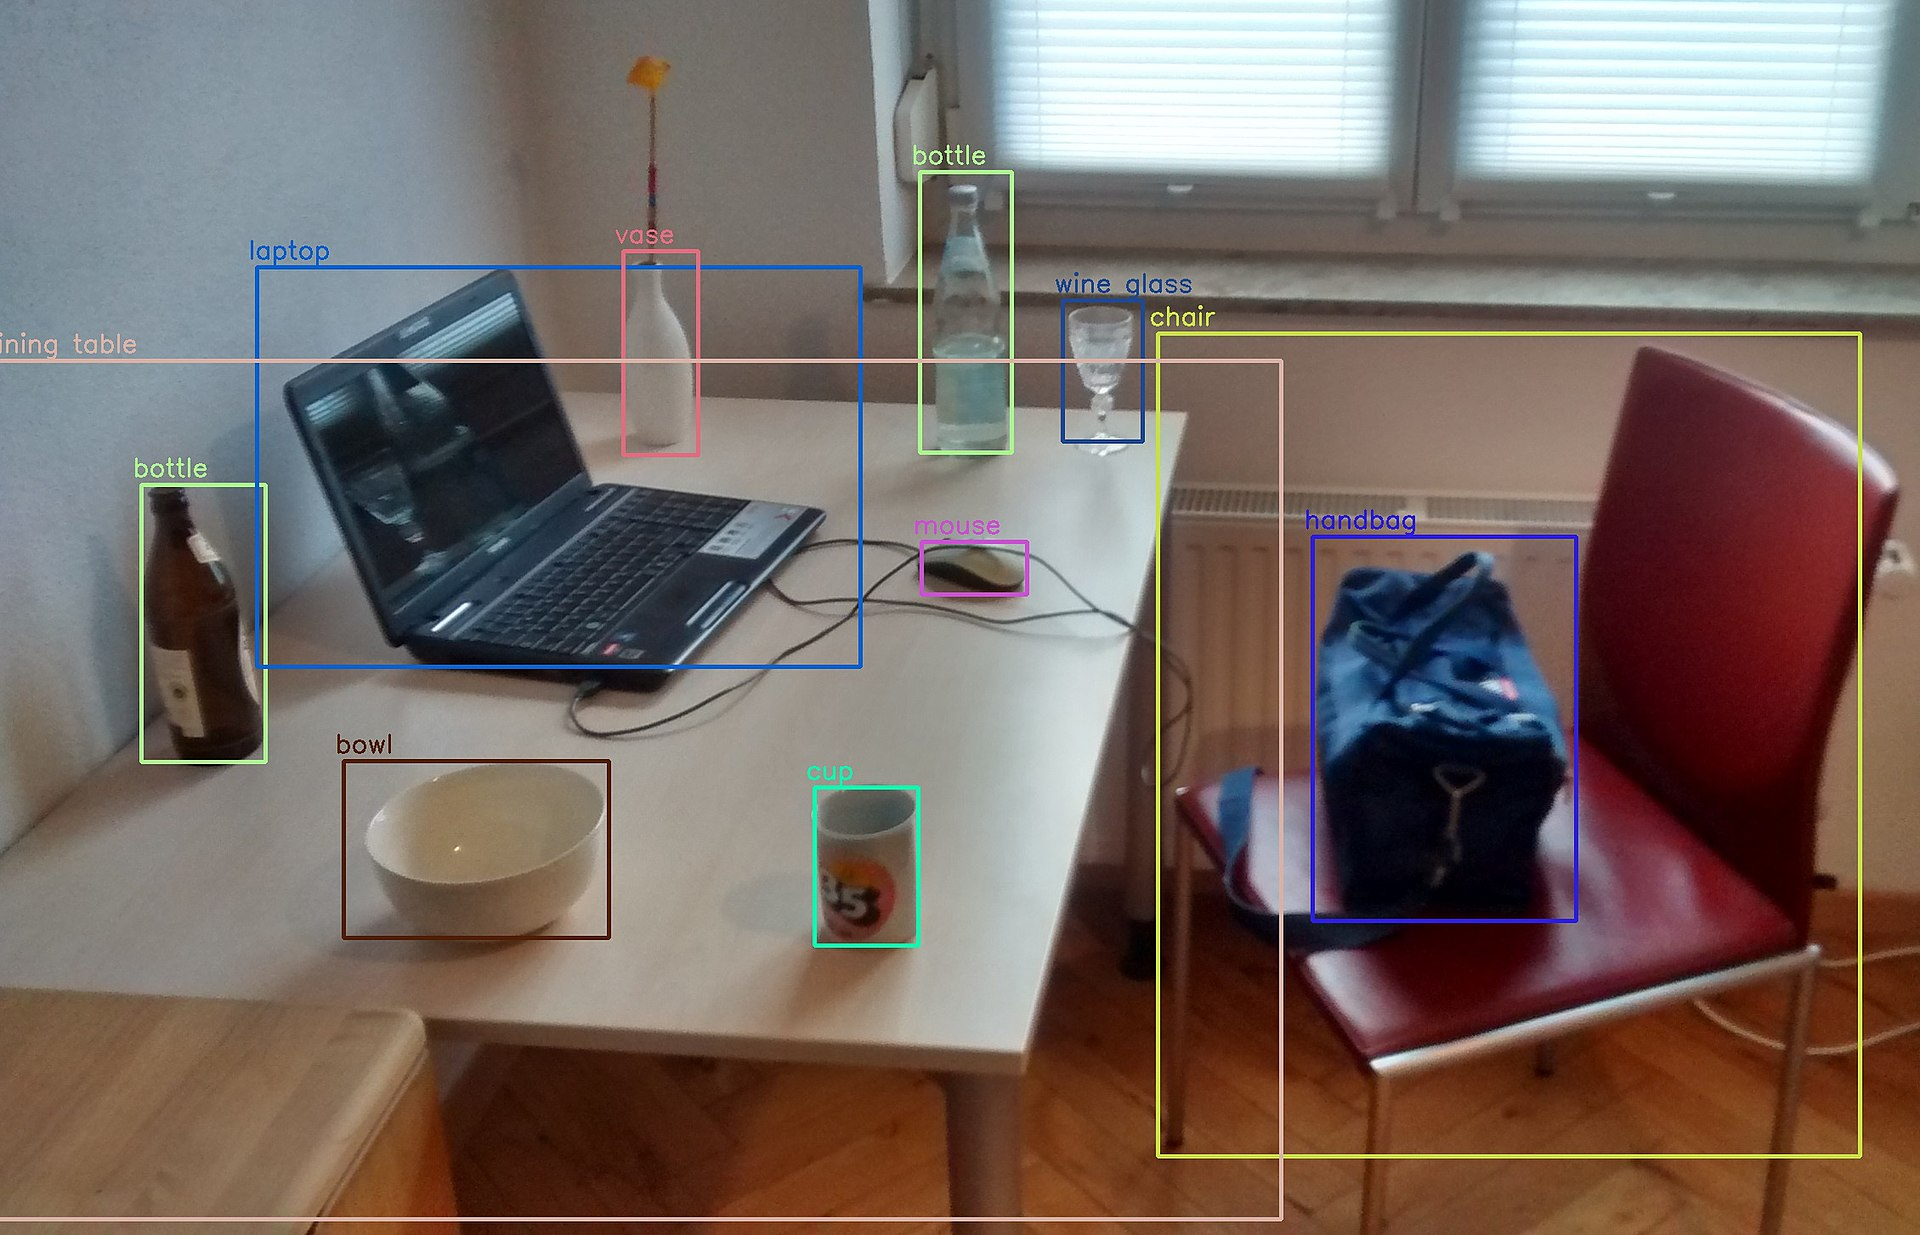
\includegraphics[width=0.8\linewidth]{images/bounding_boxes.png}
    \caption{\label{fig:bounding_boxes} Exemplo de detecção de objetos em uma imagem utilizando \emph{bounding boxes}. Imagem extraída de \citeauthor{MTheiler}, trabalho próprio, licenciada sob CC BY-SA 4.0. Disponível em: \url{https://commons.wikimedia.org/w/index.php?curid=75843378}.}
\end{figure}

A tarefa de detectar objetos em imagens não é nova, e por ter muitas aplicações como detecção de faces e corpos humanos e servir como base para outras tarefas como direção autônoma, \emph{image captioning} --- que corresponde à tarefa de descrever imagens com textos de linguagem natural ---, aplicações em sistemas com câmeras de segurança, etc. Há uma evolução rápida nesse campo da ciência desde os anos 1990 \citep{Zou2019Object, Zhao2018Object}. Podemos observar essa evolução ao considerarmos o crescimento exponencial no número de publicações que vêm ocorrendo nessa área de conhecimento:
\begin{figure}[htb!]
    \centering
    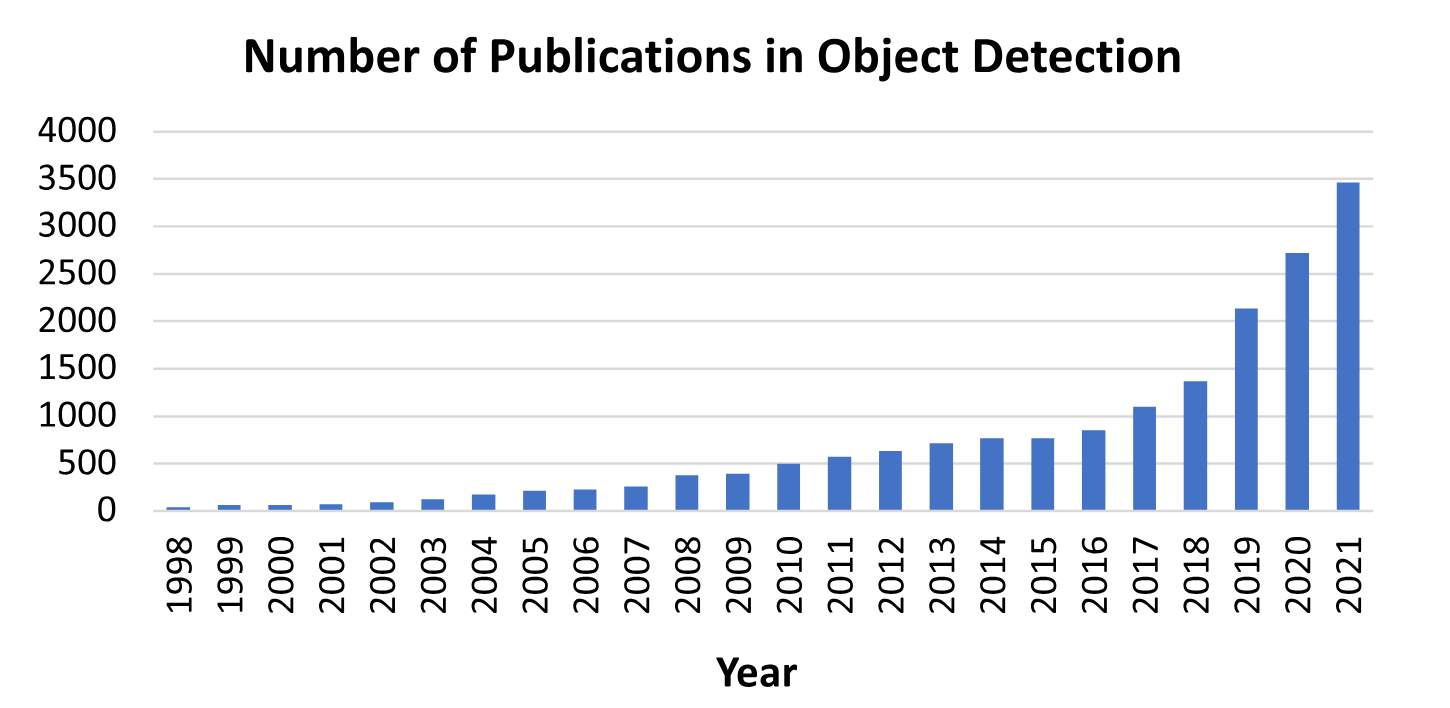
\includegraphics[width=0.8\linewidth]{images/obj_detection_evo.png}
    \caption{\label{fig:obj_evo}Crescimento do número de publicações relacionadas à detecção de objetos ao longo dos anos. (extraído de \citep{Zou2019Object}).}
\end{figure}

O motivo da aceleração significativa na produção de conhecimento científico nessa área do conhecimento foi uma mudança de paradigma considerável: a introdução de técnicas de \emph{deep learning} nessa tarefa de visão computacional. Dessa forma, podemos afirmar que a história da detecção de objetos pode ser compreendida a partir de dois períodos históricos que iremos abordar a seguir: detecção de objetos com uma abordagem tradicional (anterior a 2014) e detecção de objetos baseada em \emph{deep learning} (depois de 2014) \citep{Zou2019Object}.

\subsection{Detecção de objetos com uma abordagem tradicional}
Antes do advento das técnicas de \emph{deep learning}, os métodos para detecção de objetos em imagens dependiam da extração manual de representações (características) eficazes para a inferência esperada. Os algoritmos mais eminentes dessa época utilizavam janelas deslizantes na imagem com filtros compostos pelas características extraídas manualmente. 

Por exemplo, no algorítimo de Viola-Jones, a imagem é percorrida por janelas deslizantes de diversas escalas contendo características presentes em rostos humanos (Haar \emph{features}). Dessa forma, a depender da correspondência das características com a imagem, uma face poderia ser acusada como detectada ou não naquela localidade, isso é feito com classificadores em cascata \citep{Viola}.

Por outro lado, o método \emph{HOG (Histogram of Oriented Gradients)} é um método em que as caraterísticas da imagem são obtidas por meio da computação de gradientes em pequenas porções da imagem. Para cada pequena localidade, o histograma resultante era concatenado aos demais, formando um mapa de características representativo de bordas e texturas. Com a aplicação desse mapa de características em classificadores como \emph{SVMs} (\emph{Support Vector Machines} \citep{Cortes1995Support-Vector}), é possível detectar objetos e essa combinação foi inicialmente implementada para detecção de faces \citep{HOG}.

De maneira geral, perceba que podemos resumir as abordagens tradicionais de detecção de objetos como a extração manual de características das imagens (Haar \emph{features} ou mapas de gradientes oriundos de \emph{HOG}) e então essas características passavam por classificadores simples \citep{Viola, HOG}.

Contudo, essas abordagens eram limitadas e os novos métodos com \emph{deep learning} superaram os desempenhos desses algoritmos mais tradicionais \citep{Zou2019Object}.

\subsection{Detecção de objetos baseada em \emph{deep learning}}
Depois de um tempo, a performance de detectores de objetos com representações extraídas manualmente chegou a ficar saturada. Então, com o advento das técnicas de \emph{deep learning}, especialmente das redes neurais convolucionais (\emph{CNNs}), passou a ser possível processar imagens em seu formato bruto e obter automaticamente representações de alto nível de suas características. Isso impulsionou um avanço significativo na precisão e eficiência dos métodos de detecção de objetos, marcando um salto evolutivo nessa tarefa de visão computacional \citep{Zou2019Object}.

\subsubsection{Fundamentos de redes neurais convolucionais}
Redes neurais podem ser entendidas como funções não lineares extremamente complexas. Esse artifício matemático é constituído por nós --- neurônios --- organizados em camadas. Cada nó efetua uma combinação linear dos valores oriundos dos nós da camada anterior e então passa o resultado dessa operação por uma função não linear --- função de ativação. 

Podemos pensar que a relação entre os dados de entrada de um \emph{dataset} e cada um dos seus rótulos é regida por uma função. Por meio do método do gradiente descendente e da técnica de \emph{backpropagation}, conseguimos fazer com que os parâmetros da rede neural (pesos das combinações lineares) se adaptem de modo a reproduzir essa função.

As redes neurais convolucionais são uma evolução das redes neurais convencionais. Elas são especialmente boas lidando com imagens. São constituídas por três tipos de camadas diferentes:

\paragraph{Camadas convolucionais} aplicam a operação de convolução nos dados que chegam à essa camada. Nesse caso, os pesos do \emph{kernel} da convolução são aprendidos como parâmetros da rede neural.

\paragraph{Camadas de \emph{pooling}} são camadas utilizadas para redimensionar os dados de entrada. Tanto aqui quanto em relação às camadas convolucionais, podemos pensar que os dados de entrada são imagens. Geralmente, as camadas de \emph{pooling} não apresentam parâmetros aprendíveis pela rede (treináveis). A técnica mais utilizada é a denominada \emph{max-pooling}, em que a camada visa preservar o sinal privilegiado pela camada convolucional anterior.

\paragraph{Camadas \emph{fully connected}} são camadas semelhantes às presentes nas redes neurais originais. Geralmente são utilizadas para relacionar --- de maneira treinável --- os resultados das camadas abordadas anteriormente. Constituem camadas que utilizam as características extraídas pelas camadas convolucionais e de \emph{pooling}, para efetuar a classificação. Isso, no caso de um problema de classificação, evidentemente.

\subsubsection{Principais modelos para detecção de objetos com \emph{deep learning}}
Com o avanço do \emph{deep learing} e das redes convolucionais, esses novos conceitos foram introduzidos ao contexto de detecção de objetos com a introdução de \emph{Regions with CNN features} (\emph{RCNNs}) \citep{Zou2019Object, rcnn1, rcnn2}.

A ideia por trás do conceito de \emph{RCNN} é bem direta. Primeiro um conjunto de regiões na imagem é obtido por meio de algoritmos de busca. Depois disso, as representações de cada região é obtida ao passá-las (adaptadas para um tamanho fixo) por uma rede convolucional. Por fim, classificadores como \emph{SVMs} \citep{Zou2019Object}.

Ao longo do tempo, esforços foram sendo feitos para aumentar a velocidade da detecção de objetos com \emph{CNNs}. A abordagem de \cite{SPPNet} utiliza o conceito de \emph{spatial pyramidal pooling}, com esse conceito, as regiões de interesse (\emph{RoI}) são obtidas diretamente no mapa de \emph{features}, o que aumenta muito a velocidade de todo o processo.

O \emph{spatial pyramidal pooling} funciona ao subdividir a \emph{RoI} em ``grades de células'' e aplicar a operação de \emph{max pooling} em cada célula. Desse modo, ao final do \emph{spatial pyramidal pooling}, teremos um vetor de representações de tamanho fixo, independente do tamanho da \emph{RoI} \citep{SPPNet}. Depois disso, esses vetores passam por algoritmos de classificação como \emph{Support Vector Machines (SVMs)}. A possibilidade de uso desse vetor de tamanho fixo foi uma das principais contribuições da \emph{SPPNet} \citep{Zou2019Object}.

Depois disso, \cite{fastRCNN} introduziu a \emph{Fast R-CNN}, que possibilitou o treinamento de uma única rede neural capaz de realizar simultaneamente a regressão das \emph{bounding boxes} (isto é, um ajuste fino das \emph{RoIs} inicialmente propostas por algoritmos de busca) e das classificações. Isso representou um avanço em relação à \emph{SPPnet}, que processava a obtenção das \emph{RoIs} e a classificação das regiões de interesse em etapas distintas, o que tornava o processo mais lento e menos eficiente.

É notável que, a princípio, os métodos de detecção baseados em \emph{CNNs} eram baseados em duas etapas: a proposta das regiões de interesse e, depois, a classificação dessas regiões. A partir de 2015, a tarefa de detecção de objetos com \emph{CNNs} passou a ser feita em somente uma etapa. 

A arquitetura \emph{YOLO (You Only Look Once)} é uma grande representante dessa nova abordagem, permitindo obter as coordenadas das \emph{bounding boxes} e suas classificações em uma única passagem pela rede neural, viabilizando a detecção de objetos em tempo real. Pioneira na detecção de objetos em uma etapa, a arquitetura \emph{YOLO} ganhou popularidade por seus bons resultados em acurácia e velocidade \citep{Zou2019Object}, sendo, por isso, a escolhida para a tarefa de detecção de objetos no \emph{TomatoHealth}.

\section{\emph{YOLO} (\emph{You Only Look Once}) \label{sec:yolo}}
\label{sec:modelo}
\subsection{Contextualização}
A arquitetura de rede neural para detecção de objetos \emph{YOLO} foi introduzida em 2016 com o trabalho de \cite{yolo}. Desde então, diversas evoluções e melhorias foram incorporadas ao modelo. Ao longo dos anos, novas versões dessa arquitetura foram lançadas, indo do \emph{YOLOv1} ao \emph{YOLOv8} em 2023 e até mesmo modelos mais atuais como o \emph{YOLO11}, lançado em 2024 \citep{yolo, yolov8_2023, yolo11_2024}. Por haver mais informação disponível sobre o modelo \emph{YOLOv8} e pelo fato de ainda ser um modelo novo e com performances muito satisfatórias, essa foi a arquitetura escolhida para o projeto. Além disso, apesar dessa evolução entre versões, os conceitos fundamentais e as ideias por trás do \emph{YOLO} ainda podem ser utilizadas para entender seu funcionamento.


Na aplicação \emph{TomatoHealth}, utilizamos o modelo \emph{YOLOv8}. No entanto, o propósito deste texto não é aprofundar em detalhes específicos ou otimizações exclusivas desta versão, mas sim oferecer uma visão geral de como o \emph{framework YOLO} funciona. A seguir, apresentaremos os conceitos primeiro introduzidos em 2016 com o \emph{YOLOv1} e então discutiremos os avanços e melhorias que foram incorporados à arquitetura do \emph{YOLOv8}.

\subsection{Conceitos fundamentais do \emph{YOLO}}
Como já comentado, a principal ideia proposta pela arquitetura \emph{YOLO} é efetuar a detecção de objetos em uma só etapa. Dessa maneira, uma única rede neural faz a predição das \emph{bounding boxes} e das classificações. Com somente um \emph{forward pass}.

\paragraph{Passo a passo do \emph{YOLOv1}:}
No \emph{YOLOv1}, isso é feito por meio do artifício de enxergar o problema de detecção de objetos como puramente um problema de regressão. Isso significa que o problema é formulado de tal modo que os valores preditos pelo modelo são contínuos. Mesmo que a classificação esteja envolvida na tarefa de detecção de objetos, o \emph{YOLOv1} não trabalha com a predição de valores discretos para as classes.

O funcionamento da arquitetura \emph{YOLO} segue o seguinte passo a passo:

\begin{itemize}
    \item Escolhemos uma imagem como \emph{input} para o modelo;
    \item A redimensionamos para um tamanho fixo --- no artigo original, $448 \times 448$;
    \item Dividimos a imagem em $S \times S$ quadrados (\emph{grid cells}) --- no artigo original, $S = 7$;
\end{itemize}

É importante evidenciar que, nesse contexto, cada \emph{grid cell} terá a capacidade de prever um objeto cujo centro esteja localizado no seu interior.

\begin{figure}
    \centering
    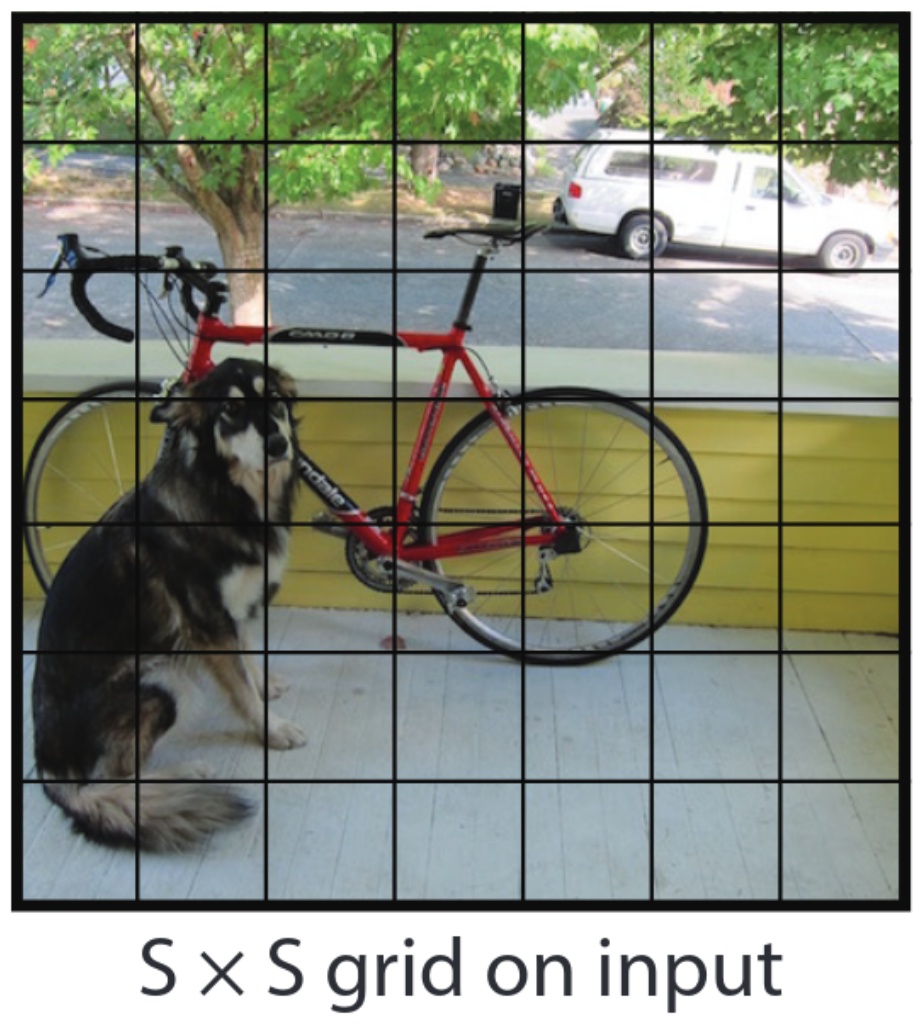
\includegraphics[width=0.5\linewidth]{images/grid_cells.png}
    \caption{\label{fig:grid_cells} Figura que ilustra a as \emph{grid cells} do \emph{YOLOv1} em uma imagem. Imagem extraída de \cite{yolo}.}
\end{figure}

Para treinar o modelo \emph{YOLOv1}, considere o seguinte rótulo de \emph{bounding box}:$(x, y, w, h)$; onde $(x,y)$ corresponde ao centro da \emph{bounding box} e $w$ e $h$ à sua largura e altura, respectivamente. Perceba que no rótulo, os valores de $x, y, w$ e $h$ são valores absolutos relativos aos \emph{pixels} da imagem inteira. Contudo, a previsão do modelo e, portanto, os valores alvo são relativos à \emph{grid cell} em que o centro da \emph{bounding box} está localizado. Dessa forma, uma importante etapa de pre-processamento dos dados que passam pela arquitetura do \emph{YOLOv1} é a normalização desses valores para que sejam relativos à \emph{grid cell}. Isso é feito da seguinte maneira:

Os componentes de uma \emph{bounding box} predita são: $(\Delta{x}, \Delta{y}, \Delta{w}, \Delta{h})$; onde:

\begin{align}
\Delta{x} = \left(x - x_a \right) / \left( L / S\right)\\
\Delta{y} = \left(y - y_a \right) / \left( L / S\right)
\end{align}

Perceba que $\left( L / S\right)$ é justamente o tamanho do lado de uma \emph{grid cell}, pois $L$ é o comprimento do lado da imagem. Além disso, $(x_a, y_a)$ corresponde às coordenadas do canto esquerdo superior da \emph{grid cell}. Desse modo, note que $\Delta{x}$ e $\Delta{y}$ correspondem ao centro da \emph{bounding box} em uma posição relativa à \emph{grid cell} em que ele se encontra.

De maneira análoga:

\begin{align}
\Delta{x} = \left(x - x_a \right) / \left( L / S\right)\\
\Delta{y} = \left(y - y_a \right) / \left( L / S\right)
\end{align}

Então, $\Delta{w}$ e $\Delta{h}$ correspondem ao tamanho da \emph{bounding box} em relação às medidas de uma \emph{grid cell}.

Além desse processamento, outra coisa que deve ser feita é a codificação dos rótulos da classe de cada objeto. Esse processo é chamado \emph{One-hot encoding} e nele, a classe de um objeto é definida por um vetor de tamanho $N$ em que $N$ é a quantidade de classes que o problema possui e é tal que:
\begin{equation}
y_i = 
\begin{cases} 
1, & \text{se } i = k \\
0, & \text{se } i \neq k 
\end{cases}
\end{equation}
onde $i$ representa o índice da classe atual, e $k$ é o índice da classe alvo para o objeto em questão. Ou seja, o vetor resultante do \emph{one-hot encoding} possui valor 1 apenas na posição da classe do objeto e 0 nas demais posições.

Sobre os conceitos envolvidos com as \emph{grid cells} do \emph{YOLOv1}, resta explicar que, cada \emph{grid cell} terá um número $B$ de \emph{bounding boxes} candidatas à englobarem o objeto cujo centro está dentro de seus limites. No artigo original, $B = 2$. Assim, a \emph{bounding box} que tiver o maior valor de confiança de que contém um objeto será a escolhida como \emph{bounding box} para essa \emph{grid cell}.

Para continuar o entendimento dos passos envolvidos na detecção de objetos do \emph{YOLOv1}, precisamos saber como é o resultado da tarefa de detecção de objetos sobre uma imagem. Desse modo, após o \emph{forward pass}, temos o seguinte vetor de predição:

$$
\left[
\Delta\hat{x}_1, \, \Delta\hat{y}_1, \, \Delta \hat{w}_1, \, \Delta\hat{h}_1, \, \hat{c}_1, \, \Delta\hat{x}_2, \, \Delta\hat{y}_2, \, \Delta\hat{w}_2, \, \Delta \hat{h}_2, \, \hat{c}_2, \, \hat{p}_1, \, \hat{p}_2, \, \dots, \, \hat{p}_{20} 
\right]
$$

onde:
$$
\left[
\Delta\hat{x}_i, \, \Delta\hat{y}_i, \, \Delta \hat{w}_i, \, \Delta\hat{h}_i, \, \hat{c}_i
\right]^B_{i=1}
$$

Corresponde às coordenadas das \emph{bounding boxes} preditas pela \emph{grid cell} em questão e $\hat{c}$ a confiança de que, nessa \emph{grid cell} o centro de um objeto esteja localizado.

Além disso, 

$$
\left[
\hat{p}_1, \, \hat{p}_2, \, \dots, \, \hat{p}_{20} 
\right]
$$

São os valores das probabilidades preditas para cada classe, no modelo proposto por \emph{One-hot encoding}. Temos o número de 20 classes pois o \emph{YOLOv1} foi concebido para atuar com o \emph{dataset} PASCAL VOC \citep{yolo}.

Assim, para cada \emph{grid} cell, temos um vetor de tamanho $1 \times 30$ de resultado. Como são $7 \times 7$ \emph{grid cells} em uma imagem, temos de resultado de um \emph{forward pass} um vetor de tamanho $7 \times 7 \times 30$.

Nesse ponto, perceba que, para obtermos as coordenadas e as dimensões das \emph{bounding boxes}, precisamos passar pelo seguinte processo (estamos revertendo a normalização feita no inicio do \emph{forwar pass}):

$$
\begin{cases}
x_1 = \Delta x_1 \times \left(L / S \right) + x_a \\
y_1 = \Delta y_1 \times \left(L / S \right) + y_a \\
w_1 = \Delta w_1 \times L \\
h_1 = \Delta h_1 \times L
\end{cases}
$$

E, para obter as informações sobre a classe, temos:

\begin{itemize}
    \item \textbf{Classe do objeto}: A classe \( l \) do objeto é dada por:
   $$
   l = \arg\max(p_1, p_2, \dots, p_{20})
   $$

    \item \textbf{Confiança da classe}: A confiança da classe (\( \hat{c}_1 \) ou \( \hat{c}_2 \)) é calculada multiplicando a confiança da \emph{bounding box} pelo valor máximo de probabilidade \( p \) entre as classes. Dessa forma:
       $$
       p = \max(p_1, p_2, \dots, p_{20})
       $$
       e
       $$
       \hat{c} = c_i \times p
       $$
       onde $c_i = \max\{c_1, c_2\}$.
\end{itemize}
Então, ao exibir as informações sobre o objeto detectado, levamos em consideração a confiança $\hat{c}$ e a classe $l$. 

\paragraph{Arquitetura:} A arquitetura do \emph{YOLOv1} é composta basicamente por uma rede neural convolucional convencional. É uma arquitetura inspirada pela \emph{GoogleNet}, em que temos 24 camadas convolucionais e 2 camadas \emph{fully connected} ao final da rede para que possamos obter o vetor de saída desejado. As 24 camadas convolucionais são responsáveis por gerar o mapa de representações da imagem e geralmente constituem uma porção da rede que é chamada de \emph{backbone}. Por outro lado, as camadas \emph{fully connected} são responsáveis por usar o mapa de representações para obter as predições do modelo.

\paragraph{Treinamento do \emph{YOLOv1}}
O treinamento do modelo \emph{YOLOv1} geralmente começa com uma rede neural pré-treinada no \emph{dataset ImageNet} \citep{imagenet}. Depois disso, finalizamos o treinamento (\emph{fine tune}) no \emph{dataset} de detecção de objetos. O processo de treinamento do \emph{YOLOv1} com \emph{dataset} de detecção de objetos pode ser resumido na figura \ref{fig:yolo_train}.

\begin{figure}[htb!]
    \centering
    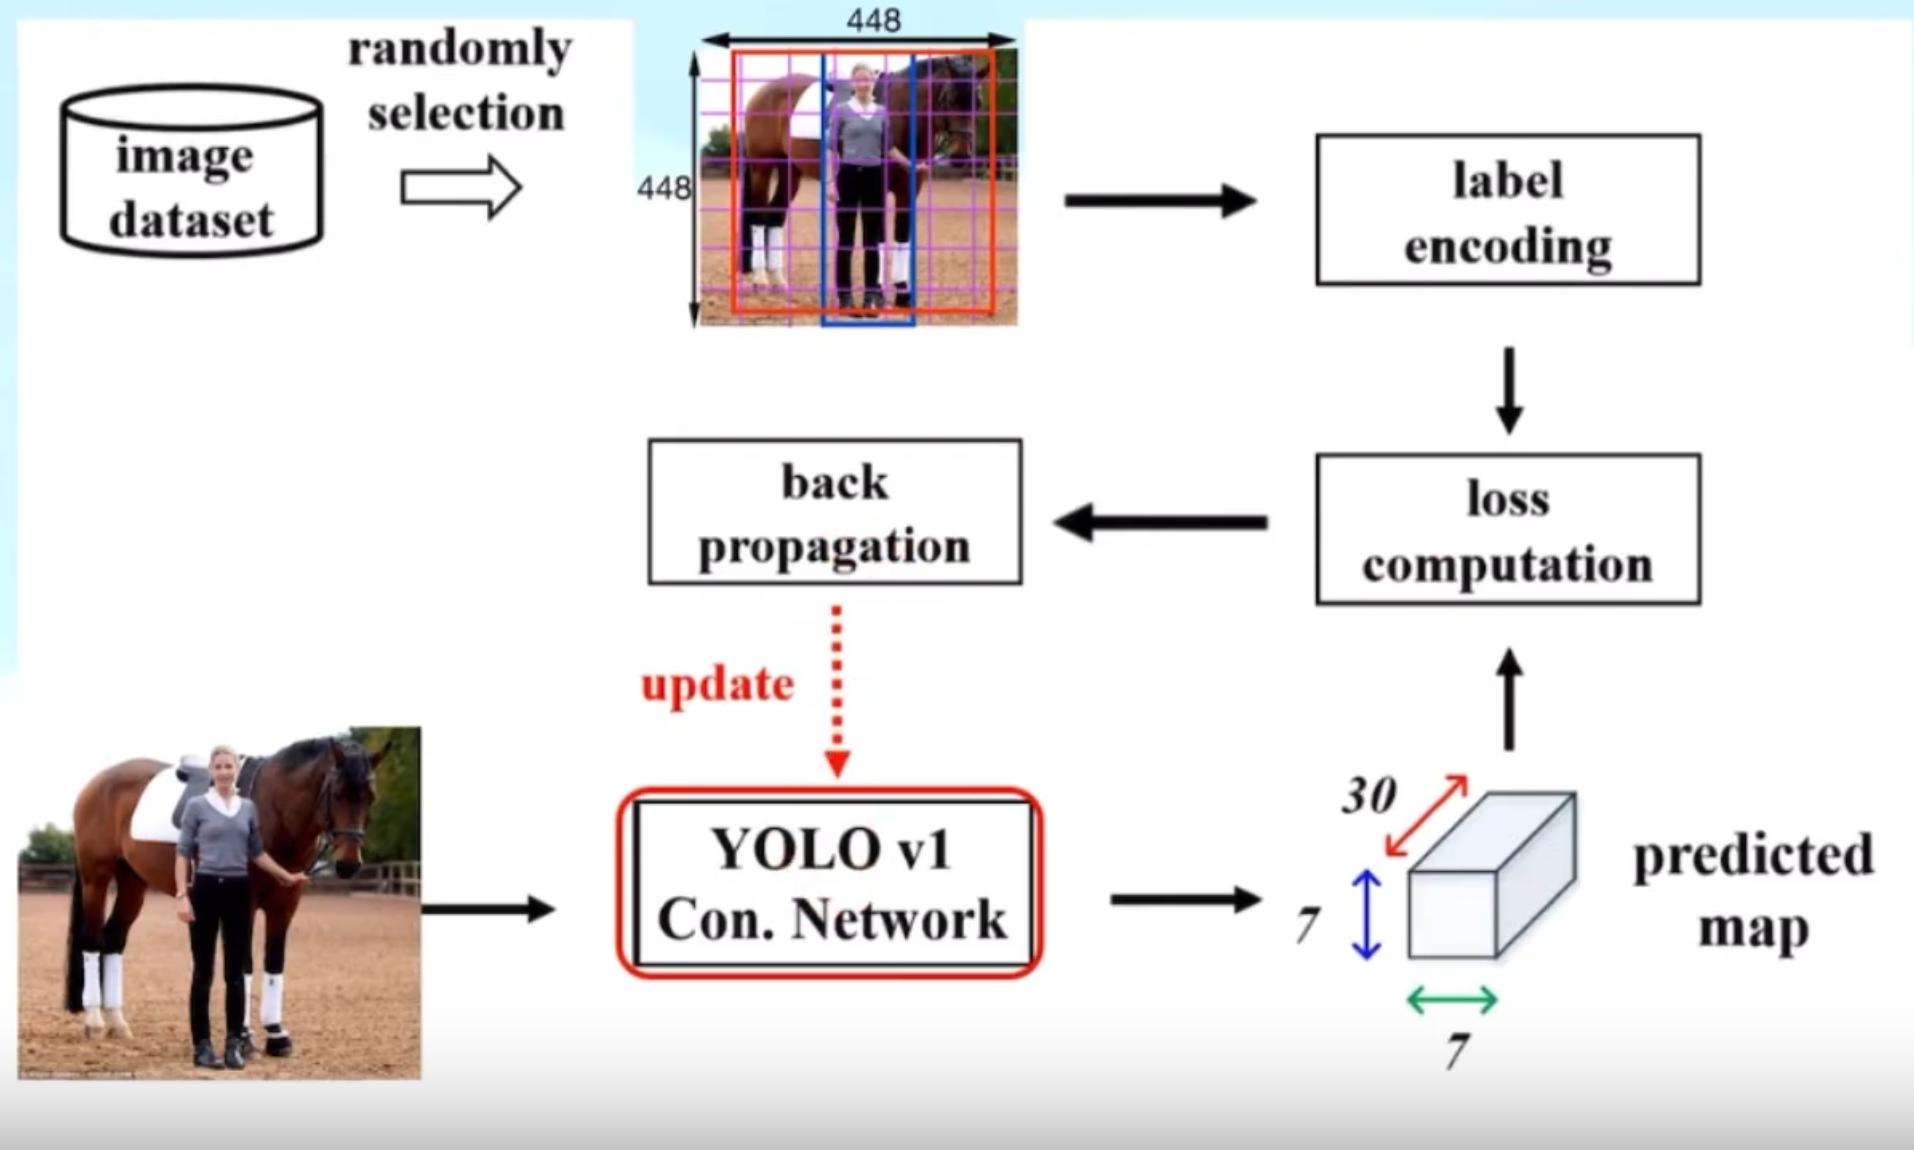
\includegraphics[width=0.8\linewidth]{images/yolo_train.png}
    \caption{\label{fig:yolo_train} Ilustração do processo de treinamento do \emph{YOLOv1}. Disponível em: \url{https://www.youtube.com/watch?v=zgbPj4lSc58&list=PL1u-h-YIOL0sZJsku-vq7cUGbqDEeDK0a&index=1&t=1517s}.}
\end{figure}

Escolhemos uma imagem aleatória do conjunto de dados, efetuamos o pré-processamento de seus rótulos como comentado, passamos a imagem pela rede neural, computamos a função de perda ao comparar os resultados do \emph{forward pass} com os rótulos processados e então efetuamos o processo de \emph{back propagation}, atualizando os pesos do modelo com base no gradiente da função de perda. 

\paragraph{Função de perda}
A função de perda introduzida pelo \emph{YOLOv1} é a soma das funções de perda por todas as \emph{grid cells}:
\begin{center}
\[
L = \sum_{i=1}^{S^2} L_i
\]
\end{center}
A função de perda é dividida nos casos em que o centro de um objeto está ou não localizado dentro de uma \emph{grid cell}. Isso é feito por meio das funções indicadoras $\mathds{1}_i^{\text{obj}}$ e $\mathds{1}_i^{\text{no\_obj}}$, que assumem respectivamente o valor 1 quando há e não há objetos na \emph{grid cell} $i$, e assumem 0 caso contrário. Além disso, desejamos dar mais importância para a presença de objetos na imagem, por isso, há a constante $\lambda_{\text{no\_obj}}$, que no artigo original tem o valor de 0,5:
\begin{center}
\[
L = \sum_{i=1}^{S^2} \mathds{1}_i^{\text{obj}} \cdot L_{i, \text{obj}} + \lambda_{\text{no\_obj}} \sum_{i=1}^{S^2} \mathds{1}_i^{\text{no\_obj}} \cdot L_{i, \text{no\_obj}}
\]
\end{center}

Agora, vamos definir $L_{i, \text{obj}}$. Essa função é definida como uma soma ponderada da função de perda da confiança de que há um objeto cujo centro está na \emph{grid cell} $i$ (\emph{objectness loss}), a função de perda da classificação e a função de perda das coordenadas da \emph{bounding box}.
\begin{center}
\[
L_{i, \text{obj}} = \lambda_{\text{coord}} \cdot L_{i, \text{obj}}^{\text{box}} + L_{i, \text{obj}}^{\text{conf}} + L_{i, \text{obj}}^{\text{cls}}
\]
\end{center}

No artigo original, $\lambda_{\text{coord}}$ tem o valor de 5.

A função de perda para as \emph{bounding boxes}, \( L_{i, \text{obj}}^{\text{box}} \), é definida como a soma dos erros quadráticos entre os valores preditos e os valores presentes no rótulo da imagem em questão (\emph{ground truth}). A expressão é dada por:

\[
L_{i, \text{obj}}^{\text{box}} = (\Delta x_i - \Delta \hat{x}_i)^2 + (\Delta y_i - \Delta \hat{y}_i)^2 + \left(\sqrt{\Delta w_i} - \sqrt{\Delta \hat{w}_i}\right)^2 + \left(\sqrt{\Delta h_i} - \sqrt{\Delta \hat{h}_i}\right)^2
\]

onde: \( \Delta x_i \) e \( \Delta y_i \) são as coordenadas reais do centro da \emph{bounding box};  \( \Delta \hat{x}_i \) e \( \Delta \hat{y}_i \) são as coordenadas preditas; \( \Delta w_i \) e \( \Delta h_i \) são a largura e a altura reais da \emph{bounding box}; e \( \Delta \hat{w}_i \) e \( \Delta \hat{h}_i \) são os valores preditos.

A raiz quadrada em \( w \) e \( h \) está presente na computação dessa função de perda pois, quanto maior a \emph{bounding box}, maiores serão as diferenças $\left(\Delta w_i - \Delta \hat{w}_i \right)$ e $ \left( \Delta h_i - \Delta \hat{h}_i \right)$. Esse aumento ocorre ainda mais ao usarmos o quadrado dessas diferenças. Por isso, a função de perda penaliza mais caixas maiores. Para tentar melhorar essa situação, a ideia é introduzir a raiz quadrada para diminuir a penalização de caixas de maior tamanho, já que maiores valores em $\left(\Delta w_i - \Delta \hat{w}_i \right)$ e $ \left( \Delta h_i - \Delta \hat{h}_i \right)$, após o uso da raiz quadrada, não impactarão tanto no valor final da função de perda.

Já a função de perda da confiança da presença de centro de objeto na \emph{grid cell} $i$, é somente o erro quadrático da confiança predita e do valor rótulo (nesse caso, sempre $1$).

\begin{center}
\[
L_{i, \text{obj}}^{\text{conf}} =  (c_i - \hat{c}_i)^2
\]
\end{center}

Por fim, a função de perda de classificação também é constituída por erro quadrático.

\begin{center}
\[
L_{i, \text{obj}}^{\text{cls}} = \sum_{c=1}^{20} (p_{i,c} - \hat{p}_{i,c})^2
\]
\end{center}

Em que $p$ e $\hat{p}$ são os vetores das probabilidades.

Agora, precisamos computar a função de perda no caso em que não há objetos cujo centro está localizado na \emph{grid cell} $i$. Nesse caso, somente levamos em consideração a \emph{objectness score}:

\begin{center}
\[
L_{i, \text{no\_obj}} = \sum_{j=1}^{B} (c_{i,j} - \hat{c}_{i,j})^2
\]
\end{center}

Em que o valor de $\hat{c}_{i,j}$ é 0 e $B$ igual a 2.

\paragraph{Limitações}
Apesar de ser uma arquitetura disruptiva que revolucionou o cenário da visão computacional e detecção de objetos, o \emph{YOLOv1} apresentava algumas limitações. Principalmente a incapacidade de detectar muitos objetos, principalmente quando os objetos são pequenos e estão amontoados. (limitação devido às \emph{grid cells}). Além disso, como todas as \emph{bounding boxes} têm sua origem em um processo adaptativo relativo às \emph{grid cells}, o \emph{YOLOv1} tem dificuldade em adaptar as caixas à objetos com proporções variadas \citep{yolo_review}.

\subsection{Métricas}
Para avaliar diferentes modelos de detecção de objetos, temos diversas métricas para quantificar a qualidade do modelo em identificar corretamente objetos em uma imagem. Vamos detalhar as métricas mais comuns, com base nas definições matemáticas do artigo \citep{Padilla2020A}.

\begin{itemize}
    \item {\bf \emph{Intersection over Union (IoU}:} 
    \emph{Intersection over Union} mede a área de sobreposição entre a \emph{bounding box} predita ($B_p$) e a \emph{bounding box} real (\emph{ground truth}) ($B_{gt}$).
    \begin{center}
        \[
        \text{IoU} = \dfrac{\text{Área}\left( B_p \cap B_{gt} \right)}{\text{Área}\left( B_p \cap B_{gt}\right)}
        \]
    \end{center}
    Uma das funções mais importantes dessa métrica é definir:
    \begin{itemize}
        \item Verdadeiros positivos (\emph{TP}): uma detecção correta de uma \emph{bounding box} real (\emph{ground-truth} \citep{Padilla2020A};
        \item Falsos positivos (\emph{FP}): uma detecção incorreta de um objeto inexistente ou uma detecção mal posicionada de um objeto existente \citep{Padilla2020A};
        \item Falsos negativos (\emph{FN}): uma \emph{bounding box} real (\emph{ground-truth}) não detectada \citep{Padilla2020A}.
    \end{itemize}

    Desse modo, consideramos a detecção correta de uma \emph{bounding box} caso a classe detectada seja a correta e $\emph{IoU} > t$.
    \item {\bf Precisão e \emph{Recall}:}
    A \emph{Precisão} (\(P\)) mede a proporção de predições corretas entre todas as predições feitas:
    \[
    P = \frac{\text{TP}}{\text{TP} + \text{FP}}
    \]

    O \emph{Recall} (\(R\)) mede a proporção de objetos reais detectados entre todos os objetos presentes na imagem:
    \[
    R = \frac{\text{TP}}{\text{TP} + \text{FN}}
    \]
    \item {\bf \emph{Average Precision (AP)}:}
    A \emph{Average Precision} (AP) é uma medida que combina a precisão e o \emph{recall}, calculando a área sob a curva de precisão-\emph{recall}. Primeiramente, precisamos entender como obtemos diversos valores de precisão e \emph{recall} para que seja possível traçar essa curva.
    
    Isso é feito ao escolhermos diversos valores $t$ do \emph{threshold} de confiança para classificação. Para cada valor de $t$, obtemos um par de valores de precisão e \emph{recall}. Depois disso, traçamos a curva. Então, um método comum para o cálculo do AP é a \textbf{interpolação em todos os pontos} \citep{Padilla2020A}:
    \[
    AP_{\text{all}} = \sum_{n} (R_{n+1} - R_n) P_{\text{interp}}(R_{n+1})
    \]
    onde onde
    \[
    P_{\text{interp}}(R_{n+1}) = \max_{\tilde{R} : \tilde{R} \geq R_{n+1}} P(\tilde{R}).
    \]
    Uma noção visual pode ser vista na figura \ref{fig:average_precision_curve}.
    \begin{figure}[htb!]
        \centering
        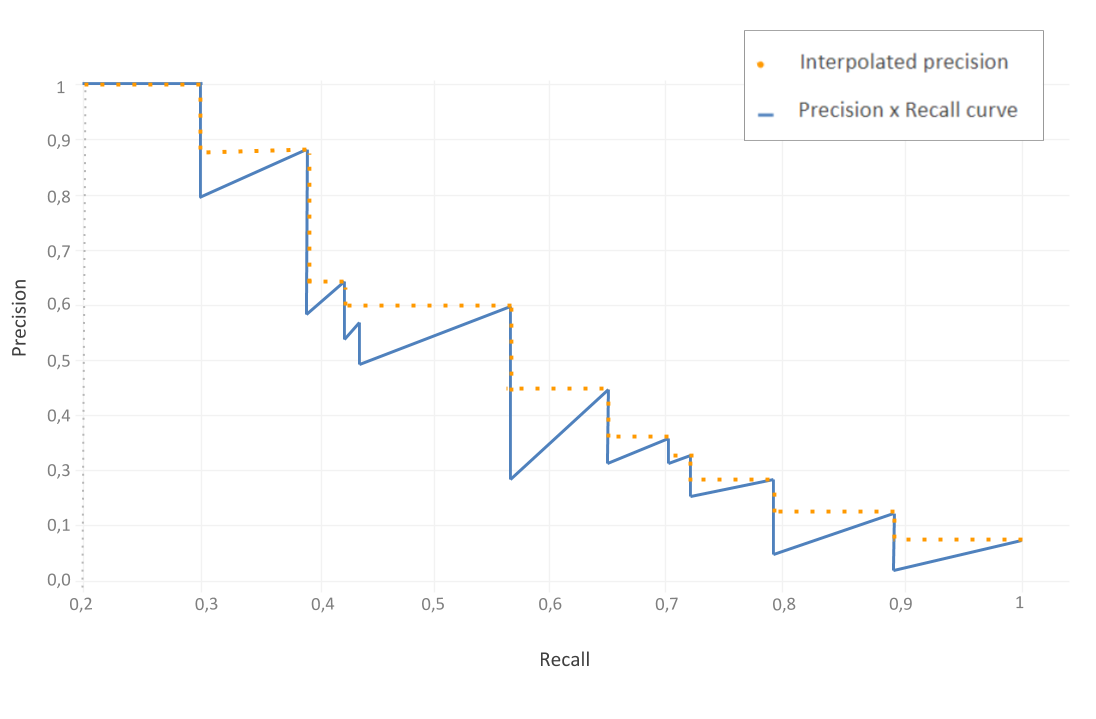
\includegraphics[width=0.8\linewidth]{images/ap.png}
        \caption{\label{fig:average_precision_curve} Exemplo de curva de precisão-\emph{recall} usando interpolação em todos os pontos para o cálculo da \emph{Average Precision (AP)}. Disponível em: \url{https://manalelaidouni.github.io/assets/img/pexels/all_point_interpolated_AP_(2)-848db820-1379-456f-bad8-8e45ea562fd0.png}.}
    \end{figure}
    
    \item {\bf \emph{Mean Average Precision (mAP)}:}
    A \emph{Mean Average Precision} (mAP) é a média do AP calculada sobre todas as classes em um conjunto de dados. Se um modelo é avaliado em \(N\) classes, a mAP é dada por:

    \[
    mAP = \frac{1}{N} \sum_{i=1}^{N} AP_i
    \]

    Onde \( AP_i \) é a AP para a classe \(i\).

\end{itemize}
Essas métricas, especialmente o AP e o mAP, são amplamente utilizadas para avaliar e comparar o desempenho de diferentes modelos de detecção de objetos. Além disso, há diferentes variantes do mAP para diferentes valores de IoU. Por exemplo, AP@50 (que gera a curva AP com o valor de $t$ em 0,5); AP@75 e AP@50:5:95, que entrega diversos valores.

\subsection{Avanços da família \emph{YOLO}}
\paragraph{\emph{Backbone}, \emph{neck} e \emph{head}:}
Com o avanço das arquiteturas para detecção de objetos, nomenclaturas para diferentes partes das redes neural convolucionais começaram a ser 
utilizadas. Nesse contexto, se destacam o {\bf backbone}, {\bf neck} e {\bf head}. Por isso, como parte da explicação sobre a evolução da família \emph{YOLO}, é interessante abordar a função de cada uma dessas partes dos detectores de objetos.

\begin{figure}[htb!]
    \centering
    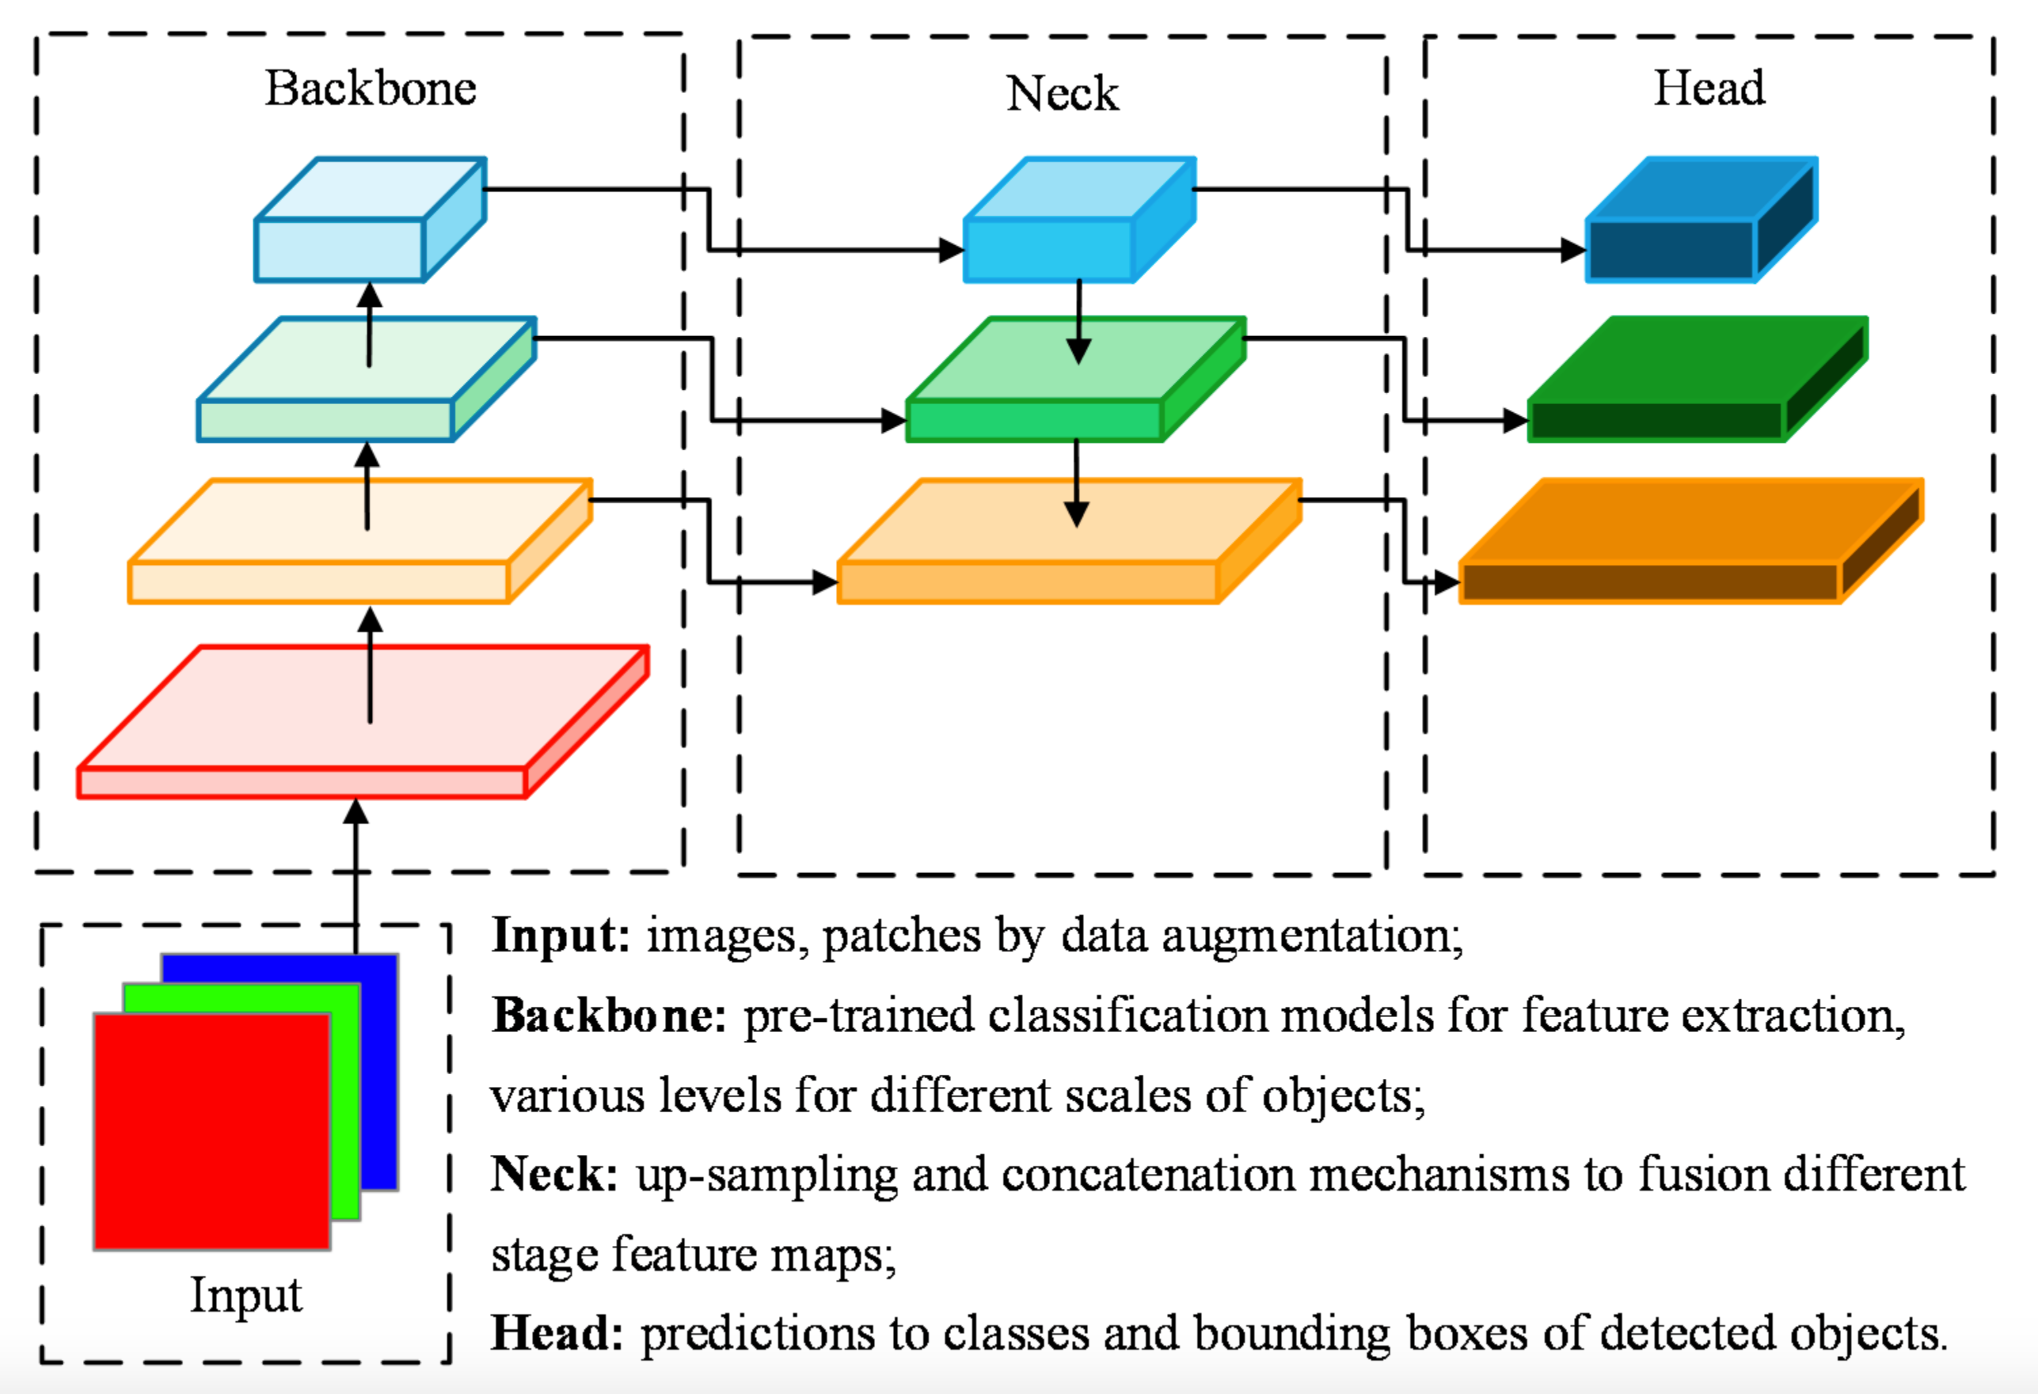
\includegraphics[width=0.8\linewidth]{images/backbone-neck-head.png}
    \caption{\label{fig:backbone_neck_head} Estrutura de detecção de objetos mostrando a separação entre \emph{Backbone}, \emph{Neck} e \emph{Head}. Disponível em: \url{https://velog.io/@peterkim/Object-Detection에서-말하는-Backbone-Neck-Head}.}
\end{figure}

\begin{itemize}
    \item {\bf Backbone:} o \emph{backbone} da rede convolucional, muitas vezes referido como uma rede em si, é muito comum em arquiteturas de modelos de detecção de objetos. A função do \emph{backbone} é realizar a extração das representações da imagem. Além disso, essas características extraídas são codificadas em uma dimensão adequada para o \emph{neck}, que será explicado a seguir. O \emph{backbone} deve ser capaz de capturar representações de alto nível e baixo nível da imagem de entrada \citep{shroff2021know}.
    
    \item {\bf Neck:} depois do \emph{backbone}, o \emph{neck} é responsável por transformar ainda mais as representações que foram extraídas anteriormente. O seu objetivo é melhorar a qualidade dessas representações de modo que elas sejam capazes de fornecer ainda mais informação para a detecção de objetos \citep{shroff2021know}.

    \item {\bf Head:} a \emph{head} do modelo de detecção de objetos é a sua parte final. Ela é responsável por produzir as predições do modelo e se baseia nas informações extraídas pelo \emph{backbone} e \emph{neck} \citep{shroff2021know}.
\end{itemize}

\paragraph{Abordagem baseada em âncoras:}
Desde o lançamento do \emph{YOLOv1}, a abordagem para detecção de objetos evoluiu significativamente. As versões subsequentes introduziram conceitos importantes, como o uso de \emph{âncoras} (\emph{anchors}) no \emph{YOLOv2} e \emph{YOLOv3}. As âncoras são \emph{bounding boxes} predefinidas que servem como referências para o modelo detectar objetos de diferentes escalas e proporções. Isso é feito geralmente utilizando o algoritmo de clusterização não supervisionado \emph{K-means} nas \emph{bounding boxes} presentes nos dados de treinamento do modelo de detecção. Essa técnica melhorou a precisão na detecção, mas adicionou complexidade ao processo \citep{yolo_review}.

\paragraph{\emph{YOLOX}:}
Com o surgimento do \emph{YOLOX} \cite{yolox2021}, foi adotada uma abordagem \emph{anchor-free}, eliminando a necessidade de âncoras predefinidas. Em vez disso, o modelo efetua a regressão das \emph{bounding boxes} diretamente pela \emph{CNN}, simplificando o processo de detecção. Além disso, o \emph{YOLOX} introduziu à família de modelos \emph{YOLO} a abordagem de uma \emph{head} desacoplada, ou seja: cada ``parte'' (\emph{branch}) da \emph{CNN} poderia se especializar na sua tarefa (uma delas na regressão das \emph{bounding boxes} e a outra na tarefa de classificação). Nesse ponto, a tarefa de detecção de objetos na arquitetura \emph{YOLO} deixou de ser uma tarefa centrada em regressão e passou a ser uma tarefa desacoplada de classificação e regressão \citep{yolox2021}. De qualquer forma, é interessante ressaltar que, apesar do desacoplamento, o treinamento é feito de maneira única. Com uma só passagem da imagem pela rede neural, obtemos todos os resultados da tarefa de detecção de objetos, o que não retorna à abordagem tradicional (de detecção em múltiplas etapas).

\paragraph{\emph{YOLOv8:}}
O \emph{YOLOv8}, desenvolvido pela \emph{Ultralytics} e lançado em janeiro de 2023 \citep{yolov8_2023}, incorporou essa abordagem \emph{anchor-free} e introduziu diversas melhorias na arquitetura:

\begin{itemize} 
    \item \textbf{Melhorias no \emph{backbone} e \emph{neck}}: O \emph{YOLOv8} utiliza um \emph{backbone} mais eficiente para extração de representações, aliado a um \emph{neck} aprimorado que facilita a fusão de informações de múltiplas escalas. Isso melhora a capacidade do modelo em detectar objetos de diferentes tamanhos, especialmente objetos pequenos em imagens de alta resolução;

    \item \textbf{Desacoplamento da \emph{head}}: De modo semelhante ao \emph{YOLOX}, o \emph{YOLOv8} implementa uma \emph{head} desacoplada, onde as tarefas de regressão das \emph{bounding boxes} e de classificação são realizadas de forma separada. Essa separação permite otimizar cada tarefa individualmente, aumentando a precisão geral do modelo.

    \item \textbf{Funções de perda específicas}: No processo de treinamento, o modelo utiliza uma combinação de \emph{Complete Intersection over Union} (CIoU) \citep{Zheng2020} e \emph{Distribution Focal Loss} (DFL) \citep{Li2020} na função de perda da regressão das \emph{bounding boxes}. Para a perda de classificação, é empregada a \emph{Binary Cross-Entropy} (BCE). Essa abordagem especializada para cada tipo de perda contribui para melhorias significativas na precisão da detecção \citep{yolo_review}.
\end{itemize}
\begin{figure}[htb!]
    \centering
    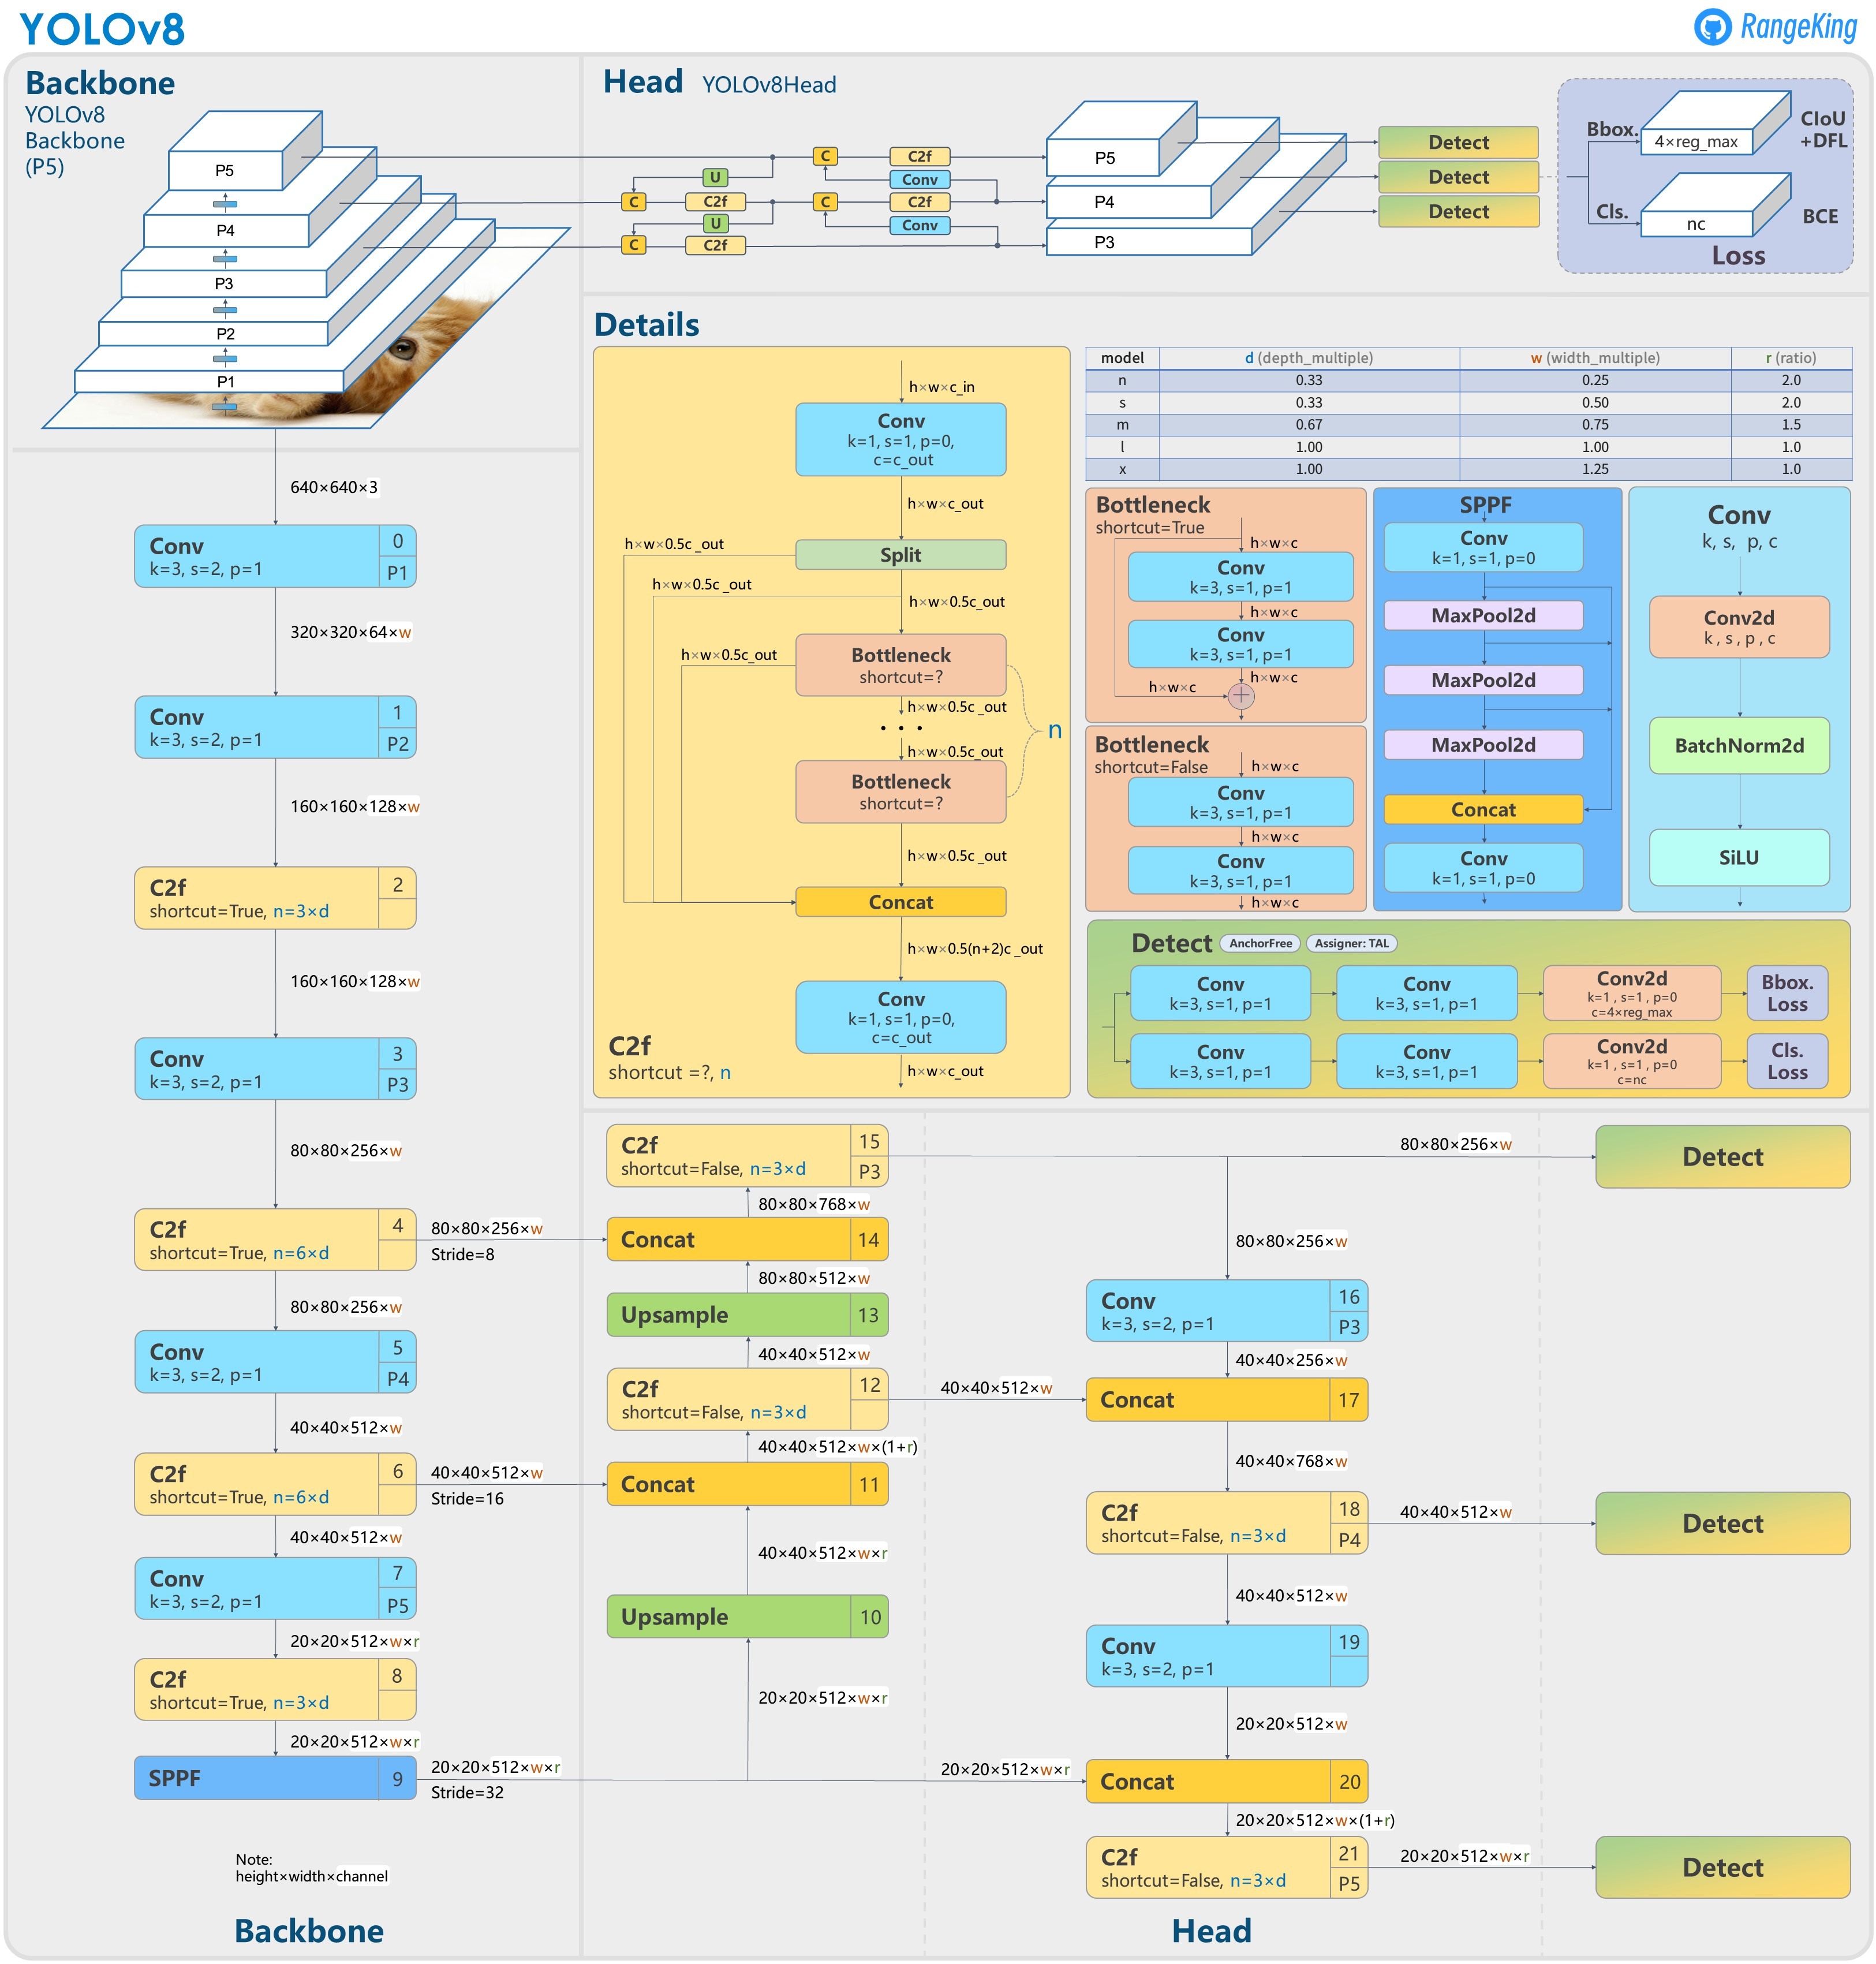
\includegraphics[width=0.8\linewidth]{images/yolov8.jpg}
    \caption{\label{fig:yolov8_issue189} Figura que ilustra a arquitetura do \emph{YOLOv8}. Imagem extraída de \citeauthor{ultralytics_issue_189}. Disponível em: \url{https://github.com/ultralytics/ultralytics/issues/189}.}
\end{figure}

Essas inovações resultaram em um desempenho superior do \emph{YOLOv8} em comparação com suas versões anteriores. Em testes realizados no conjunto de dados COCO, o \emph{YOLOv8} demonstrou um aumento no \emph{Mean Average Precision} (mAP) e uma velocidade de inferência mais rápida \citep{ultralytics_yolov8_results}.

Infelizmente, não houve a publicação de um artigo científico oficial da \emph{Ultralytics} para que possamos saber com facilidade o passo a passo do funcionamento do modelo \emph{YOLOv8}. Além disso, o repositório do \emph{Github} que contém a codificação da arquitetura do modelo está passando por atualizações constantes, com as modificações do código fonte do \emph{YOLOv8} para novos códigos, que originaram o \emph{YOLO11}. Dessa forma, consideramos que a profundidade da explicação feita sobre o \emph{YOLOv8} é o bastante para o intuito desse trabalho de formatura supervisionado.


\section{Materiais e métodos}
\label{sec:treinamento}
Depois de escolhermos o modelo \emph{YOLOv8} para realizar a detecção de objetos no projeto \emph{TomatoHealth}, chegou o momento de treiná-lo para que ele tivesse a capacidade de detectar as doenças em folhas de tomate. Como comentado anteriormente, o \emph{dataset} escolhido para essa tarefa foi o \emph{PlantDoc}, mas com o escopo reduzido para doenças em folhas de tomate.

\subsection{Processamento do \emph{dataset}}
Para obtermos o \emph{dataset} das doenças em folhas de tomate, precisamos então realizar uma filtragem no \emph{PlantDoc} para que somente imagens que possuam rótulos de doenças de tomate (e esses rótulos em si) permanecessem na versão do \emph{dataset} que seria utilizada para treinar o modelo.

Para fazer isso, primeiro obtemos o conjunto de dados \emph{PlantDoc} a partir da plataforma \emph{Dataset Ninja}\footnote{\url{https://datasetninja.com/plantdoc}} --- essa plataforma disponibiliza conjuntos de dados para uso em projetos de \emph{Machine Learning}. Depois disso, no processo de filtragem do \emph{dataset}, também precisamos fazer adaptações no formato dos \emph{rótulos} e da estrutura de diretórios para que tivéssemos um conjunto de dados adaptado para a arquitetura \emph{YOLO}.

Sobre os rótulos, o formato inicial define as \emph{bounding boxes} a partir do seu vértice superior esquerdo e do seu vértice inferior direito. Então precisamos fazer uma transformação para obter o tamanho, largura e centro de cada caixa. O código responsável por esse processamento pode ser encontrado no repositório de códigos do projeto\footnote{\url{https://github.com/heitorc62/TCC}}.

Inicialmente, a estrutura de diretórios apresentava o seguinte formato:
\begin{verbatim}
treino/
|-- imgs/
|-- rótulos/
teste/
|-- imgs/
|-- rótulos/
\end{verbatim}
Para o uso com o \emph{YOLO}, a organização de diretórios precisa ser ajustada para separar as imagens e os rótulos em diretórios específicos, com subdiretórios para treino e teste. A estrutura correta é:
\begin{verbatim}
imgs/
|-- treino/
|-- teste/
rótulos/
|-- treino/
|-- teste/
\end{verbatim}
Ao final de todo esse processamento, restaram as seguintes classes no \emph{dataset}:

\begin{table}[h!]
\centering
\resizebox{\textwidth}{!}{
\begin{tabular}{|c|l|l|}
\hline
\textbf{ID} & \textbf{Nome Original (Inglês)} & \textbf{Nome em Português} \\
\hline
0 & Tomato Early blight leaf & Folha de tomate com pinta-preta \\
1 & Tomato leaf & Folha de tomate saudável \\
2 & Tomato leaf bacterial spot & Folha de tomate com mancha bacteriana \\
3 & Tomato leaf late blight & Folha de tomate com requeima \\
4 & Tomato leaf mosaic virus & Folha de tomate com vírus do mosaico \\
5 & Tomato leaf yellow virus & Folha de tomate com Begomovirus (yellow leaf curl virus) \\
6 & Tomato mold leaf & Folha de tomate com mofo \\
7 & Tomato Septoria leaf spot & Folha de tomate com septoriose (fungo) \\
8 & Tomato two spotted spider mites leaf & Folha de tomate com ácaro-rajado (spider mite) \\
\hline
\end{tabular}
}
\caption{Nomes originais das classes e suas traduções em português.}
\label{tab:class-names}
\end{table}

\begin{figure}[htb!]
    \centering
    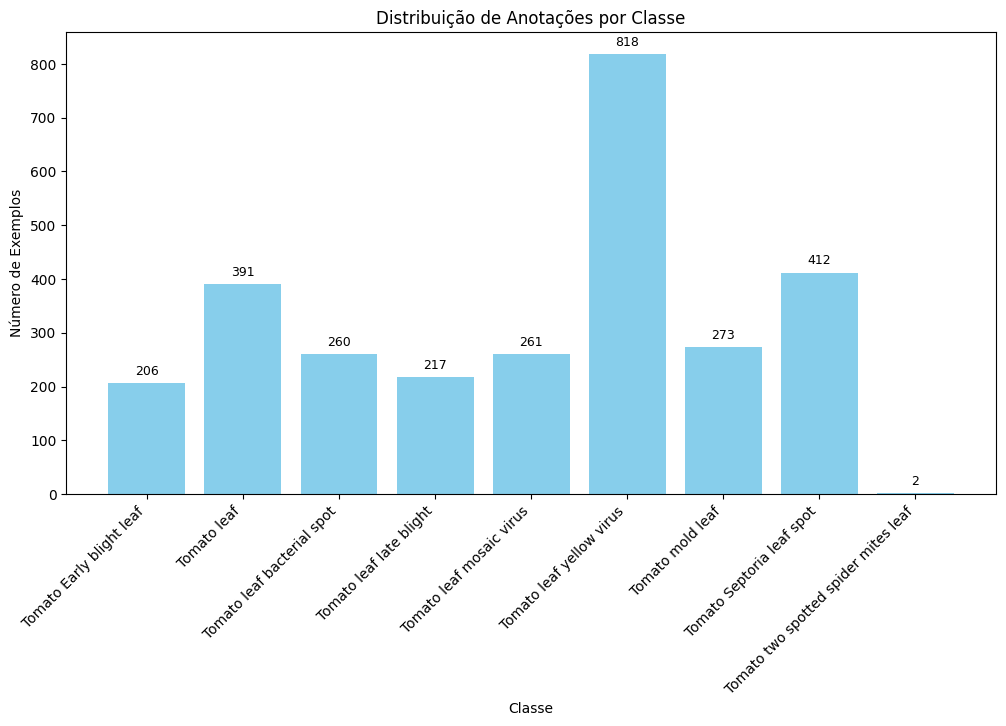
\includegraphics[width=1\linewidth]{images/distribuicao_anotacoes.png}
    \caption{\label{fig:distribuicao-ann-cls} Gráfico de barras mostrando a distribuição de anotações por classe após o processamento do conjunto de dados \emph{PlantDoc}. Fonte: acervo dos autores.}
\end{figure}

Totalizando 721 imagens, 2840 anotações e uma média de 3.93897 anotações por imagem. Na figura \ref{fig:distribuicao-ann-cls} é possível enxergar a distribuição de anotações por classes. É notável que a classe \emph{Tomato two spotted spider mites leaf} possui um número muito pequeno de exemplos. Contudo, como o intuito do projeto é, justamente estender o atual conjunto de dados com novas imagens e novas anotações, decidimos não desconsiderar essa classe e mantê-la no conjunto de dados.

\subsection{Treinamento}
\label{sec:treinamento2}
Após o pré-processamento, o conjunto de dados foi adequadamente estruturado para ser utilizado pelo \emph{YOLO}. Com isso, o próximo passo foi realizar o treinamento do modelo. Executamos um processo de ajuste fino (\emph{fine-tuning}) do \emph{YOLOv8n} (uma versão mais leve do \emph{YOLOv8}), previamente treinado no \emph{dataset} COCO\footnote{\url{https://yolov8.org/yolov8-coco-dataset/}} \cite{COCO}.

Para realizar o ajuste fino, foram utilizadas duas abordagens principais:

\begin{itemize}
    \item \textbf{Linha de comando com \emph{Bash}}: A primeira opção é rodar o treinamento diretamente no terminal com um comando \emph{bash}, que especifica configurações, como a tarefa, o número de épocas e o tamanho da imagem:

\begin{lstlisting}
    yolo task=detect mode=train model=yolov8n.pt data=tomato.yaml epochs=300 imgsz=640 device=0 
\end{lstlisting}

   \begin{itemize}
       \item \texttt{task=detect}: define a tarefa como detecção de objetos.
       \item \texttt{model=yolov8n.pt}: indica o modelo \emph{YOLOv8} pré-treinado a ser utilizado.
       \item \texttt{data=tomato.yaml}: aponta para o arquivo de configuração dos dados, que mapeia as classes para seus nomes e os caminhos das imagens.
       \item \texttt{epochs=50}: número de épocas para o treinamento.
       \item \texttt{imgsz=640}: define o tamanho das imagens usadas no treinamento.
       \item \texttt{device=0}: especifica o dispositivo (\emph{GPU}) para acelerar o treinamento.
   \end{itemize}

    \item \textbf{Uso da biblioteca \emph{Python} da \emph{Ultralytics}}: A segunda opção é utilizar funções disponibilizadas pela biblioteca de \emph{Python} da \emph{Ultralytics}:
    \begin{lstlisting}
       results = model.train(task="detect", data=data_yaml, epochs=epochs, imgsz=img_size, device=device)
    \end{lstlisting}
\end{itemize}
Para treinar o modelo, utilizamos a rede de computadores (\emph{vision, e-science}) com placas de vídeo (\emph{GPU}). Mais especificamente a máquina chamada \emph{deepthree}, com 200\emph{GB} de RAM e equipada com a placa de vídeo \emph{NVIDIA GeForce GTX 1080 Ti} com 12\emph{GB} de memória.

\subsection{Resultados}
\label{sec:resultados}
Com o \emph{dataset} que obtivemos após o processamento e utilizando o \emph{YOLOv8n}, decidimos fazer um treinamento por 300 épocas. As ferramentas fornecidas pela \emph{Ultralytics} facilitam muito esse processo. O parâmetro \emph{EarlyStopping(patience=100)} define que o treinamento para após 100 épocas sem melhorias nas métricas de avaliação. Então, após 183 épocas o treinamento foi finalizado já que o melhor modelo encontrado foi do final da época de número 83. O treino com 183 épocas e utilizando as configurações de hardware mencionadas na seção \ref{sec:treinamento2}, leva cerca de 30 minutos e resulta em um arquivo de pesos de cerca de 6\emph{MB}. Os resultados obtidos podem ser vistos na figura \ref{fig:resultados-treinamento}.

\begin{figure}[htb!]
    \centering
    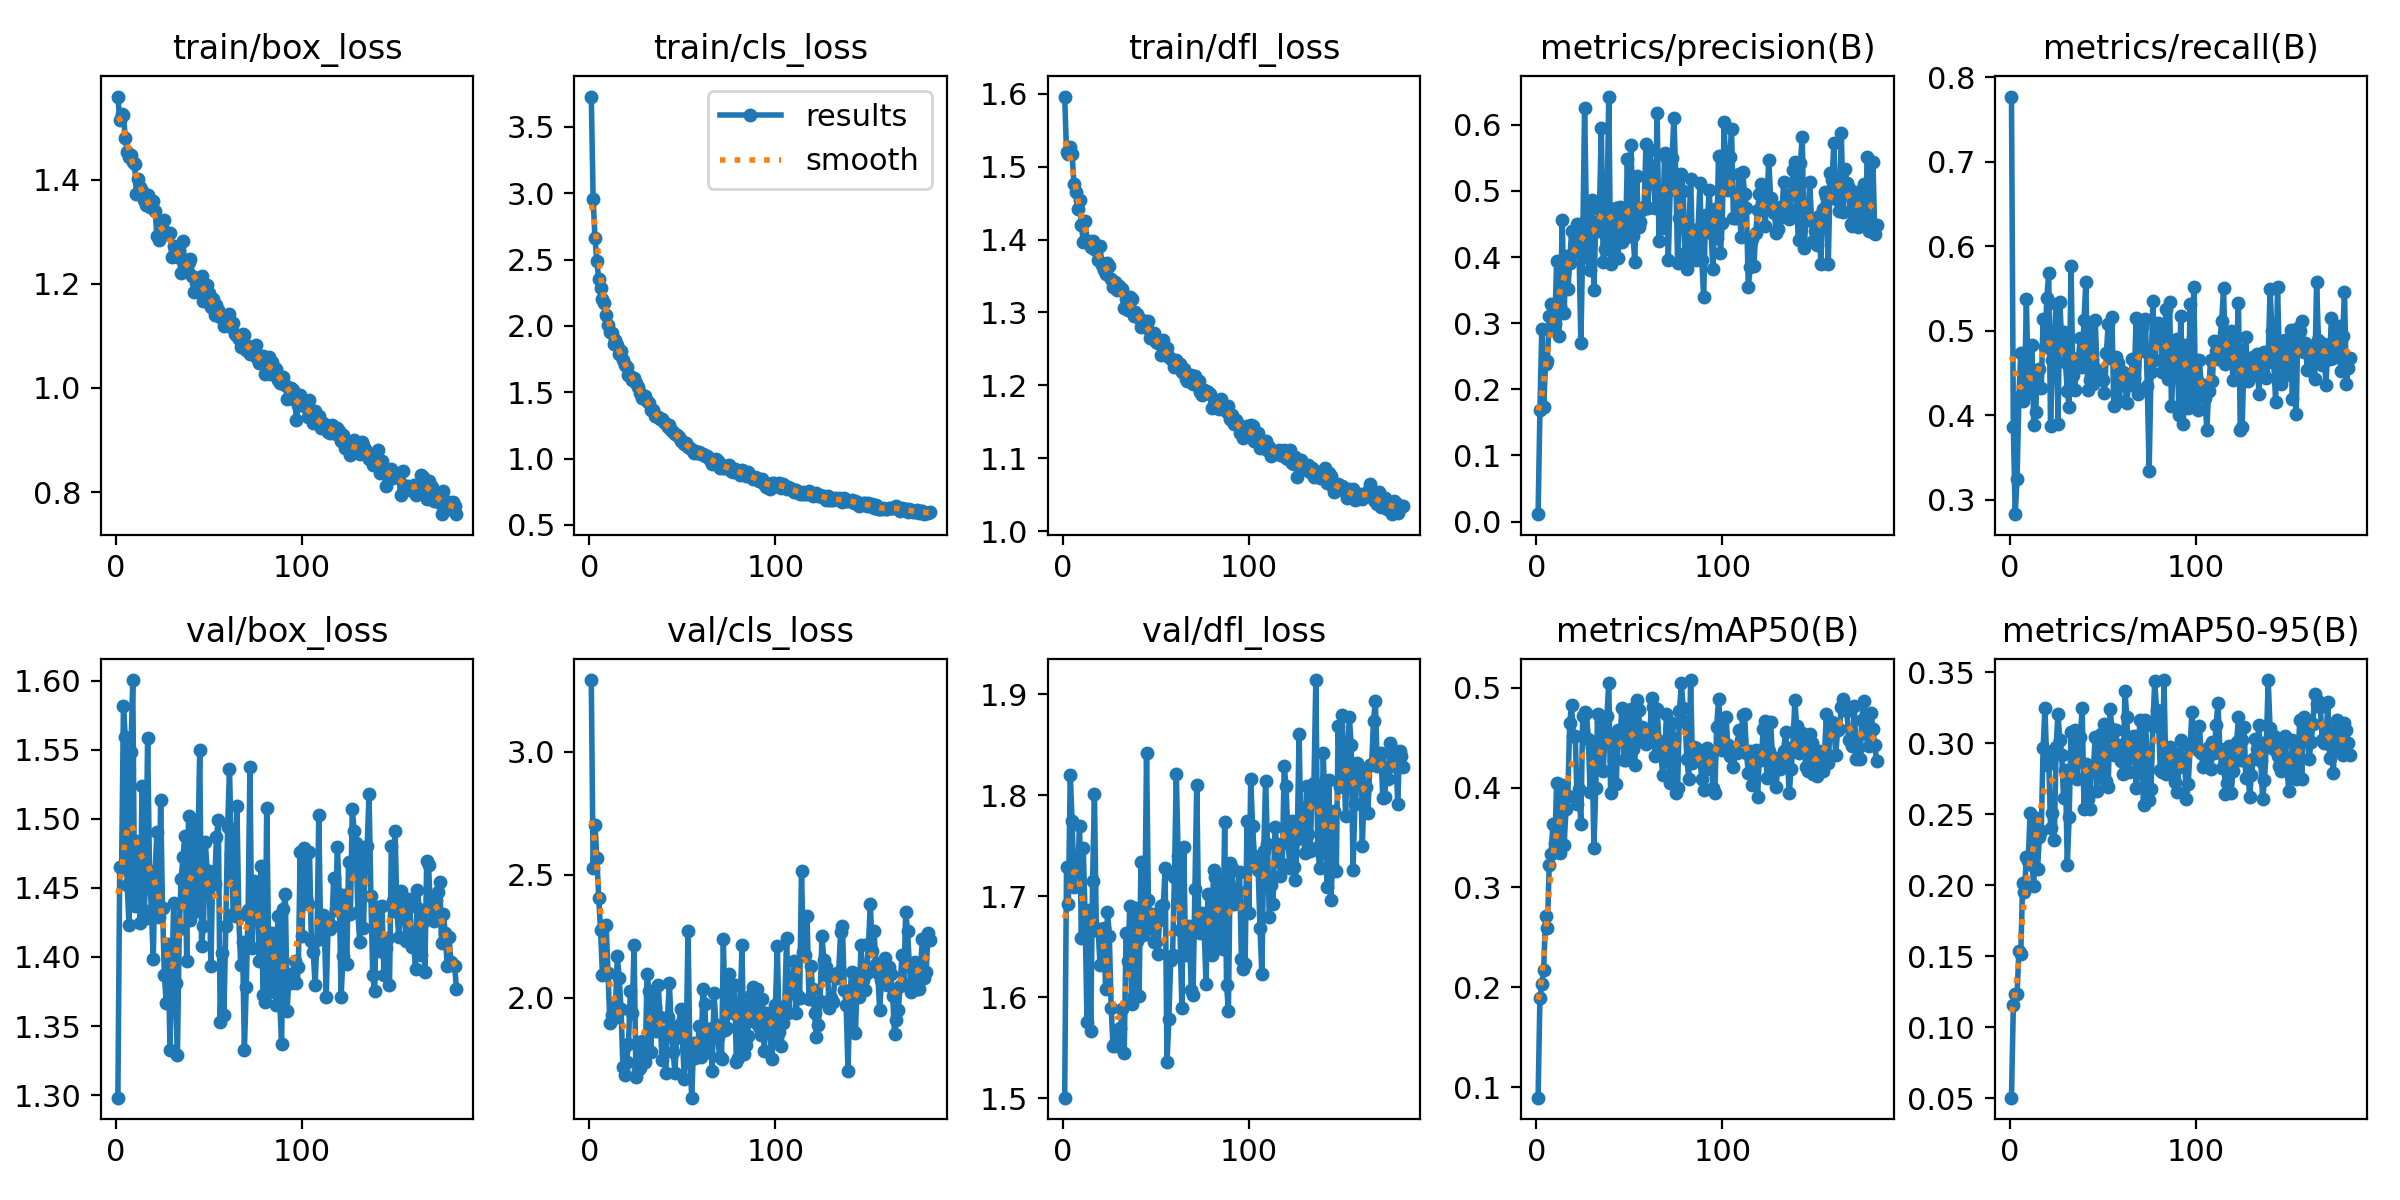
\includegraphics[width=1\linewidth]{images/results.png}
    \caption{Resultados obtidos após 183 épocas de treinamento. Fonte: acervo dos autores.}
    \label{fig:resultados-treinamento}
\end{figure}

O melhor valor da métrica \emph{mAP\string@50-95} obtido após o treinamento foi: 34,437; Se compararmos esse valor com os melhores resultados do \emph{YOLOv8} na referência de performance do \emph{dataset COCO} (37.3) conseguimos notar que, pelo menos na teoria, o conjunto de dados está performando bem.

Apesar do intuito do \emph{TomatoHealth} ser a construção de um conjunto de dados robusto no domínio de detecção de doenças em folhas de tomate, pensamos que em um momento inicial é interessante ter um modelo que seja o melhor possível. 

Assim, devido ao pequeno número de exemplos que possuímos inicialmente nesse \emph{dataset}, reconhecemos que essa métrica de 34,437 pode estar superestimada e isso pode ser observado nas figuras \ref{fig:val-pred} e \ref{fig:val-labels} (predições incorretas no conjunto de validação). Então, consideramos uma estratégia para tentar melhorar essa performance inicial. Essa estratégia será discutida na seção \ref{sec:integrando-resultados}.
\begin{figure}[H]
    \centering
    \begin{subfigure}[t]{0.45\textwidth}
        \centering
        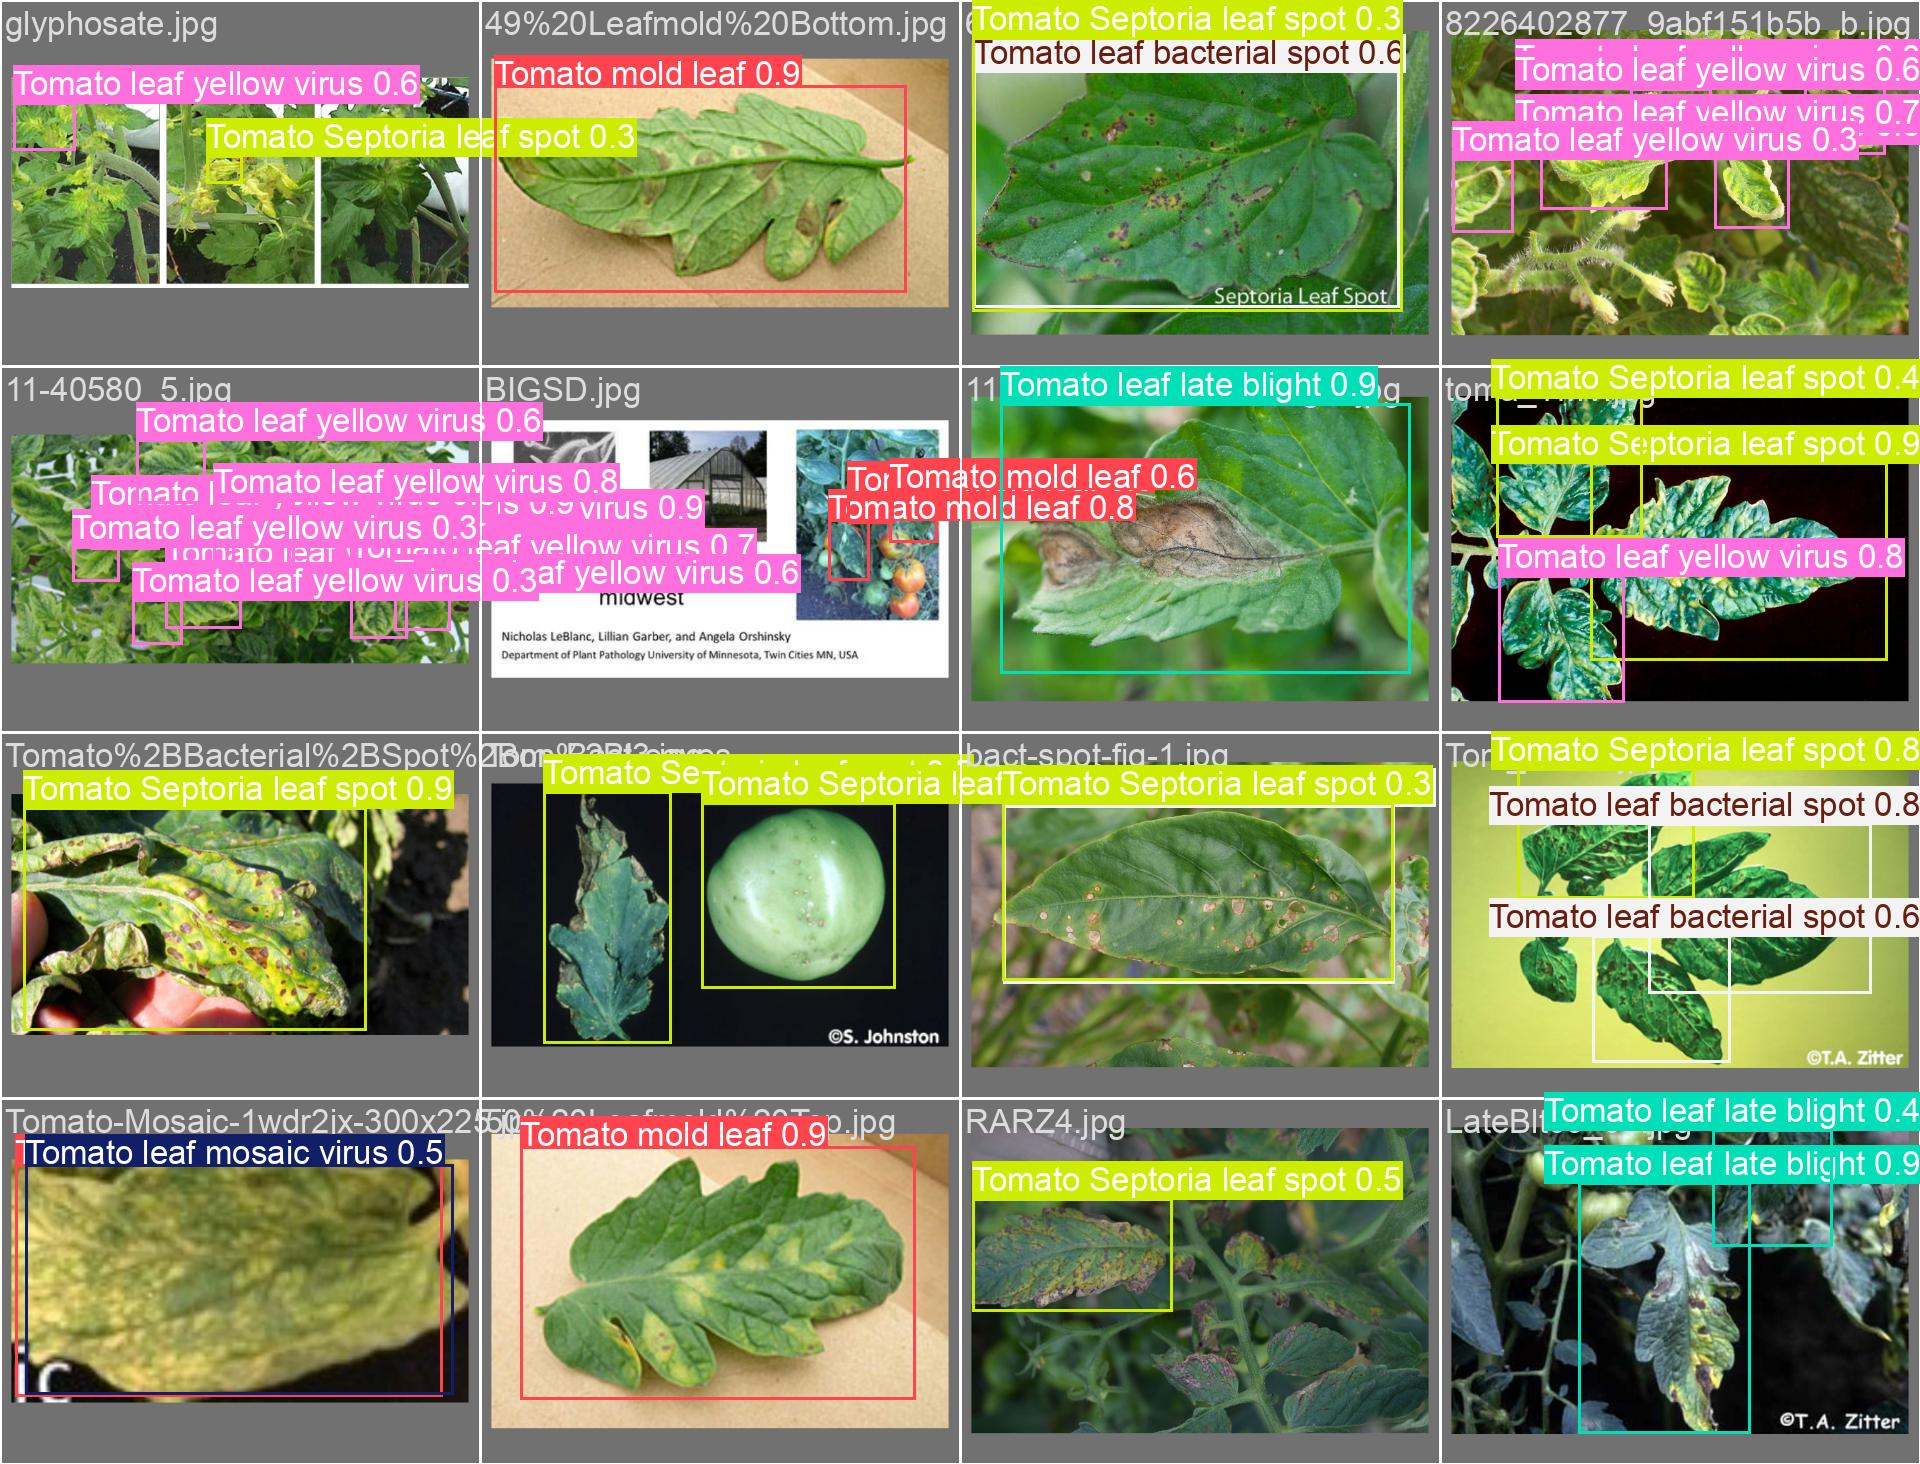
\includegraphics[width=\textwidth]{images/val_batch0_pred.jpg}
        \caption{Exemplo de deteccao de objetos em imagens do conjunto de validação. Imagem extraída do acervo dos autores.}
        \label{fig:val-pred} 
    \end{subfigure}\hfill
    \begin{subfigure}[t]{0.45\textwidth}
        \centering
        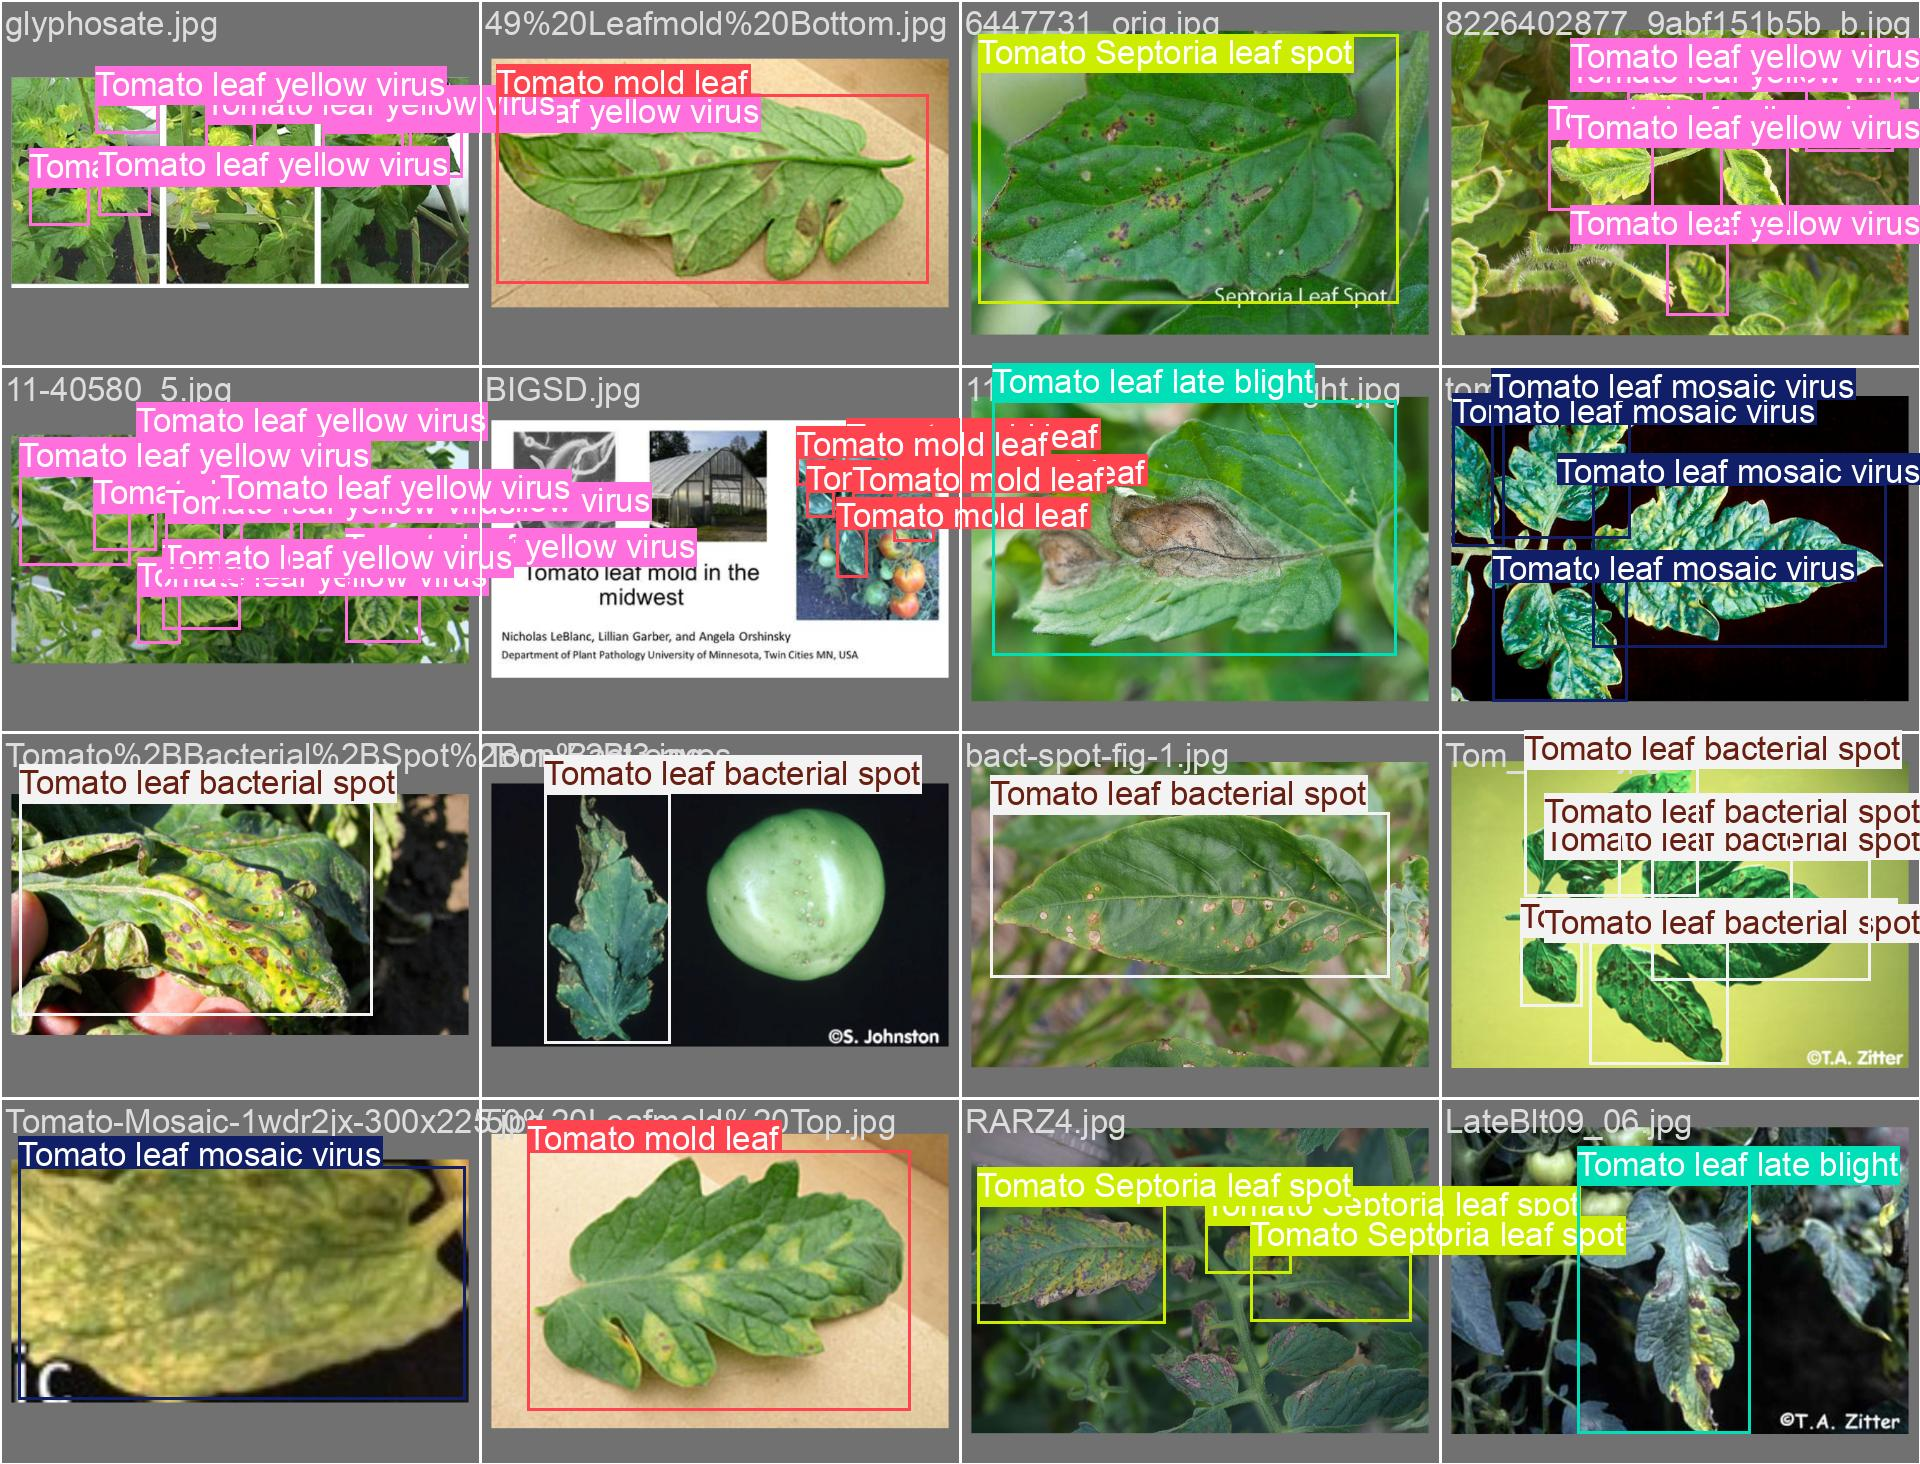
\includegraphics[width=\textwidth]{images/val_batch0_labels.jpg}
        \caption{Exemplo de rotulos de objetos. Imagem extraída do acervo dos autores.}
        \label{fig:val-labels}
    \end{subfigure}
    \caption{Comparação entre a detecção de objetos e os rotulos originais.}
    \label{fig:comparison}
\end{figure}
\chapter{Detalhes sobre a implementação do sistema} \label{sec:implementacao_sistema}

Nesse capítulo, apresentaremos detalhes técnicos sobre a implementação do sistema \textit{TomatoHealth}, tecnologias utilizadas e decisões do desenvolvimento tomadas para um sistema com as capacidades do descrito no capítulo \ref{sec:abst-det}.

\section{Arquitetura cliente-servidor e contêineres \emph{Docker}}

O \emph{TomatoHealth} implementa uma arquitetura de cliente-servidor, com dois tipos de clientes diferentes: clientes de usuários comuns e de especialistas, que se diferenciam conforme os requisitos do capítulo \ref{sec:abst-geral}.

Do ponto de vista da arquitetura cliente-servidor e da descrição abstrata para o usuário geral, os tópicos de mais difícil implementação são: tirar, enviar e receber uma foto para análise; já que entender o papel da ferramenta é uma tarefa do \emph{front-end}. Para realizar essas tarefas difíceis, o cliente faz uma requisição \emph{POST HTTP} enviando uma imagem com o uso da \emph{API FormData}\footnote{\url{https://developer.mozilla.org/en-US/docs/Web/API/FormData}}. E por sua vez, o servidor salva essa imagem no banco de dados \emph{S3 MinIO}, realiza a detecção das classes presentes, faz um prompt para a \emph{LLM} \texttt{gpt-4o-mini} da \emph{OpenAI} por \emph{API}\footnote{\url{https://platform.openai.com/docs/api-reference/introduction}} (pergunta ao modelo como tratar um tomateiro com as doenças detectadas) e finalmente responde o \emph{POST} do cliente com o \emph{output} da \emph{LLM}.

Já para o cliente especialista, as tarefas de ver as imagens tiradas por usuários comuns e demarcar as diferentes classes são solucionadas com a utilização da ferramenta de anotação \emph{Label Studio}. Essa ferramenta já inclui uma interface de rotulagem de dados que se comunica com o banco onde essas imagens são guardadas, e ela pode ser facilmente alterada para os propósitos da nossa aplicação.

Um modelo simples para nossa arquitetura pode ser visto na figura \ref{fig:modelo_arq}.

\begin{figure}[htbp]
    \centering
    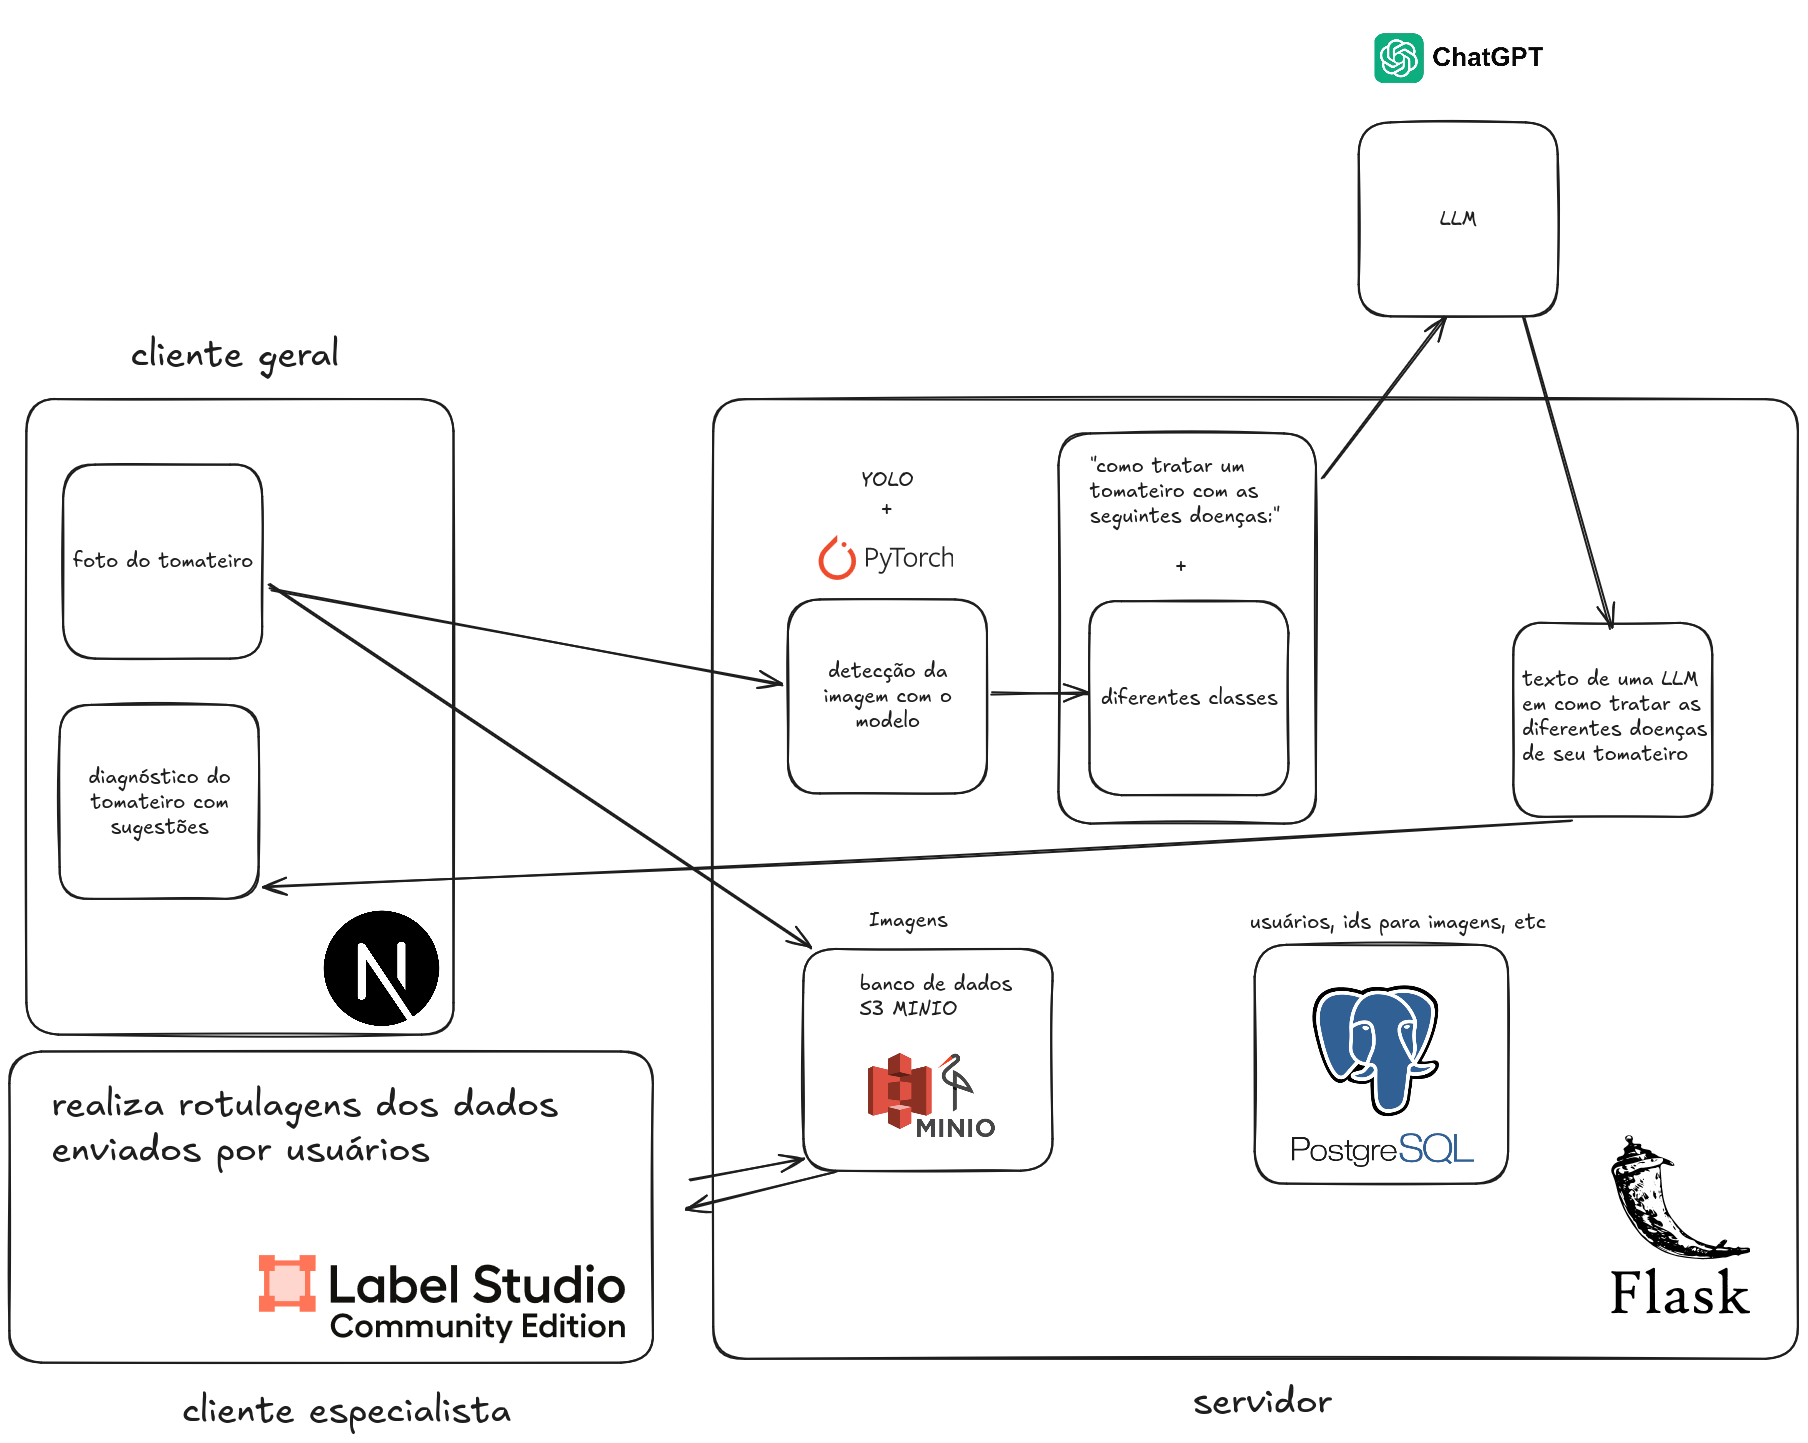
\includegraphics[width=1\linewidth]{images/modelo.png}
    \caption{\label{fig:modelo_arq} Modelo simples para a arquitetura implementada. A imagem apresenta as logos das tecnologias usadas: ChatGPT, Next.js, Label Studio, MinIO, PostgreSQL e Flask. Fonte: acervo dos autores.}
\end{figure}

Além disso, utilizamos contêineres \emph{Docker} \footnote{\url{https://www.docker.com/}}, pois facilitam o processo de desenvolvimento, uma vez que lidamos com o uso de diferentes \textit{frameworks} e bancos de dados, além de utilizarmos a ferramenta \emph{Docker Compose} para o controle de inicialização, execução e comunicação entre os contêineres. A figura \ref{fig:containers} demonstra os diferentes contêineres de nossa aplicação.

\begin{figure}[htbp]
    \centering
    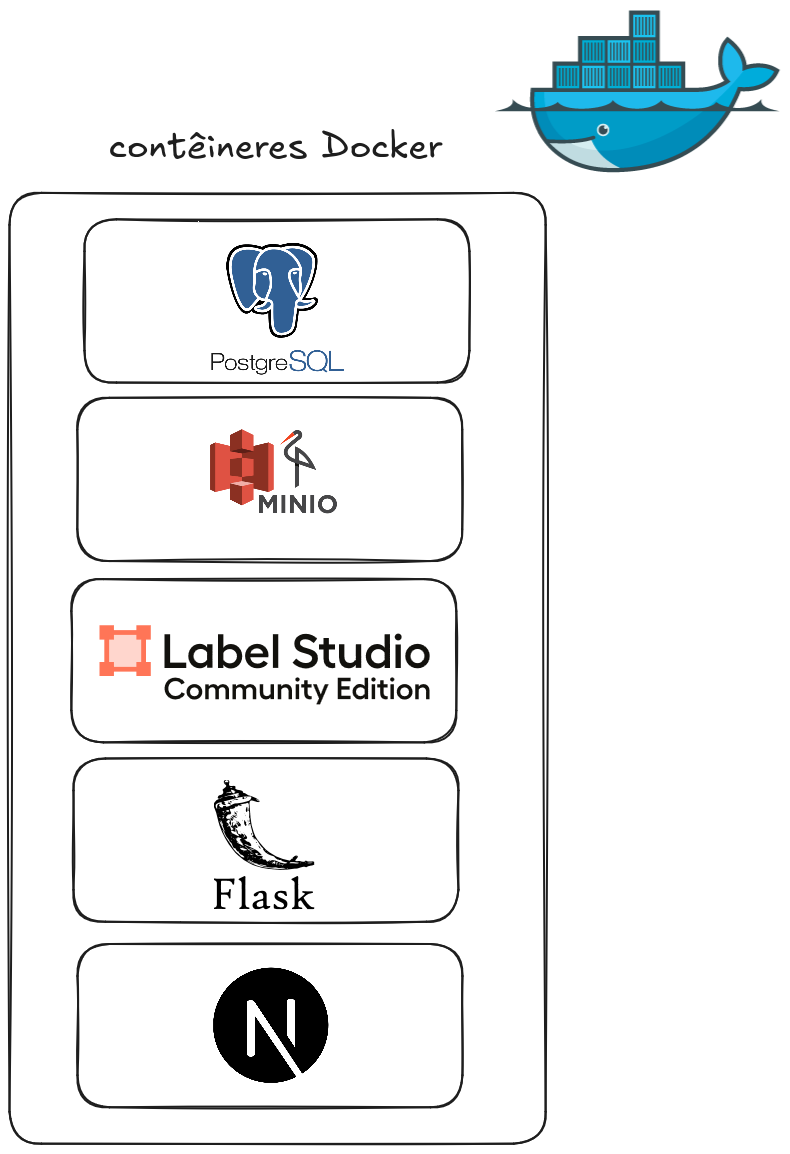
\includegraphics[height=0.5\textheight]{images/containers.png}
    \caption{\label{fig:containers} Modelo simples para os contêineres da nossa aplicação. A imagem apresenta as logos das tecnologias usadas: Docker, Next.js, Label Studio, MinIO, PostgreSQL e Flask. Fonte: acervo dos autores.}
\end{figure}

\section{\emph{Back-end}}
O \emph{back-end} do projeto foi implementado para contemplar os requisitos do capítulo \ref{sec:back-end-intro}. A maior parte do código foi feito utilizando \emph{Flask}\footnote{\url{https://flask.palletsprojects.com/en/stable/}}, um \emph{micro-framework Python} para aplicações \textit{web}.

Com essa ferramenta, implementamos os seguintes \emph{endpoints} principais (\emph{URL}s que representam funcionalidades no contexto da aplicação):
\begin{enumerate}
    \item \texttt{/process\_image}:
    \begin{enumerate}
        \item Recebe a imagem da folha do tomateiro enviada por um usuário regular;
        \item Obtém as respostas do modelo de detecção de objetos em relação às doenças presentes na imagem de folha do tomateiro:
        Isso é feito ao invocar o método de detecção de objetos do modelo de visão computacional (objeto em \emph{Python}) que é instanciado no início da aplicação
        \begin{lstlisting}
    # Run detection using YOLOv8
    detections = detection_model.predict(image, imgsz=640, conf=detection_threshold, device=device, verbose=False)
        \end{lstlisting}
        \item Salva a imagem enviada pelo usuário em um banco de dados de imagens:
        O banco de dados utilizado para a armazenagem de imagens é o \emph{S3 MinIO} \footnote{\url{https://min.io/}}, uma alternativa local ao sistema de armazenamento em nuvem \emph{S3} da AWS. Além de salvar as imagens enviadas pelos usuários, o \emph{MinIO} armazena todas as imagens do conjunto de dados em um diretório especial, no qual as imagens revisadas passarão a ser localizadas caso seja de interesse de um usuário administrador atualizar o conjunto de dados.
        \item Obtém a resposta de um modelo de linguagem que será entregue para o usuário:
        Utilizamos a \emph{API} da \emph{OpenAI}\footnote{\url{https://platform.openai.com/docs/overview}} para obter a resposta do modelo de linguagem;
        \item Envia a resposta à requisição;
    \end{enumerate}
    \item \texttt{/register\_admin}:
    Além do programa em \emph{Flask}, uma parte importante do \emph{back-end} da aplicação \emph{TomatoHealth} é um programa de linha de comando que oferece uma maneria simplificada dos administradores do sistema interagirem com ele. Com isso, é possível criar uma conta de administrador (que será registrada no banco de dados \emph{PostgreSQL}\footnote{\url{https://www.postgresql.org/}}. Com essa conta, temos acesso a todas as funcionalidades oferecidas pelo sistema, que serão explicadas a seguir.
    \item \texttt{/admin\_login}
    Depois de registrado um administrador, precisamos fazer \emph{login} na plataforma para receber um \emph{token} de autenticação \emph{JWT}. Isso é necessário pois as operações sensíveis, são protegidas.
    \item \texttt{/invite\_reviewer}
    Depois que um administrador está autenticado, ele pode convidar um usuário especialista para a plataforma. Isso é feito ao informar o \emph{e-mail} do especialista na requisição feita para \texttt{/invite\_reviewer}. Com isso, a ferramenta \emph{SendGrid} se encarrega de enviar um \emph{e-mail} convidando o usuário especialista a fazer parte da plataforma. 
    \item \texttt{/register\_reviewer/<token>}
    No \emph{e-mail} recebido pelo usuário especialista, há um link que leva para a página de registro. Essa página é renderizada pela aplicação \emph{Flask} ao acessarmos \texttt{/register\_reviewer/<token>} pelo navegador \emph{web}.
    \item \texttt{/login}
    Depois que o usuário especialista criou uma conta na plataforma, ele já pode efetuar o \emph{login}. Esse \emph{endpoint} também é renderizado pela aplicação e após um \emph{login} bem sucedido, o usuário especialista deve ser redirecionado para o endpoint \texttt{/labelling\_tool}.
    \item \texttt{/labelling\_tool}
    Nesse \emph{endpoint}, o usuário especialista será redirecionado para a plataforma de anotação das imagens enviadas pelos usuários. Então, é efetuada uma busca no banco de dados por imagens que ainda não foram revisadas. Ao encontrar uma imagem, uma tarefa no \emph{label-studio} é criada (revisão dessa imagem) e então o usuário especialista é redirecionado para essa tarefa, nesse momento, ele pode efetuar as revisões e, ao clicar no botão de finalizar a revisão, a imagem será marcada como revisada.
    \item \texttt{/update\_dataset}
    Em um momento que há diversas imagens marcadas como revisadas, um usuário administrador pode utilizar o \emph{endpoint} \texttt{/update\_dataset} para mover todas as imagens com o \emph{status} de revisadas para o diretório do \emph{MinIO} que contém o conjunto de dados inteiro.
    \item \texttt{/update\_weights}
    O processo de retreinamento do modelo (com a versão atualizada do conjunto de dados) será explicado a seguir. De qualquer maneira, um arquivo de pesos da rede neural é o resultado do treinamento e, para atualizar o modelo que está rodando na aplicação, basta enviar esse arquivo em uma requisição feita para o endpoint \texttt{/update\_weights}.
\end{enumerate}


\subsection{\emph{Machine Learning} no \emph{back-end} da aplicação}
\paragraph{Treinamento inicial:} antes de podermos iniciar a operação do sistema, seja em ambiente de desenvolvimento ou produção, um modelo de visão computacional é treinado para detectar as doenças dado uma imagem.

Após esse treinamento, obtemos um arquivo com a estrutura e os valores dos pesos do modelo treinado. Então, no programa \emph{Flask} do servidor, esse arquivo é usado para instanciar um objeto de rede neural (o modelo treinado). Assim, quando uma imagem é enviada via requisição para o endpoint \texttt{/process\_image}, obtemos os resultados das doenças detectadas pelo modelo nessa imagem ao invocar o método de inferência de seu objeto e usar a imagem recebida como argumento:
\begin{center}
\lstinline|detections = detection\_model.predict(image)|
\end{center}

\paragraph{Retreinamento:} para fazer o retreinamento do modelo de visão computacional, utilizamos o programa de linha de comando do administrador. Além disso, precisamos que o repositório do projeto esteja clonado na máquina responsável por esse processo (não só na máquina que roda a aplicação). Isso ocorre pois no repositório há um \emph{script Python} que faz o download do novo conjunto de dados do \emph{MinIO} e utiliza esses novos dados para treinar um novo modelo \emph{YOLO}. Ao final desse processo, o arquivo de pesos resultante é enviado automaticamente para o \emph{endpoint} \texttt{/update\_weights}. 

Uma funcionalidade interessante do projeto \emph{TomatoHealth} é a possibilidade de fazer o retreinamento do modelo de maneira remota (como por exemplo por meio de \emph{SSH}, isto é, acesso remoto). Para isso, um desafio importante que precisou ser superado é o fato de que precisaríamos de uma maneira de disponibilizar os dados do \emph{MinIO} e o \emph{endpoint} \texttt{/update\_weights} de alguma maneira que fosse acessível remotamente (do computador em que o retreinamento ocorre). Para isso, utilizamos a tecnologia de túnel de portas \emph{HTTP} da ferramenta \emph{Ngrok}\footnote{\url{https://ngrok.com/docs}}.


\paragraph{Uso do modelo de linguagem (\emph{LLM}):} depois de obtermos a classificação da condição das folhas identificadas na imagem, precisamos pensar em como entregar os resultados de uma maneira interessante para o usuário final.

Desse modo, implementamos uma integração dos resultados do modelo de detecção com a \emph{API} de modelos de linguagem da \emph{OpenAI}. Isso foi feito por meio da criação de um \emph{prompt} ao qual os resultados da tarefa de detecção de doenças é incorporado. Assim, o texto gerado pelo modelo de linguagem, que conterá informações sobre as doenças detectadas e dicas sobre como tratar a planta afetada é o retorno do \emph{endpoint} \texttt{/process\_image}. A estrutura do \emph{prompt} usado pode ser consultada a seguir. Note que há condições que mudam a estrutura do \emph{prompt}.

\begin{lstlisting}[literate={á}{{\'a}}1 {é}{{\'e}}1 {í}{{\'i}}1 {ó}{{\'o}}1 {ú}{{\'u}}1 {ç}{{\c{c}}}1 {ã}{{\~a}}1 {õ}{{\~o}}1]
Se nenhuma folha de tomate foi detectada:
"Não detectamos folhas de tomate na imagem."

Se apenas folhas saudáveis foram detectadas:
"De acordo com nosso algoritmo, seu tomateiro está saudável."

Caso contrário:
"A imagem de tamanho <image_width>x<image_height> pixels contém as seguintes doenças detectadas:

1. Doença: <class_name_1>
   Confiança: <score_1>
   Localização: De (<x1_1>, <y1_1>) até (<x2_1>, <y2_1>)

2. Doença: <class_name_2>
   Confiança: <score_2>
   Localização: De (<x1_2>, <y1_2>) até (<x2_2>, <y2_2>)

...

Por favor, providencie conselhos sobre como controlar e tratar as doenças detectadas e sugestões para melhorar o crescimento e a saúde da planta de tomate no geral."

Se ocorrer um erro na consulta ao modelo:
"Erro ao consultar o LLM: <mensagem_de_erro>"

\end{lstlisting}

\section{\emph{Front-end}}

\subsection{Cliente comum}

Para a interface de usuário geral, desenvolvemos duas páginas com a \textit{framework} \emph{React Next.js}, e utilizamos componentes da biblioteca \emph{React MUI}. As duas páginas são:

\begin{enumerate}
    \item página inicial
    \item página de diagnóstico do tomateiro
\end{enumerate}

Na primeira página, dividimos o site nas seguintes seções, como vistas na figura \ref{fig:homepage}, para o usuário conhecer o propósito da ferramenta e como a utilizar:

\begin{figure}[p]
    \centering
    \begin{subfigure}{0.45\textwidth}
        \centering
        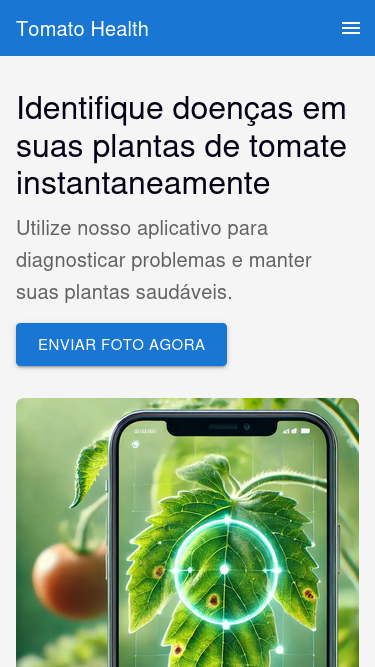
\includegraphics[width=\linewidth, height=0.4\textheight, keepaspectratio]{images/homepage1.png}
    \end{subfigure}
    \begin{subfigure}{0.45\textwidth}
        \centering
        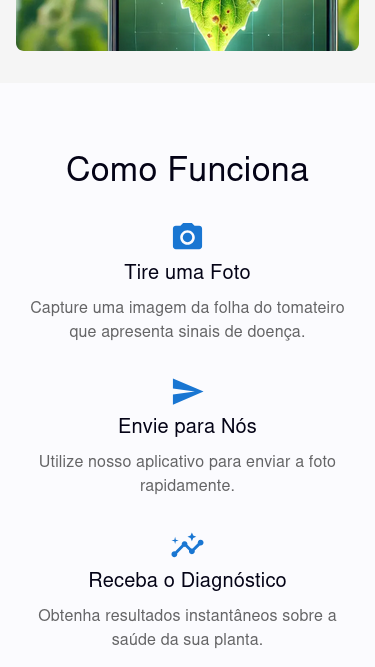
\includegraphics[width=\linewidth, height=0.4\textheight, keepaspectratio]{images/homepage2.png}
    \end{subfigure}
    
    \vspace{0.5cm}
    
    \begin{subfigure}{0.45\textwidth}
        \centering
        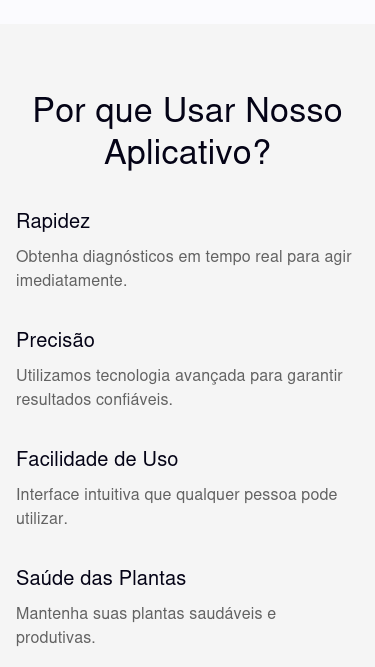
\includegraphics[width=\linewidth, height=0.4\textheight, keepaspectratio]{images/homepage3.png}
    \end{subfigure}
    \begin{subfigure}{0.45\textwidth}
        \centering
        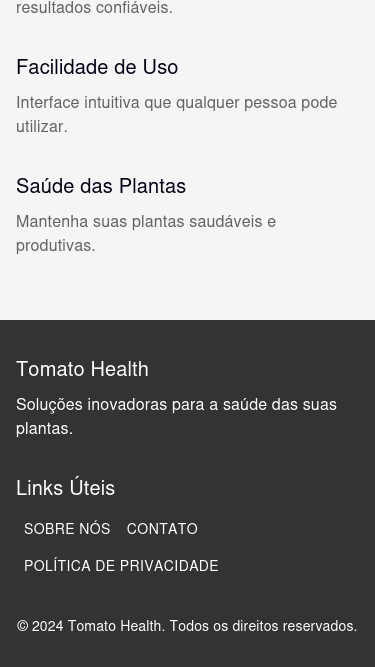
\includegraphics[width=\linewidth, height=0.4\textheight, keepaspectratio]{images/homepage4.png}
    \end{subfigure}
    
    \caption{Página inicial do TomatoHealth. Fonte da imagem utilizada: OpenAI, (2024), imagem gerada pelo modelo ChatGPT.}
    \label{fig:homepage}

\end{figure}

\begin{itemize}
    \item barra superior (\textit{app bar})
    \item destaque principal (\textit{hero section})
    \item \textit{call to action} (leva o usuário a diagnosticar sua planta)
    \item como funciona o \emph{TomatoHealth}
    \item por que usar nosso aplicativo
    \item rodapé
\end{itemize}

Na página de diagnóstico, como visto na figura \ref{fig:diagnostic}: o usuário escolhe tirar uma foto, ou então fazer \textit{upload} de sua galeria, para enviar ao servidor. O nosso \textit{front-end} então exibe a mensagem do servidor: o output de uma \emph{LLM}.

\begin{figure}[htp]
    \centering
    % Row 1
    \begin{subfigure}{0.3\textwidth}
        \centering
        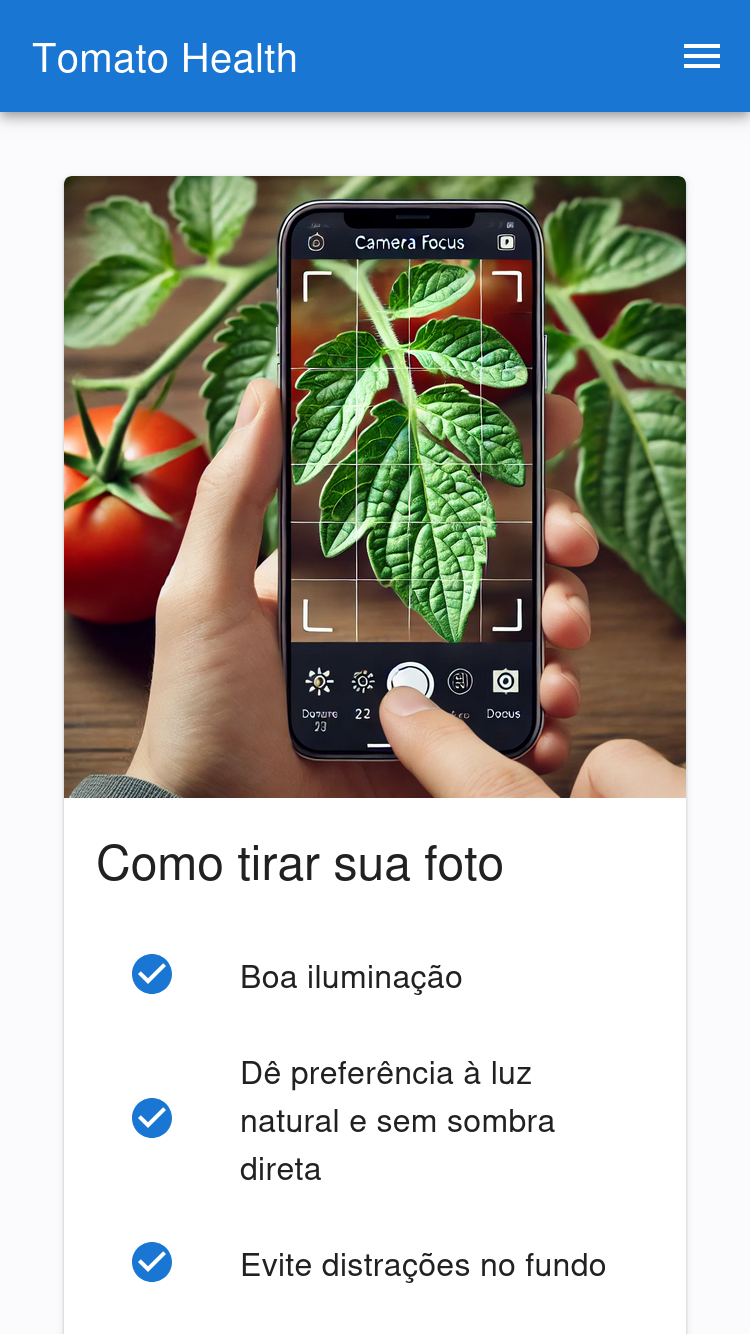
\includegraphics[width=\linewidth, height=0.4\textheight, keepaspectratio]{images/diagnostic1.png}
    \end{subfigure}
    \begin{subfigure}{0.3\textwidth}
        \centering
        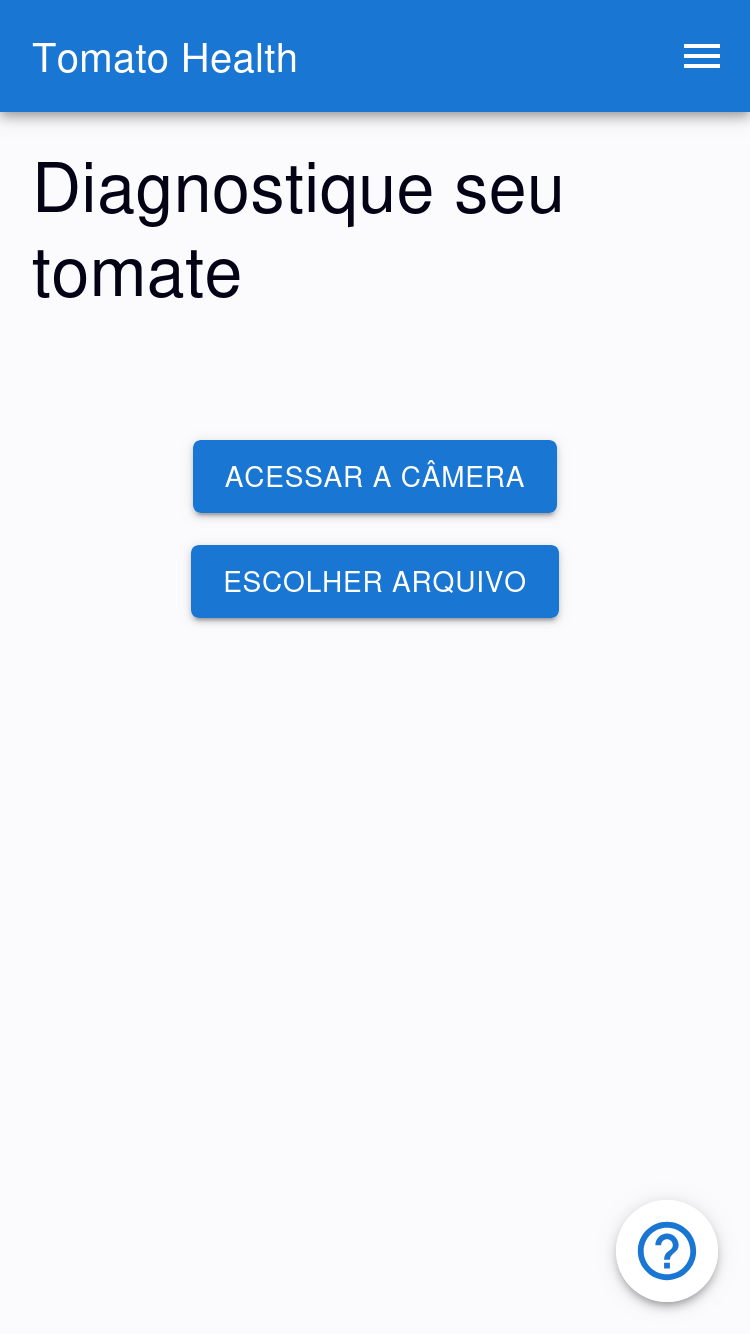
\includegraphics[width=\linewidth, height=0.4\textheight, keepaspectratio]{images/diagnostic3.png}
    \end{subfigure}
    \begin{subfigure}{0.3\textwidth}
        \centering
        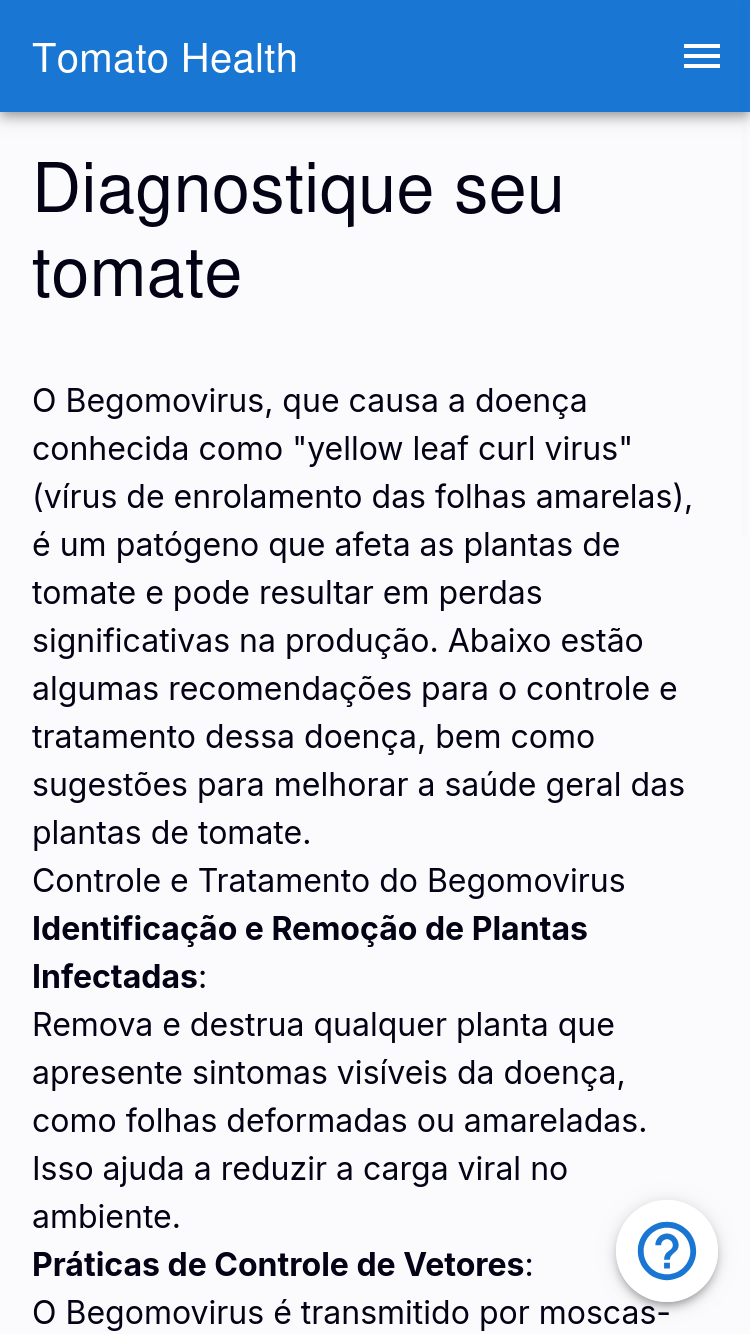
\includegraphics[width=\linewidth, height=0.4\textheight, keepaspectratio]{images/diagnostic5.png}
    \end{subfigure}
    
    % Add spacing between rows
    \vspace{0.5cm}
    
    % Row 2
    \begin{subfigure}{0.3\textwidth}
        \centering
        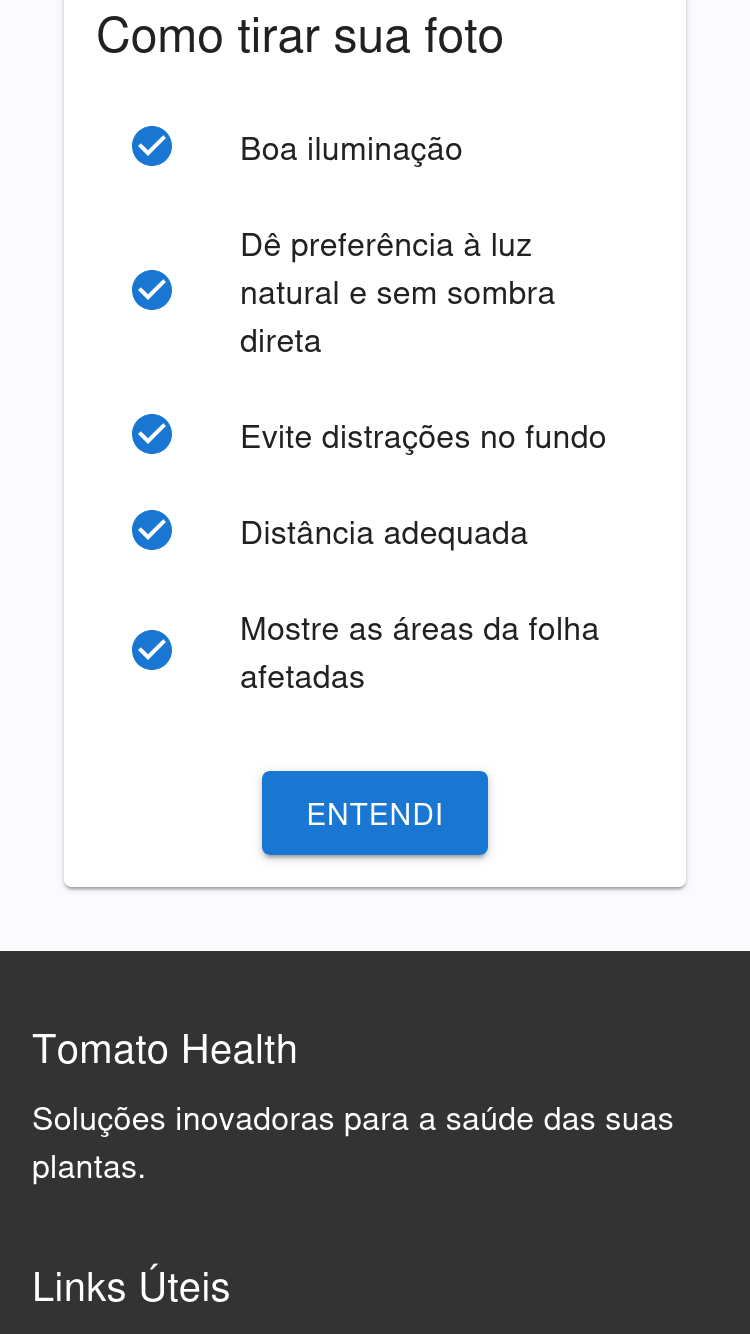
\includegraphics[width=\linewidth, height=0.4\textheight, keepaspectratio]{images/diagnostic2.png}
    \end{subfigure}
    \begin{subfigure}{0.3\textwidth}
        \centering
        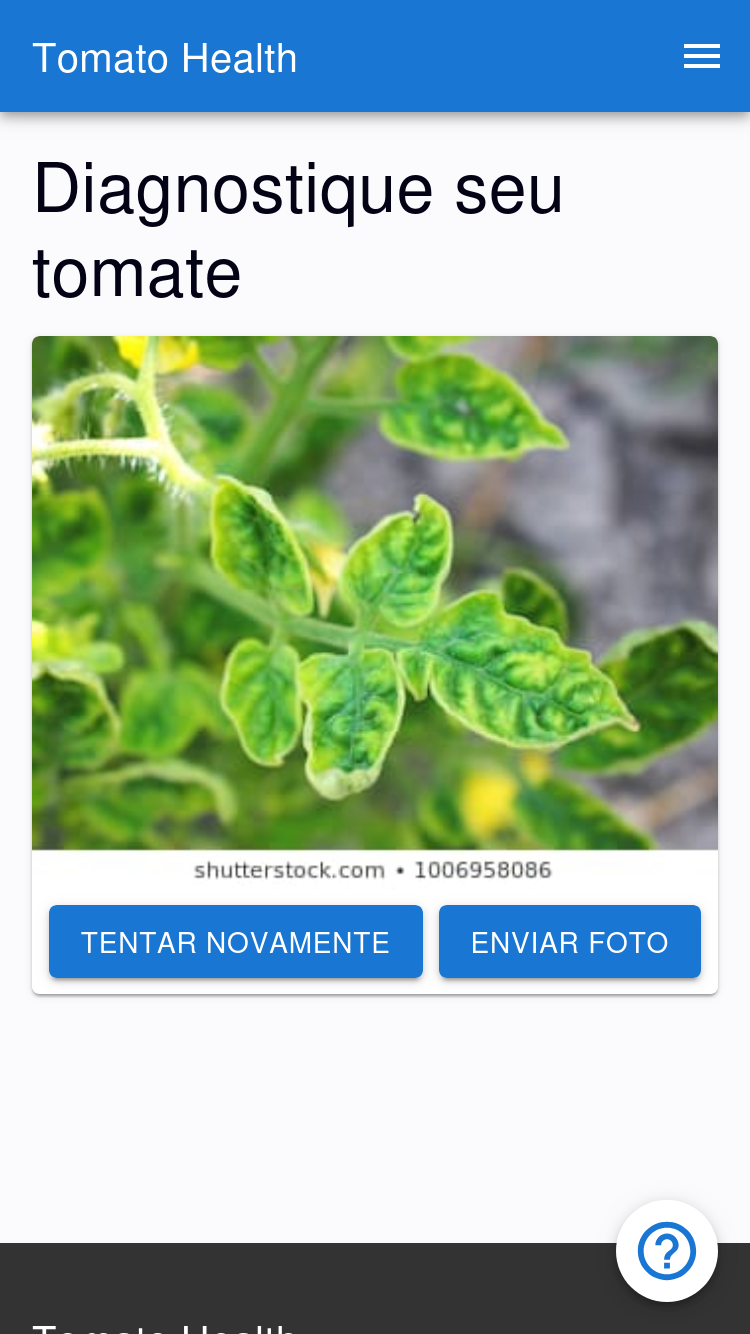
\includegraphics[width=\linewidth, height=0.4\textheight, keepaspectratio]{images/diagnostic4.png}
    \end{subfigure}
    \begin{subfigure}{0.3\textwidth}
        \centering
        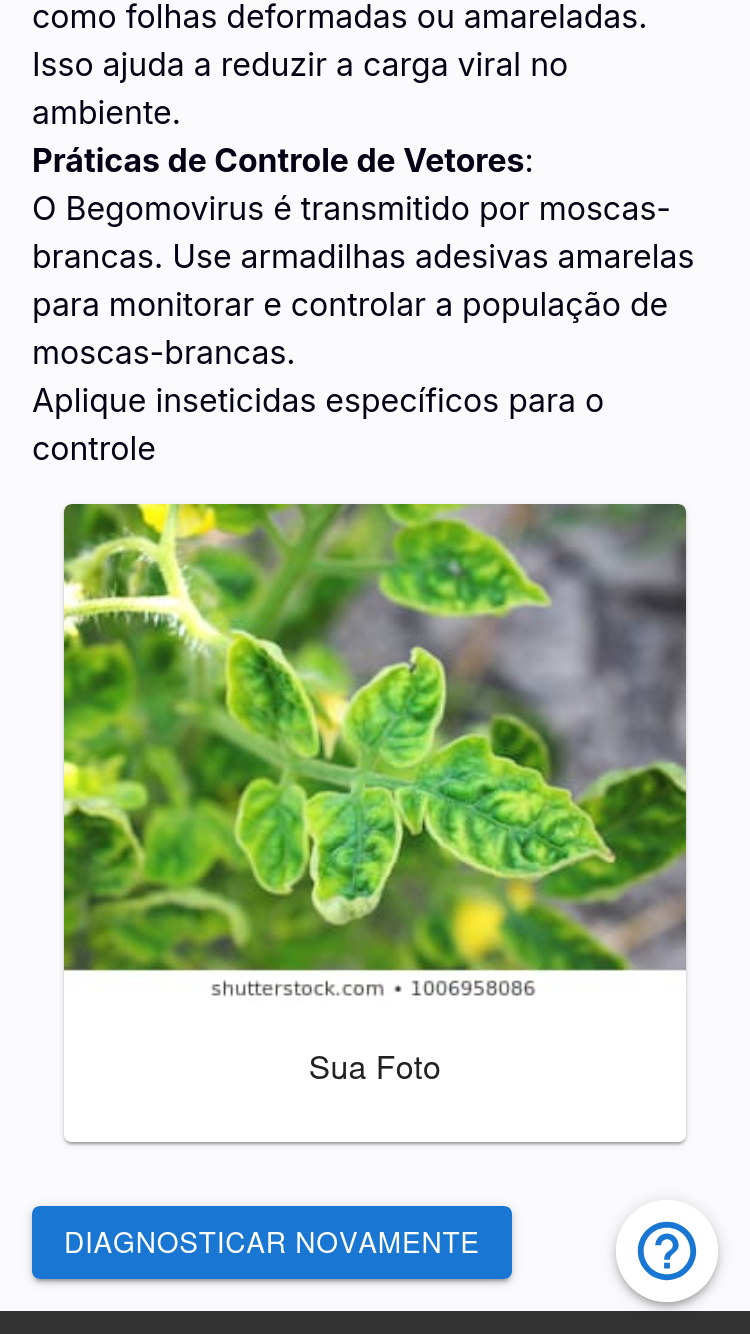
\includegraphics[width=\linewidth, height=0.4\textheight, keepaspectratio]{images/diagnostic6.png}
    \end{subfigure}
    
    \caption{Página de diagnóstico do TomatoHealth. Fonte da imagem utilizada: OpenAI, (2024), imagem gerada pelo modelo ChatGPT.}        
    \label{fig:diagnostic}
\end{figure}


\subsection{Cliente especialista e ferramenta de anotação \emph{Label Studio}}

Na interface do usuário especialista, utilizamos o \textit{software open-source} de rotulagem \emph{Label Studio}. Segundo sua página no \emph{Github}, "O Label Studio é uma ferramenta de rotulagem de dados de código aberto. Ela permite rotular tipos de dados como áudio, texto, imagens, vídeos e séries temporais com uma interface de usuário simples e direta e exportar para vários formatos de modelos. Ele pode ser usado para preparar dados brutos ou melhorar os dados de treinamento existentes para obter modelos de ML mais precisos".

Para não exibir detalhes desnecessários do sistema, modificamos seu código \textit{front-end} em \emph{React}, de forma a excluir alguns componentes da página de anotação, como barras nas laterais e no topo da página, com a finalidade do usuário não visitar endereços não utilizadas pelo \emph{TomatoHealth}.

Conforme a figura \ref{fig:rotulagem_labelstudio}, o usuário especialista vê, por vez, uma única imagem que ele poderá demarcar classes de doenças com \textit{bounding boxes}. Após ele efetuar a rotulagem, o banco de dados é atualizado com as novas informações e o usuário é redirecionado para a próxima imagem.

\begin{figure}[htbp]
    \centering
    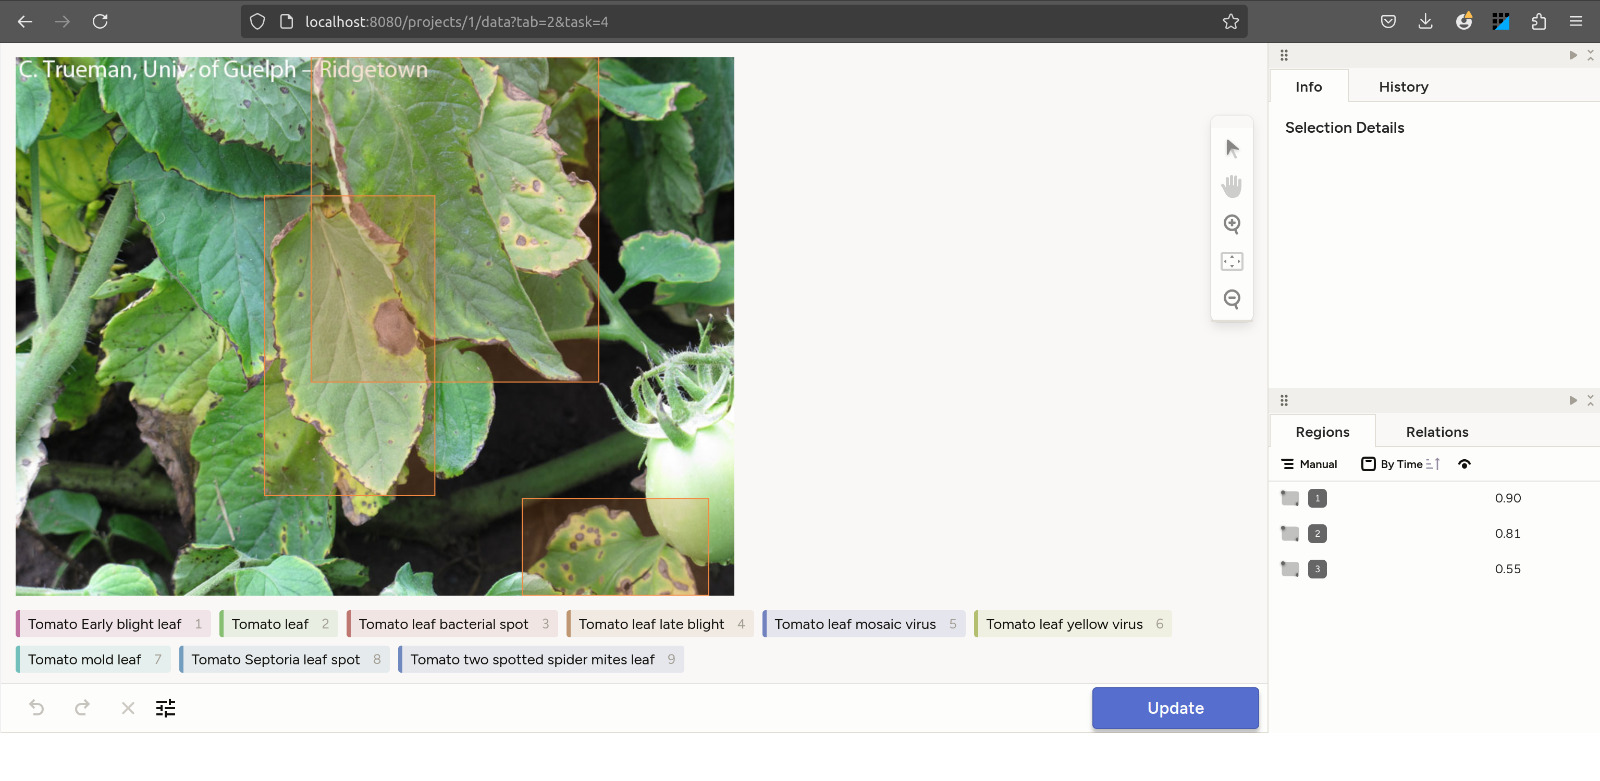
\includegraphics[width=1\linewidth]{images/rotulagem_labelstudio.jpg}
    \caption{\label{fig:rotulagem_labelstudio} Página de rotulagem do usuário especialista utilizando uma versão modificada do Label Studio. Fonte: acervo dos autores.}
\end{figure}

\chapter{Próximos passos}
\label{sec:próximos passos}
\section{Integrando os \emph{datasets}}
\label{sec:integrando-resultados}
Como comentado anteriormente, embora o \emph{TomatoHealth} seja um projeto que tem o objetivo de construir um conjunto de dados robusto que possibilite o treinamento de modelos confiáveis e eficientes na tarefa de detecção de doenças em folhas de plantas, acreditamos que a performance inicial do modelo oferecido pela plataforma pode ser uma variável determinante para atrair um número considerável de usuários.

Com esse engajamento inicial, o objetivo do projeto se torna mais facilmente alcançável, pois esses primeiros usuários irão contribuir ativamente para o aumento da quantidade de imagens que poderão fazer parte das novas versões dos conjuntos de dados criados pelo \emph{TomatoHealth}. Portanto, consideramos como um próximo passo do desenvolvimento do projeto, uma tarefa que aumenta a quantidade de dados disponíveis na primeira versão do \emph{dataset} utilizado e, por isso, pode ser que produza um modelo inicialmente mais eficaz do que o atual.

Essa estratégia consiste em integrar o \emph{dataset PlantVillage} com o conjunto de dados obtido a partir do processamento do \emph{PlantDoc}. Apesar dos problemas previamente discutidos em relação ao \emph{PlantVillage}, acreditamos que essa integração pode beneficiar a eficiência do modelo inicial do \emph{TomatoHealth}. Essa abordagem é particularmente interessante porque o número de exemplos atualmente presentes no conjunto de dados do projeto é muito pequeno, enquanto o \emph{PlantVillage} oferece uma quantidade consideravelmente maior de exemplos, o que pode contribuir para um treinamento mais robusto.

Na figura \ref{fig:distribuicao_plantvillage}, observamos a distribuição de imagens por classes de doenças em folhas de tomate presentes no conjunto de dados \emph{PlantVillage}. Note que as classes do \emph{PlantDoc} representam um subconjunto das classes do \emph{PlantVillage}. A classe \texttt{Tomato\_\_\_Target\_Spot}, embora não esteja presente no \emph{PlantDoc}, poderia ser incorporada como uma possível adição futura.

\begin{figure}[H]
    \centering
    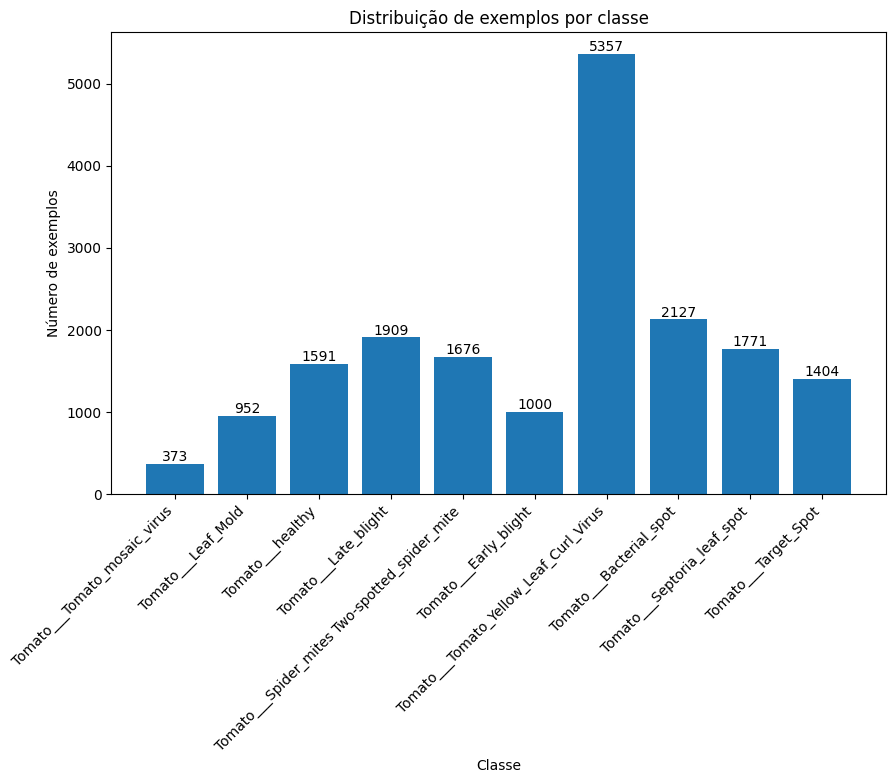
\includegraphics[width=0.9\linewidth]{images/plant_village_distribution.png}
    \caption{\label{fig:distribuicao_plantvillage} Distribuição de exemplos por classes de tomate no \emph{PlantVillage}. Fonte: acervo dos autores.}
\end{figure}

Como o \emph{PlantVillage} possui uma única folha por imagem e é destinado à tarefa de classificação, a ideia para fazer essa integração é utilizar a área inteira das imagens do \emph{PlantVillage} como \emph{bounding box}.

\section{Busca de imagens por similaridade}
Como comentado anteriormente, é importante que um conjunto de dados robusto não tenha duplicatas ou ``quase-duplicatas'' em seus dados. No sistema atual, não há uma maneira de assegurar que somente imagens distintas farão parte do conjunto de dados resultante. Nesse sentido, para que os conjuntos de dados produzidos pelo \emph{TomatoHealth} não tenham dados repetidos, pensamos em um próximo passo que apresente as imagens mais semelhantes à que está sendo revisada. Assim, caso o usuário especialista interprete que ela é semelhante demais com imagens já presentes no conjunto de dados atual, será possível cancelar sua adição ao conjunto de dados atualizado.

Para fazer isso, pensamos no seguinte passo a passo:
\begin{enumerate}
    {\bf  \item Produzir representações em alto nível de cada imagem que faz parte do conjunto de dados:} essas representações, também conhecidas como \emph{embeddings}, não são nada mais que o resultado da extração de características de cada imagem. É mais simples e eficiente armazenar e comparar uma imagem com as demais se ela for representada como um vetor de 512 dimensões, por exemplo, ao invés de uma matriz de \emph{pixels} de $256 \times 256 \times 3$ dimensões.
    {\bf \item Armazenar esses \emph{embeddings} em um banco de dados de vetores:} podemos utilizar modelos de redes convolucionais pré-treinadas no \emph{dataset ImageNet}, boas em extração de características, para produzir os \emph{embeddings} de todas as imagens o conjunto de dados e então armazenar essas extrações em um banco de dados de vetores. Isso é importante pois, assim, só precisaremos obter essas representações uma única vez. Seguindo essa lógica, depois da revisão de toda imagem por um usuário especialista, devemos produzir sua representação vetorial e armazená-la no banco de dados vetorial.
    {\bf \item Fazer busca por similaridade no banco de dados vetorial:} no momento em que um usuário especialista for fazer a revisão de uma nova imagem, devemos fazer a busca por similaridade com as imagens presentes no banco de dados vetorial e, por conseguinte, no conjunto de dados. Isso é uma tarefa recorrente e há diversas ferramentas que disponibilizam esse serviço. Podemos comentar sobre a \emph{Pinecone}\footnote{\url{https://www.pinecone.io/learn/what-is-similarity-search/\#What-Are-Vector-Representations}}, que inclusive disponibiliza uma busca pelos $K$ vetores mais semelhantes ao examinado.
     {\bf \item Exibir as imagens mais semelhantes:} basta exibir as imagens mais semelhantes ao usuário especialista.
\end{enumerate}

\section{Mudança de \emph{LLM}}

Atualmente, como descrito no artigo, utilizamos uma chamada de \textit{API} a um modelo de linguagem (\texttt{gpt-4o-mini}) disponibilizado pela \textit{OpenAI} para gerar a resposta de diagnóstico ao usuário. No entanto, tal serviço é pago e adiciona dependências à serviços de terceiros ao projeto \emph{TomatoHealth}. Dessa forma, é interessante trabalhar para que essa funcionalidade seja incorporada de maneira mais natural ao projeto, sem implicar em custos monetários e que seja independente de terceiros. Isso pode ser feito com a adição um programa que rode um modelo de linguagem (\emph{LLM}) como um \emph{container} no ecossistema do \emph{Docker Compose}. Para isso, poderíamos utilizar a ferramenta \emph{HuggingFace Transformers}\footnote{\url{https://huggingface.co/docs/transformers/index}}, que torna simples o processo de inferência e treinamento de modelos de linguagem atuais.

\chapter{Conclusão}
Ao longo desse trabalho, a importância do desenvolvimento de soluções baratas e eficientes para a detecção e diagnóstico de doenças na produção agrícola ficou evidente. A análise da situação atual dos conjuntos de dados abertos e das aplicações baseadas neles revelou limitações significativas, como problemas de qualidade e uma relativa escassez de dados, que comprometem a eficácia dessas iniciativas.

Então, fica claro que o desenvolvimento dessas soluções exige a criação de conjuntos de dados abertos, livres e robustos capazes de sustentar o desenvolvimento de aplicações voltadas ao diagnóstico e à detecção de doenças em plantas por meio de imagens. Essa abordagem beneficia os agricultores e a comunidade científica em geral.

O objetivo deste trabalho de formatura foi justamente implementar uma solução promissora para essa demanda: o sistema \emph{TomatoHealth}. Um sistema que oferece uma interface intuitiva para que agricultores diagnostiquem doenças em suas plantas --- inicialmente voltada para tomateiros, mas com potencial de expansão para outras culturas. Para efetuar essa tarefa, o \emph{TomatoHealth} conta com um modelo de detecção de objetos (\emph{YOLOv8}) que inicialmente foi treinado com um subconjunto do \emph{dataset PlantDoc}.

O diferencial do \emph{TomatoHealth} está na possibilidade de melhoria contínua do conjunto de dados. As imagens enviadas pelos usuários passam pela revisão de especialistas e, então, são incorporadas ao conjunto de dados original. Ainda, podemos utilizar o novo conjunto de dados para retreinar o modelo de detecção de objetos e melhorar o desempenho da ferramenta de diagnóstico do \emph{TomatoHealth}. Esse processo melhora o desempenho do diagnóstico e contribui para a construção de um \emph{dataset} mais representativo das condições reais, já que utiliza fotos capturadas por dispositivos móveis diretamente em campo.

Por fim, este trabalho busca transformar a forma como os conjuntos de dados são produzidos, promovendo o desenvolvimento de soluções mais acessíveis e abertas. Essa abordagem, além de democratizar o acesso à tecnologia, visa expandir o alcance do conhecimento e impulsionar o progresso científico de maneira inclusiva.



%%%%%%%%%%%%%%% SEÇÕES FINAIS (BIBLIOGRAFIA E ÍNDICE REMISSIVO) %%%%%%%%%%%%%%%%

% O comando backmatter desabilita a numeração de capítulos.
\backmatter

\pagestyle{backmatter}

% Espaço adicional no sumário antes das referências / índice remissivo
\addtocontents{toc}{\vspace{2\baselineskip plus .5\baselineskip minus .5\baselineskip}}

% A bibliografia é obrigatória

\printbibliography[
  title=\refname\label{sec:bib}, % "Referências", recomendado pela ABNT
  %title=\bibname\label{sec:bib}, % "Bibliografia"
  heading=bibintoc, % Inclui a bibliografia no sumário
]

\printindex % imprime o índice remissivo no documento (opcional)

\end{document}
